%% (Master) Thesis template
% Template version used: v1.4
%
% Largely adapted from Adrian Nievergelt's template for the ADPS
% (lecture notes) project.


%% We use the memoir class because it offers a many easy to use features.
\documentclass[11pt,a4paper]{memoir}

%% CUSTOM Marc: Decrease Margins
\setlrmarginsandblock{3cm}{3cm}{*}
\setulmarginsandblock{3cm}{*}{1}
\checkandfixthelayout 

%% Packages
%% ========

%% LaTeX Font encoding -- DO NOT CHANGE
\usepackage[OT1]{fontenc}

%% Babel provides support for languages.  'english' uses British
%% English hyphenation and text snippets like "Figure" and
%% "Theorem". Use the option 'ngerman' if your document is in German.
%% Use 'american' for American English.  Note that if you change this,
%% the next LaTeX run may show spurious errors.  Simply run it again.
%% If they persist, remove the .aux file and try again.
\usepackage[english]{babel}

%% Input encoding 'utf8'. In some cases you might need 'utf8x' for
%% extra symbols. Not all editors, especially on Windows, are UTF-8
%% capable, so you may want to use 'latin1' instead.
\usepackage[utf8]{inputenc}

%% This changes default fonts for both text and math mode to use Herman Zapfs
%% excellent Palatino font.  Do not change this.
\usepackage[sc]{mathpazo}

%% The AMS-LaTeX extensions for mathematical typesetting.  Do not
%% remove.
\usepackage{amsmath,amssymb,amsfonts,mathrsfs}

%% NTheorem is a reimplementation of the AMS Theorem package. This
%% will allow us to typeset theorems like examples, proofs and
%% similar.  Do not remove.
%% NOTE: Must be loaded AFTER amsmath, or the \qed placement will
%% break
\usepackage[amsmath,thmmarks]{ntheorem}

%% LaTeX' own graphics handling
\usepackage{graphicx}


%% This allows you to add .pdf files. It is used to add the
%% declaration of originality.
\usepackage{pdfpages}

\usepackage{realboxes}
\usepackage{listings}
\lstdefinelanguage{none}{
  identifierstyle=
}
\definecolor{backcolor}{rgb}{0.95,0.95,0.92}
\lstdefinestyle{mystyle}{
    backgroundcolor=\color{backcolor}
}
\newcommand{\inline}[1]{\Colorbox{backcolor}{\lstinline[language=C]{#1}}}



%% Our layout configuration.  DO NOT CHANGE.
%% Memoir layout setup

%% NOTE: You are strongly advised not to change any of them unless you
%% know what you are doing.  These settings strongly interact in the
%% final look of the document.

% Dependencies
\usepackage{ETHlogo}

% Turn extra space before chapter headings off.
\setlength{\beforechapskip}{0pt}

\nonzeroparskip
\parindent=0pt
\defaultlists

% Chapter style redefinition
\makeatletter

\if@twoside
  \pagestyle{Ruled}
  \copypagestyle{chapter}{Ruled}
\else
  \pagestyle{ruled}
  \copypagestyle{chapter}{ruled}
\fi
\makeoddhead{chapter}{}{}{}
\makeevenhead{chapter}{}{}{}
\makeheadrule{chapter}{\textwidth}{0pt}
\copypagestyle{abstract}{empty}

\makechapterstyle{bianchimod}{%
  \chapterstyle{default}
  \renewcommand*{\chapnamefont}{\normalfont\Large\sffamily}
  \renewcommand*{\chapnumfont}{\normalfont\Large\sffamily}
  \renewcommand*{\printchaptername}{%
    \chapnamefont\centering\@chapapp}
  \renewcommand*{\printchapternum}{\chapnumfont {\thechapter}}
  \renewcommand*{\chaptitlefont}{\normalfont\huge\sffamily}
  \renewcommand*{\printchaptertitle}[1]{%
    \hrule\vskip\onelineskip \centering \chaptitlefont\textbf{\vphantom{gyM}##1}\par}
  \renewcommand*{\afterchaptertitle}{\vskip\onelineskip \hrule\vskip
    \afterchapskip}
  \renewcommand*{\printchapternonum}{%
    \vphantom{\chapnumfont {9}}\afterchapternum}}

% Use the newly defined style
\chapterstyle{bianchimod}

\setsecheadstyle{\Large\bfseries\sffamily}
\setsubsecheadstyle{\large\bfseries\sffamily}
\setsubsubsecheadstyle{\bfseries\sffamily}
\setparaheadstyle{\normalsize\bfseries\sffamily}
\setsubparaheadstyle{\normalsize\itshape\sffamily}
\setsubparaindent{0pt}

% Set captions to a more separated style for clearness
\captionnamefont{\sffamily\bfseries\footnotesize}
\captiontitlefont{\sffamily\footnotesize}
\setlength{\intextsep}{16pt}
\setlength{\belowcaptionskip}{1pt}

% Set section and TOC numbering depth to subsection
\setsecnumdepth{subsection}
\settocdepth{subsection}

%% Titlepage adjustments
\pretitle{\vspace{0pt plus 0.7fill}\begin{center}\HUGE\sffamily\bfseries}
\posttitle{\end{center}\par}
\preauthor{\par\begin{center}\let\and\\\Large\sffamily}
\postauthor{\end{center}}
\predate{\par\begin{center}\Large\sffamily}
\postdate{\end{center}}

\def\@advisors{}
\newcommand{\advisors}[1]{\def\@advisors{#1}}
\def\@department{}
\newcommand{\department}[1]{\def\@department{#1}}
\def\@thesistype{}
\newcommand{\thesistype}[1]{\def\@thesistype{#1}}

\renewcommand{\maketitlehooka}{\noindent\ETHlogo[2in]}

\renewcommand{\maketitlehookb}{\vspace{1in}%
  \par\begin{center}\Large\sffamily\@thesistype\end{center}}

\renewcommand{\maketitlehookd}{%
  \vfill\par
  \begin{flushright}
    \sffamily
    \@advisors\par
    \@department, ETH Zurich
  \end{flushright}
}

\checkandfixthelayout

\setlength{\droptitle}{-48pt}

\makeatother

% This defines how theorems should look. Best leave as is.
\theoremstyle{plain}
\setlength\theorempostskipamount{0pt}

%%% Local Variables:
%%% mode: latex
%%% TeX-master: "thesis"
%%% End:


%% Theorem environments.  You will have to adapt this for a German
%% thesis.
%% Theorem-like environments

%% This can be changed according to language. You can comment out the ones you
%% don't need.

\numberwithin{equation}{chapter}

%% German theorems
%\newtheorem{satz}{Satz}[chapter]
%\newtheorem{beispiel}[satz]{Beispiel}
%\newtheorem{bemerkung}[satz]{Bemerkung}
%\newtheorem{korrolar}[satz]{Korrolar}
%\newtheorem{definition}[satz]{Definition}
%\newtheorem{lemma}[satz]{Lemma}
%\newtheorem{proposition}[satz]{Proposition}

%% English variants
\newtheorem{theorem}{Theorem}[chapter]
\newtheorem{example}[theorem]{Example}
\newtheorem{remark}[theorem]{Remark}
\newtheorem{corollary}[theorem]{Corollary}
\newtheorem{definition}[theorem]{Definition}
\newtheorem{lemma}[theorem]{Lemma}
\newtheorem{proposition}[theorem]{Proposition}

\newtheorem{conjecture}[theorem]{Conjecture}

%% Proof environment with a small square as a "qed" symbol
\theoremstyle{nonumberplain}
\theorembodyfont{\normalfont}
\theoremsymbol{\ensuremath{\square}}
\newtheorem{proof}{Proof}
%\newtheorem{beweis}{Beweis}



%% Make document internal hyperlinks wherever possible. (TOC, references)
%% This MUST be loaded after varioref, which is loaded in 'extrapackages'
%% above.  We just load it last to be safe.
\usepackage[linkcolor=black,colorlinks=true,citecolor=black,filecolor=black]{hyperref}

% ######## CUSTOM package load before cleverref ########
\RequirePackage{silence}
\WarningFilter{latexfont}{Font shape `}
\WarningFilter{latexfont}{Size substitutions}

\usepackage{stmaryrd}
\usepackage[advantage,adversary,sets,ff,primitives,events,keys,notions]{cryptocode}
\usepackage{siunitx}

\usepackage{multirow}
\usepackage{adjustbox}
\usepackage{xspace}
% ######## END CUSTOM package load ########

%% This allows you to use "\cref{sec:your-section}" instead of writing out 
%% "Section~\ref{sec:your-section}", also works for tables, figures, etc.
%% Use \Cref at the beginning of a sentence and \cref elsewhere.
%% Must be loaded after hyperref.
\usepackage[capitalise]{cleveref}


%% Document information
%% ====================

\title{Implementing and Evaluating Quantum-Safe Fully Encrypted Protocols}
\author{Marc Himmelberger}
\thesistype{Master's Thesis}
\advisors{Advisors: Prof.~Kenneth G. Paterson, Dr.~Felix Günther (IBM Research - Zürich), Shannon Veitch}
\department{Applied Cryptography Group\\Institute of Information Security\\Department of Computer Science}
\date{June 20, 2025}

% ######## CUSTOM style code ########
\lstdefinestyle{myStyle}{
    breaklines=true,
    frame=leftline,
    numbers=left,
    backgroundcolor=\color{gray!10!white},
}
\lstset{style=myStyle}

\newcolumntype{L}[1]{>{\raggedright\arraybackslash}p{#1}}
\newcolumntype{R}[1]{>{\raggedleft\arraybackslash}p{#1}}
\newcommand{\getsr}{\xleftarrow{\smash{\raisebox{-1.75pt}{$\scriptscriptstyle\$$}}}}
\newcommand{\tor}{\xrightarrow{\smash{\raisebox{-1.75pt}{$\scriptscriptstyle\$$}}}}
\newcommand{\ul}[1]{\underline{\smash{#1}}}  % tight underline
\newcommand{\KEM}{\ensuremath{\mathsf{KEM}}}
\newcommand{\OKEM}{\ensuremath{\mathsf{OKEM}}}
\newcommand{\pkcoll}[1]{\pcnotionstyle{pkcoll}_{#1}}
\newcommand{\obfpklen}{{\mathsf{pl}_\OKEM}}
\newcommand{\obfctxtlen}{{\mathsf{cl}_\OKEM}}
\newcommand{\pklen}{{\mathsf{pl}_\KEM}}
\newcommand{\ctxtlen}{{\mathsf{cl}_\KEM}}
\newcommand{\pkobf}{\hat{\pk}}

\newcommand{\simulbin}{\mathcal{S}_\$}
\newcommand{\simulunif}{\mathcal{S}_\mathcal{C}}

\newcommand{\feo}{\textsf{\textnormal{FEO}}}

\newcommand{\obfsfour}{\textsf{obfs4}}
\newcommand{\pqobfs}{\textsf{pq-obfs}}
\newcommand{\drivel}{\textsf{drivel}}

\newcommand{\gopkgref}[2]{\href{https://pkg.go.dev/#1@#2}{#1} #2}

\pcfixcleveref

% Define aliases
\renewcommand{\pcadvantagename}{\mathsf{Adv}}
\renewcommand{\pcadvantagesuperstyle}[1]{#1}
\renewcommand{\pcadvantagesubstyle}[1]{#1}

% Set up style for algorithms
\definecolor{lngray}{gray}{0.5} % gray line numbers
\renewcommand{\pclnspace}{0.5em} % spacing of numbering
\renewcommand{\pclnrspace}{0em}
\renewcommand{\pclnstyle}[1]{\text{\scriptsize\color{lngray} \num[minimum-integer-digits=2]{#1}}} % zero-pad
\renewcommand{\pclnseparator}{} % no separator
\makeatletter % put comments at the end of lines, could not do it just with hfill & fiends so I dug into internals :P
\newcommand{\lncomment}[1]{ \@pc@modeend& \mbox{\pccomment{}\hspace{-0.75em} \ensuremath{#1}} \\  }
\newcommand{\titlecomment}[1]{ \hfill \mbox{\pccomment{}\hspace{-0.75em} \ensuremath{#1}}}
\makeatother
% Refine cryptocode styles and add more notions
\renewcommand{\pcnotionstyle}[1]{\ensuremath{\mathsf{#1}}}
\renewcommand{\kgen}{\pcalgostyle{KeyGen}}

\providecommand{\encaps}{\pcalgostyle{Encaps}}
\providecommand{\decaps}{\pcalgostyle{Decaps}}
\providecommand{\decapsoracle}{\mathcal{O}_{\decaps}}
\providecommand{\filterpk}{\pcalgostyle{FilterPk}}
\providecommand{\encodectxt}{\pcalgostyle{EncodeCtxt}}
\providecommand{\decodectxt}{\pcalgostyle{DecodeCtxt}}
\providecommand{\sprcca}{\pcnotionstyle{SPR\pcmathhyphen{}CCA}}
\providecommand{\sprcpa}{\pcnotionstyle{SPR\pcmathhyphen{}CPA}}

\providecommand{\sObfKE}{\pcnotionstyle{sObfKE}}
\providecommand{\swapprf}{\pcnotionstyle{swap\pcmathhyphen{}PRF}}
\providecommand{\indonecca}{\pcnotionstyle{IND\pcmathhyphen{}1CCA}}

\providecommand{\firstkeygensuccess}{\pcnotionstyle{1kgensucc}}
\providecommand{\firstencapssuccess}{\pcnotionstyle{1encsucc}}

\providecommand{\pkunif}{\pcnotionstyle{pk\pcmathhyphen{}unif}}
\providecommand{\ctxtunif}{\pcnotionstyle{ctxt\pcmathhyphen{}unif}}

\providecommand{\prkey}{\pcnotionstyle{PR\pcmathhyphen{}Key}}
\providecommand{\mdsd}{\pcnotionstyle{mDSD}}
\providecommand{\skdsd}{\pcnotionstyle{skDSD}}


\providecommand{\twodqcsd}{\pcnotionstyle{2\pcmathhyphen{}DQCSD}}
\providecommand{\threedqcsd}{\pcnotionstyle{3\pcmathhyphen{}DQCSD}}

\providecommand{\sObf}{\pcnotionstyle{sObf}}

% ######## Start macros.tex

\definecolor{RoyalBlue}{RGB}{65,105,225}

% ClientAction and ServerAction
% Print a command executed by the client/server
% main argument: the text, optional argument: tikz modifier
\newcommand{\ClientAction}[2][]{
	\node[right,#1] at (\ClientX, \Y) {#2};
}
\newcommand{\ServerAction}[2][]{
	\node[left,#1] at (\ServerX, \Y) {#2};
}
\newcommand{\ServerActionLeft}[2][]{
	\ServerAction[text width=\ServerLeftTextwidth,align=left,#1]{#2}
}
\newcommand{\SharedAction}[2][]{
	\node[#1] at ($1/2*(\ClientX, \Y)+1/2*(\ServerX, \Y)$) {#2};
}

% ClientToServer and ServerToClient
% Draws a message flow from client-to-server or server-to-client, with text above and below
% 1st argument (optional): line type, default ->
% 2nd argument: text above
% 3rd argument: text below
% Example: \ClientToServer{$Y$}{}
% Example: \ClientToServer[<->,double]{$Y$}{over an encrypted channel}
\newcommand{\ClientToServer}[3][->]{
	\NextLine[0.5]
	\draw[#1] (\ArrowLeft,\Y) -- node[above] {#2} node[below] {#3} (\ArrowRight,\Y) ;
	% \NextLine[0.5]
}
\newcommand{\ServerToClient}[3][->]{
	\NextLine[0.5]
	\draw[#1] (\ArrowRight,\Y) -- node[above] {#2} node[below] {#3} (\ArrowLeft,\Y) ;
	% \NextLine[0.5]
}
% Draws a horizontal line across the entire page to denote the start and end of protocol phases
% 1st argument (optional): line type, default "dotted"
% 2nd argument: text above
% 3rd argument: text below
\newcommand{\PhaseBreak}[3][dotted]{
	\NextLine[0.5]
	\draw[#1] (\ClientX,\Y) -- node[above] {#2} node[below] {#3} (\ServerX,\Y) ;
	% \NextLine[0.5]
}

% Spacing factor for NextLines
\def\NextLineSpacing{0.45}

% NextLine
% 1st argument (optional): amount of spacing to increment by, default 1.0
% Example: \NextLine
% Example: \NextLine[1.5]
\newcommand{\NextLine}[1][1.0]{
	\pgfmathparse{\Y-\NextLineSpacing*#1}
	\edef\Y{\pgfmathresult}
}


\newcommand{\highlightbox}[2][RoyalBlue!20]{\adjustbox{cframe=#1, bgcolor=#1}{\strut #2}}

\providecommand{\nodeid}{\ensuremath{\mathsf{NodeID}}}
\providecommand{\nodeidlen}{\ensuremath{\mathsf{nl}}}
\providecommand{\pstate}{\ensuremath{\mathsf{st}}}
\providecommand{\macregister}{\ensuremath{\mathcal{S}_\mathsf{MAC}}}
\providecommand{\cpaddist}{\ensuremath{\mathcal{D}_\mathsf{pad}_C}}
\providecommand{\cpaddist}{\ensuremath{\mathcal{D}_\mathsf{pad}_S}}

\newcommand{\funPRF}{\ensuremath{\pcalgostyle{F}_1}\xspace}
\newcommand{\funPRFoutlen}{\ensuremath{\mathsf{fl}_1}}
\newcommand{\funComb}{\ensuremath{\pcalgostyle{F}_2}\xspace}
\newcommand{\funComboutlen}{\ensuremath{\mathsf{fl}_2}}

\newcommand{\symmenc}{\pcalgostyle{SE}}
\newcommand{\funEnc}{\pcalgostyle{\symmenc.Enc}}
\newcommand{\funDec}{\pcalgostyle{\symmenc.Dec}}

\newcommand{\keylen}{\ensuremath{\mathsf{kl}}}
\newcommand{\textlit}[1]{\ensuremath{\text{``\texttt{#1}''}}}

\providecommand{\conc}{\|}
\crefname{conjecture}{Conjecture}{Conjectures}

% ######## END CUSTOM style code ########

\begin{document}

\frontmatter

%% Title page is autogenerated from document information above.  DO
%% NOT CHANGE.
\begin{titlingpage}
  \calccentering{\unitlength}
  \begin{adjustwidth*}{\unitlength-24pt}{-\unitlength-24pt}
    \maketitle
  \end{adjustwidth*}
\end{titlingpage}

%% The abstract of your thesis.  Edit the file as needed.
\begin{abstract}

Abstract here

\end{abstract}


%% TOC with the proper setup, do not change.
\cleartorecto
\tableofcontents
\mainmatter

%% Your real content!
\sloppy
\chapter{Introduction}\label{ch:intorduction}

Reusing proposal document for starting sections.

Differentiate obfs4 against VMess or Shadowsocks.

\section{Our contributions} \label{sec:contributions}

\section{Related Work} \label{sec:related-work}

\chapter{Preliminaries}\label{ch:preliminaries}

\paragraph{Notation}
In pseudocode, we use the notation $x \gets A(y)$ to express an assignment to a variable $x$ using the result of the deterministic computation $A(y)$. When the computation is probabilistic, we write $x \getsr A(y)$.
Uniformly random sampling of $x$ from a set $S$ is denoted $x \getsr S$.

TODO: Define basic constructs like PRF, etc if needed. QROM!

\section{Review of Prior Work} \label{sec:review-gsv24}

Günther et al. \cite{CCS:GunSteVei24} first described a framework for the provable security of obfuscated key exchange, extending efforts by Fenske and Johnson \cite{CCS:FenJoh24}, whose work focused on the data transfer phase of fully encrypted protocols.

The work of Günther et al. was iterated in \cite{EPRINT:GRSV25} where the notation was simplified, and the proposed protocol from \cite{CCS:GunSteVei24} was slightly modified to yield \drivel{}, the obfuscated key exchange protocol we will implement in this thesis.

We adapt the definitions from \cite{CCS:GunSteVei24,EPRINT:GRSV25} to our setting. Concretely, we omit the concept of obfuscated public keys and focus only on ciphertext obfuscation, as public keys are only transmitted in encrypted form or out-of-band in \drivel{}. Note that we will retain the ability to reject certain public keys, as this can be required for obfuscating ciphertexts. The definitions are equivalent in all other aspects.

\subsection{Key Encapsulation Mechanisms}

\begin{definition}[Key encapsulation mechanism]
    \label{def:kem}
    A key encapsulation mechanism $\KEM = (\kgen, \encaps, \decaps)$ consists of three algorithms:
    \begin{itemize}
        \item $\ul{\kgen}() \tor (\pk, \sk)$
        is a probabilistic \emph{key generation} algorithm that generates a public key~$\pk$ and corresponding secret key~$\sk$.
        \item $\ul{\encaps}(\pk) \tor (c, K)$
        is a probabilistic \emph{encapsulation} algorithm that takes as input a KEM public key~$\pk$, and outputs a ciphertext~$c$ and shared secret~$K$.
        \item $\ul{\decaps}(\sk, c) \to K$
        is a deterministic \emph{decapsulation} algorithm that takes as input a secret key~$\sk$ and ciphertext~$c$, and outputs a shared secret~$K$.
    \end{itemize}
\end{definition}

\begin{definition}[KEM correctness]
\label{def:kem-corr}
We say that a KEM~$\KEM=(\kgen, \encaps, \decaps)$ is \emph{$\delta_\KEM$-correct} if
\[
    \Pr\left[
        \decaps(\sk,c) \neq K
    ~\middle|
        \begin{array}{c}
        (\pk,\sk) \getsr \kgen(), \\
        (c, K) \getsr \encaps(\pk)
        \end{array}
    \right] \leq \delta_\KEM.
\]
\end{definition}

To define what it means for a KEM to be secure, we require two security notions. One focuses on indistinguishability of ciphertexts ($\indcca$), i.e. given a public key and ciphertext, it should be hard to differentiate the encapsulated shared secret from uniformly random elements of the key space.
This captures the goal that an adversary (even given the public key $\pk$) does not learn any information about the shared secret encapsulated in the challenge ciphertext $c^*$, even when allowed to obtain decapsulations of other ciphertexts.
This notion is central to the main premise of KEMs, namely to initialize a secure communication channel given only one party's public key by means of setting up a shared secret.

A second notion is strong pseudorandomness ($\sprcca$), i.e. given a public key, it should be hard to differentiate a ciphertext-key pair obtained from encapsulation for that public key from a pair consisting of a randomly sampled ciphertext and a uniformly randomly sampled key, even when allowed to obtain decapsulations of other ciphertexts.
This captures the goal that ciphertexts must "look randomly chosen" among a set of possible ciphertexts and should look unrelated to any given public key - even given the corresponding shared secret.
This is expressed through the use of a simulator $\mathcal S$ and $\sprcca$ is always achieved with respect to such a simulator.
This notion was first introduced in this form by Xagawa \cite{EC:Xagawa22}, and is satisfied by many KEMs that are being considered for use in quantum-safe communication \cite{EC:Xagawa22}. We use $\sprcca$ security to argue about the distribution of ciphertext bits.

\begin{definition}[KEM security] \label{def:kem-security}
    We define two security notions, $\indcca$ and $\sprcca$, using the games shown in \cref{fig:kem-security}, and we define the respective advantages of an adversary~$\adv$ against the $\mathsf{goal} \in \{\indcca, \sprcca\}$ security of a KEM~$\KEM$ as
    \[
        \advantage{\mathsf{goal}}{\KEM(, \mathcal{S})}[(\adv)] := 2 \cdot \left| \Pr \left[ G^{\mathsf{goal}}_{\KEM(, \mathcal{S})}(\adv) \Rightarrow 1 \right] - \frac{1}{2} \right|,
    \]
    where the simulator $\mathcal{S}$ is only included for $\sprcca$ security.

    We also define the weaker versions of $\indcpa,\sprcpa$ security as the same games but with the restriction that adversaries may not make any queries to their decapsulation oracle $\decapsoracle$.

    We also define two common choices for the simulators used in the game $\sprcca$: \begin{itemize}
        \item Let $\simulunif$ be a simulator that outputs uniformly random ciphertexts from the ciphertext space of $\KEM$.
        \item Let $\simulbin$ be a simulator that outputs uniformly random elements of $\bin^\ell$, where $\ell$ is a suitable integer where the mapping between bit strings and ciphertexts is clear from context, and $\ell = \obfctxtlen$ in the particular case of OKEMs.
    \end{itemize}
\end{definition}

\begin{figure}
    \begin{pchstack}[boxed, center, space=0.5em]

\begin{pcvstack}[space=0.05em]
\procedure[linenumbering]{$\textbf{GAME } \indcca(\adv)$}{
    b \getsr \bin \\
    (\pk, \sk) \getsr \kgen() \\
    (c^*, K_0) \getsr \encaps(\pk) \\
    K_1 \getsr \mathcal K \\
    b' \getsr \adv^{\decapsoracle}(\pk, c^*, K_b) \\
    \pcreturn \llbracket b = b'\rrbracket
}

\procedure[lnstart=6,linenumbering]{$\decapsoracle(c \neq c^*)$}{
    K \gets \decaps(c) \\
    \pcreturn K
}

\end{pcvstack}

\begin{pcvstack}[space=0.05em]
\procedure[lnstart=8,linenumbering]{$\textbf{GAME } \sprcca(\adv)$}{
    b \getsr \bin \\
    (\pk, \sk) \getsr \kgen() \\
    (c_0, K_0) \getsr \encaps(\pk) \\
    c_1 \getsr \mathcal S \\
    K_1 \getsr \mathcal K \\
    c^* \gets c_b \\
    b' \gets \adv^{\decapsoracle}(\pk, c_b, K_b) \\
    \pcreturn \llbracket b = b'\rrbracket
}
\end{pcvstack}

\end{pchstack}

    \caption[
        Security games for $\indcca$ and $\sprcca$ security of a KEM or obfuscated KEM.
    ]{
        Security games for $\indcca$ and $\sprcca$ security of a KEM~$\KEM = (\kgen, \encaps, \decaps)$ with key space~$\mathcal K$. $\sprcca$ security is defined with respect to a simulator $\mathcal S$. Oracle queries violating the stated condition on arguments are not allowed.
    }
    \label{fig:kem-security}
\end{figure}

\begin{definition}[KEM public key collision probability]
    \label{def:pk-collisions}
    Let $\KEM$ be a KEM.
    We define the \emph{public key collision probability} of $\KEM$ for $n \in \mathbb{N}$ public keys as
    \[
        \pkcoll{\KEM}(n) := \Pr\left[
            \begin{array}{c}
                \pk_i = \pk_j \\
                \land~ i \neq j
            \end{array}
            \middle|
            \begin{array}{c}
                (\pk_i,\sk_i) \getsr \KEM.\kgen() \\
                \text{ for } i \in [1,n]
            \end{array}
            \right].
    \]
\end{definition}

\subsection{Obfuscated KEMs}

\begin{definition}[Obfuscated KEM]
    \label{def:okem}
    An \emph{obfuscated key encapsulation mechanism (OKEM)} $\OKEM = (\kgen, \encaps, \decaps)$ with \emph{obfuscated ciphertext length}~$\obfctxtlen \in \mathbb{N}$ consists of the following algorithms:
    \begin{itemize}
        \item $\ul{\kgen}() \tor (\pk,\sk)$ is a probabilistic \emph{key generation} algorithm that generates a public key~$\pk$ and corresponding secret key~$\sk$.

        \item $\ul{\encaps}(\pk) \tor (\hat c, K)$ is a probabilistic \emph{encapsulation} algorithm that takes as input an OKEM public key~$\pk$ and outputs an (obfuscated) ciphertext~$\hat c \in \bin^\obfctxtlen$ and shared secret~$K$.

        \item $\ul{\decaps}(\sk,\hat c) \to K$ is a deterministic \emph{decapsulation} algorithm that takes as input a secret key~$\sk$ and (obfuscated) ciphertext~$\hat c$, and outputs a shared secret~$K$.
    \end{itemize}
    Note that any OKEM, as defined here, can also be viewed as a KEM as in \cref{def:kem}, but with a ciphertext space restricted to bit strings.

    As in \cref{def:kem}, we also demand the KEM correctness for OKEMs.
\end{definition}

For OKEMs, the notions of $\indcca$ security, OKEM correctness, and public-key collision probability are defined exactly as for KEMs (see \cref{fig:kem-security,def:kem-corr,def:pk-collisions}). For the $\sprcca$ security of OKEMs, we restrict the more general definition of KEMs to always use the simulator $\simulbin$.

In addition to the above properties, an obfuscated KEM should satisfy stronger randomness requirements than KEMs. In particular, its ciphertexts should not be distinguishable from random bit strings. This is in contrast to regular KEMs that may have recognizable structure in $c$ even if they are $\sprcca$-secure.

\begin{definition}[Ciphertext uniformity]
\label{def:ctxt-uniformity}
    Let $\OKEM$ be an OKEM.
    We measure the \emph{ciphertext uniformity} of the obfuscated ciphertext of length~$\obfctxtlen$ generated by $\OKEM.\encaps$ against an adversary~$\adv$ as
    \[
        \advantage{\ctxtunif}{\OKEM}[(\adv)] := 
        2 \cdot \left|
        \Pr\left[
            \adv(\pk, \hat c_b) = b
        ~\middle|
            \begin{array}{c}
                b \getsr \bin, \hat c_0 \getsr \bin^{\obfctxtlen}, \\
                (\pk,\sk) \getsr \OKEM.\kgen(),\\
                (\hat c_1, K_1) \getsr \OKEM.\encaps(\pk)
            \end{array}
        \right]
        - \frac{1}{2}
        \right|.
    \]
    
    For an unbounded adversary~$\adv$, we call the advantage~$\advantage{\ctxtunif}{\OKEM}[(\adv)] $ \emph{statistical}.
\end{definition}

\subsection{OKEM construction}

To construct an OKEM, a regular KEM can be augmented with encoding functions similar to \textsf{Elligator2}~\cite{CCS:BHKL13} or \textsf{Kemeleon}~\cite[Sec. 2.4]{CCS:GunSteVei24}. We define the following construct to bundle such functions - note, however, that we do not require encoded public keys in this work, which is why we will not aim to capture all components of \textsf{Elligator2} or \textsf{Kemeleon}. 

\begin{definition}[Filter-Encode Obfuscator]
\label{def:filter-encode-obfs}
    Let $\KEM = (\kgen, \encaps, \decaps)$ be a KEM.
    Let $\obfctxtlen \in \mathbb N$.
    We then define a \emph{Filter-Encode Obfuscator} $E$ for $\KEM$ to consist of the following efficient algorithms operating on the appropriate input/output spaces of $\KEM$:
    \begin{itemize}
        \item $\ul{\filterpk}(\pk) \to \bin$
        is a deterministic \emph{public key filtering} algorithm that, on input of a public key~$\pk$ previously generated by $\KEM.\kgen$, outputs a single bit, denoting whether the public key should be kept (value $1$) or rejected (value $0$).
        \item $\ul{\encodectxt}(c) \tor \hat c$
        is a (possibly randomized) \emph{ciphertext encoding} algorithm that, on input of a ciphertext~$c$ from the ciphertext space of $\KEM$, outputs an obfuscated ciphertext~$\hat c \in \bin^{\obfctxtlen}$ or an error $\bot$.
        \item $\ul{\decodectxt}(\hat c) \to c$
        is a deterministic \emph{ciphertext decoding} algorithm that, on input of an obfuscated ciphertext~$\hat c \in \bin^{\obfctxtlen}$, outputs a ciphertext~$c$ from the ciphertext space of $\KEM$.
    \end{itemize}

    We demand that these encoding/decoding algorithms are perfectly correct, i.e.:
    \[
        \Pr\left[
            \decodectxt(\hat c) = c
        ~\middle|
            \begin{array}{c}
                (\pk, \sk) \getsr \kgen(),\\
                (c, K) \getsr \encaps(\pk),\\
                \hat c \getsr \encodectxt(c),\\
                \hat c \neq \bot
            \end{array}
        \right] = 1.
    \]
\end{definition}

\begin{definition}[First-keygen Success Probability]
\label{def:first-keygen-success}
    Let $\KEM = (\kgen, \encaps, \decaps)$ be a KEM.
    Let $E = (\filterpk, \encodectxt, \decodectxt)$ be a filter-encode obfuscator for $\KEM$.
    We then define the \emph{first-keygen success probability} as the probability that a randomly generated public key is not rejected, i.e.
    \[
        \epsilon^\firstkeygensuccess_{\KEM,E} :=
        \Pr\left[
            \filterpk(\pk) = 1
        ~\middle|
            \begin{array}{c}
                (\pk, \sk) \getsr \kgen()
            \end{array}
        \right].
    \]
\end{definition}

\begin{definition}[First-encaps Success Probability]
\label{def:first-encaps-success}
    Let $\KEM = (\kgen, \encaps, \decaps)$ be a KEM.
    Let $E = (\filterpk, \encodectxt, \decodectxt)$ be a filter-encode obfuscator for $\KEM$.
    We then define the \emph{first-encaps success probability} as the probability that a randomly generated ciphertext is not rejected during encoding, i.e.
    \[
        \epsilon^\firstencapssuccess_{\KEM,E} :=
        \Pr\left[
            \encodectxt(c) \neq \bot
        ~\middle|
            \begin{array}{c}
                (\pk, \sk) \getsr \kgen(), \\
                \filterpk(\pk) = 1, \\
                c \getsr \encaps(\pk)
            \end{array}
        \right].
    \]
\end{definition}

\begin{definition}[Filter-Encode Transformation]
\label{def:filter-encode-okem}
    Let $\KEM = (\kgen, \encaps, \decaps)$ be a KEM.
    Let $E = (\filterpk, \encodectxt, \decodectxt)$ be a filter-encode obfuscator for $\KEM$.
    We then define the corresponding \emph{filter-encode} obfuscated KEM $\feo[\KEM, E] := (\kgen', \encaps', \decaps')$ with the following new algorithms:

    \begin{pchstack}[boxed, center, space=0.5em]

    \procedure[linenumbering]{$\kgen'()$}{
        \pcdo \\
        \t  (\pk, \sk) \getsr \KEM.\kgen() \\
        \label{ln:kgen-encode}
        \t  \pkobf \getsr \encode(\pk) \\
        \pcwhile \pkobf = \bot \\
        \pcreturn (\pkobf, \sk)
    }
    
    \procedure[lnstart=5,linenumbering]{$\encaps'(\pkobf)$}{
        \pk \gets \decode(\pkobf) \\
        \pcdo \\
        \t  (c, K) \getsr \KEM.\encaps(\pk) \\
        \label{ln:encaps-encode}
        \t  \hat c \getsr \encodectxt(c) \\
        \pcwhile \hat c = \bot \\
        \pcreturn (\hat c, K)
    }
    
    \procedure[lnstart=11,linenumbering]{$\decaps'(\sk, \hat c)$}{
        c \gets \decodectxt(\hat c) \\
        \pcreturn \KEM.\decaps(c)
    }

\end{pchstack}
\end{definition}

Note that in this construction, the first-keygen success probability from \cref{def:first-keygen-success} is precisely the probability that \cref{ln:feo-reject-keygen} was executed only once in a given execution of $\kgen'$, and similarly, the first-encaps success probability from \cref{def:first-encaps-success} is precisely the probability that \cref{ln:feo-reject-ctxt} was executed only once in a given execution of $\encaps'$.

For an OKEM constructed according to \cref{def:filter-encode-okem} using appropriate encoding/decoding functions, it was shown in \cite[Theorems 2.12 and 2.13]{CCS:GunSteVei24} that the central security notions are preserved. The results apply to our filter-encode transformation, as it can be viewed as a special case of the more general keygen/encaps-then-encode construction from \cite{CCS:GunSteVei24}:

\begin{theorem}[Filter-Encode Security]
\label{thm:filter-encode-security}
    Let $\OKEM$ be a filter-encode obfuscated obfuscated KEM based on a regular KEM $\KEM$ and a corresponding obfuscator $E$ as per \cref{def:filter-encode-obfs}.
    For any adversary $\adv$ against the $\indcca$ security of $\OKEM$, there exists an algorithm $\bdv$ such that
    \[
        \advantage{\indcca}{\OKEM}[(\adv)]
        \leq
        1/\epsilon^\firstkeygensuccess_{\KEM,E}
        \cdot 1/\epsilon^\firstencapssuccess_{\KEM,E}
        \cdot \advantage{\indcca}{\KEM}[(\bdv)].
    \]

    Further, for any adversary $\adv$ against the $\sprcca$ security of $\OKEM$, there exist algorithms $\bdv$, $\cdv$ such that
    \[
        \advantage{\sprcca}{\OKEM}[(\adv)]
        \leq 
        1/\epsilon^\firstencapssuccess_{\KEM,E}
        \cdot \advantage{\sprcca}{\KEM,\simulunif}[(\bdv)]
        + \advantage{\ctxtunif}{\KEM,E}[(\cdv)].
    \]

    Finally, the KEM correctness of $\OKEM$ is trivially preserved, as we require perfect correctness from $\encodectxt,\decodectxt$ in \cref{def:filter-encode-obfs}, i.e.
    \[
        \delta_\OKEM = \delta_\KEM.
    \]
\end{theorem}

Finally, the ciphertext uniformity of the resulting OKEM may be analyzed directly on the output distribution of the $\encodectxt$ algorithm, conditioned on the public key not being rejected. The following case is a generalization of the proof of \cite[Lemma~2.15]{CCS:GunSteVei24}, and we will use it to simplify later proofs.

\begin{lemma}[Ciphertext Uniformity from SPR-CPA]
\label{lem:ctxt-unif-for-bijections}
    Let $\OKEM$ be a filter-encode obfuscated KEM based on a regular KEM $\KEM$ and a corresponding obfuscator $E$ with a \emph{deterministic} encoding function $\encodectxt$.

    Let $\mathbf{P}' \subseteq \mathbf{P}$ denote the subset of the public key space of $\KEM$ where $\filterpk$ outputs $1$.
    Let $ \mathbf{C}_E$ denote the subset of the ciphertext space of $\KEM$ in which ciphertexts have a non-zero probability to be the result of encapsulation using a public key from $\mathbf{P}'$.
    Let $\mathbf{C}' \subseteq \mathbf{C}_E$ then denote the subset of $\mathbf{C}_E$ where $\encodectxt$ does not output $\bot$.
    Let $\bin^\ell$ be the output space of $\encodectxt$.

    If $\encodectxt$ is a bijective function from $\mathbf{C}'$ to $\bin^\ell$, then the following holds:

    The first-keygen success probability of can be written as
    \[
        \epsilon^\firstkeygensuccess_{\KEM,E} = \frac{|\mathbf{P}'|}{|\mathbf{P}|}.
    \]

    The first-encaps success probability of can be written as
    \[
        \epsilon^\firstencapssuccess_{\KEM,E} = \frac{|\mathbf{C}'|}{|\mathbf{C}_E|}.
    \]

    Finally, for any adversary against the ciphertext uniformity of $\OKEM$, there exists an adversary $\bdv$ against the $\sprcpa$ security of $\KEM$ with respect to the simulator $\simulunif$ such that
    \[
        \advantage{\ctxtunif}{\OKEM}[(\adv)]
        \leq 1/\epsilon^\firstkeygensuccess_{\KEM,E}
        \cdot 1/\epsilon^\firstencapssuccess_{\KEM,E}
        \cdot \advantage{\sprcpa}{\KEM,\simulunif}[(\bdv)]
    \]
\end{lemma}
\begin{proof}
    The rewriting of $\epsilon^\firstkeygensuccess_{\KEM,E}$ and $\epsilon^\firstencapssuccess_{\KEM,E}$ follows trivially from the fact that $\filterpk$ and $\encodectxt$ are deterministic.

    To prove the reduction, we define three games, each representing a slightly modified version of the $\ctxtunif$ game:
    \begin{itemize}
        \item Let $G_0$ be the $b=0$ version of $\ctxtunif$, i.e. an adversary such as $\adv$ would receive $\pk, \hat c$ where 
        $(\pk,\sk) \getsr \OKEM.\kgen(), \hat c \getsr \bin^\obfctxtlen$.
        \item Let $G_1$ be the $b=1$ version of $\ctxtunif$, i.e. an adversary would receive $\pk, \hat c$ where\\
        $(\pk,\sk) \getsr \OKEM.\kgen(), (\hat c, K) \getsr \OKEM.\encaps(\pk)$.
        \item Let $G'$ be a mix of $G_0$ and $G_1$ employing the simulator instead of $\KEM.\encaps$, i.e. an adversary such as $\adv$ would receive $\pk, \hat c$ where\\
        $(\pk,\sk) \getsr \OKEM.\kgen(), \pcdo\ c \getsr \simulunif, \hat c \gets \encodectxt(c)\ \pcwhile \hat c = \bot$.
    \end{itemize}

    We analyze the probability of the $\ctxtunif$ adversary $\adv$ outputting the bit $1$ in each of these games, which we denote by $p_0, p_1$ and $p'$ respectively.
    We now have
    \[
        \advantage{\ctxtunif}{\OKEM}[(\adv)] = \left| p_0 - p_1 \right|
    \]

    Because $\simulunif$ samples a uniformly random encodeable ciphertext $c \in \mathcal{C}'$ (independent of $\pk$), $\encodectxt$ will output a uniformly random bit string. This makes $G'$ and $G_0$ statistically indistinguishable, i.e.
    \[ p' = p_0. \]

    To bound the difference between $p_1$ and $p'$, we reduce to the $\sprcpa$ security of $\KEM$:
    Let $b$ be the bit from the $\sprcpa$ game. Let $\bdv$ be a reduction which, given $\pk, c, K$, computes $b \gets \filterpk(\pk)$, $\hat c \gets \encodectxt(c)$, aborts if $b=0$ or $\hat c = \bot$, and otherwise outputs $\adv(\pk, \hat c)$.
    Assuming $\bdv$ does not abort, this perfectly simulates either game $G_1$ (if $b=1$) or game $G'$ (if $b=0$) towards $\adv$.
    
    Let $\mathsf{ABRT}$ denote the event that $\bdv$ aborts, and let $b'$ be the output of $\adv$. Using advantage rewriting we can then express the advantage of $\bdv$ in the $\sprcpa$ game as follows:
    \begin{align*}
        \advantage{\sprcpa}{\KEM, \simulunif}[(\bdv)]
        &=
        2 \cdot \left|
            \Pr\left[b'=b \land \neg \mathsf{ABRT} \right] - \frac{1}{2}
        \right| \\
        &=
        \left|
            \Pr\left[b'=1 \land \neg \mathsf{ABRT} \mid b=1 \right] - \Pr\left[b'=1 \land \neg \mathsf{ABRT} \mid b=0 \right]
        \right| \\
        &=
        \Pr\left[\neg \mathsf{ABRT}\right] \cdot
        \left|
            \Pr\left[b'=1 \mid b=1 \land \neg \mathsf{ABRT} \right]
        \right.\\   
        &\qquad\qquad\qquad\  - \left.
            \Pr\left[b'=1 \mid b=0 \land \neg \mathsf{ABRT} \right]
        \right| \\
        &=
        \Pr\left[\neg \mathsf{ABRT}\right] \cdot
        \left|
            p_1 - p'
        \right|
    \end{align*}

    As the probability of aborting relates directly to first-keygen and first-encaps success probabilities, we conclude that
    \[
    \left| p_1 - p' \right| =
    1/\epsilon^\firstkeygensuccess_{\KEM,E}
    \cdot 1/\epsilon^\firstencapssuccess_{\KEM,E}
    \cdot \advantage{\sprcpa}{\KEM, \simulunif}[(\bdv)].
    \]
    
    Combining these results with the triangle inequality, we obtain the claimed bound.
\end{proof}

\subsection{Obfuscated Key Exchange}

In \cite{CCS:GunSteVei24}, the \pqobfs{} protocol is constructed for secure authenticated key exchange and it achievs obfuscation. This protocol allows for the initial setup of a shared key and achieves various other desirable security properties needed for a FEP:
\pqobfs{} builds upon \obfsfour{} \cite{obfs4}, an established ``pluggable transport'' protocol for the Tor Project, and \pqobfs{} inherits features such as disguising flow signatures, probing resistance and some guarantees even if the node public key and node ID are known.
However, \pqobfs{} gives even stronger guarantees when node public key and node ID are known, and may crucially also employ OKEMs with other constructions besides \textsf{Elligator2}~\cite{CCS:BHKL13}. This allows for the use of quantum-safe KEMs such as those standardized through the NIST Post-Quantum Cryptography Standardization \cite{nist-standardization} which was not possible in \obfsfour{} without major changes.

Furthermore, \cite{CCS:GunSteVei24} provides a formal security model and proofs for both \obfsfour{} and \pqobfs{} demonstrating the various guarantees.

To define the security of their obfuscated key exchange protocol, \cite{CCS:GunSteVei24} introduces the security notion of strong Obfuscated Key Exchange security ($\sObfKE$), capturing key indistinguishability, explicit server authentication, strong obfuscation, and probing resistance. Strong obfuscation describes the protocol's ability to be unidentifiable (compared to a simulated protocol run) by an adversary, so long as the server's private key is not revealed. Probing resistance, in turn, means that servers should not respond to messages from adversaries unless the server's public key was revealed \cite[Section~4.1]{CCS:GunSteVei24}.

In their follow-up work, \cite{EPRINT:GRSV25} constructed the \drivel{} protocol for the same general purpose. Compared to \pqobfs{}, \drivel{} only has one conceptual difference, in that it allows the client to use a KEM instead of an OKEM.
This is accomplished by the derivation of symmetric encryption keys from the semi-secret server information combined with a shared secret generated from an OKEM encapsulation against the server's public key (which was distributed out-of-band).
The symmetric encryption keys are then used to encrypt the client's KEM public key in the first message, and the KEM ciphertext in the server's reply.

This change has several advantages:
\begin{itemize}
    \item The use of KEM for the client allows for shorter messages and more efficient computation. The overhead of symmetric encryption is small.
    \item This completely removes the need for obfuscated OKEM public keys, the server's public key is distributed out-of-band anyway, and the client's public key is now encrypted.
    \item If appropriate OKEM and KEM are used then \drivel{} can offer hybrid obfuscation, i.e. \drivel{} can combine traditional and post-quantum schemes to hedge against security failures in either component.
\end{itemize}

The following theorem is a summary of \cite[Theorem~5]{EPRINT:GRSV25} and gives requirements on the functions used to instantiate \drivel{} in order to achieve $\sObfKE$ security. The instantiation requires a KEM, an OKEM, two functions $F_1, F_2$ used for authenticity as well as key derivation, and a symmetric encryption scheme.

When we construct OKEMs in later sections of this work, we will show that they achieve the required security notions listed below.

\begin{theorem}[Obfuscated Key Exchange Security]
\label{thm:drivel-security}
    Let \drivel{} be defined as in \cite[Fig.~6]{EPRINT:GRSV25}. Let $\OKEM$ be an OKEM. Let $\KEM$ be a KEM.
    
    The $\sObfKE$ security of \drivel{} is shown to reduce to the following properties of $\OKEM$:
    \begin{itemize}
        \item Low chance of public key collisions across all bridges, as measured by $\pkcoll{\OKEM}$
        \item KEM Correctness $\delta_\OKEM$
        \item $\indcca$ security of $\OKEM$
        \item $\sprcca$ security of $\OKEM$ (with respect to $\simulbin$)
    \end{itemize}

    In addition, the following properties of $\KEM$ are required:
    \begin{itemize}
        \item Low chance of public key collisions across all sessions, as measured by $\pkcoll{\KEM}$
        \item KEM Correctness $\delta_\KEM$
        \item $\indonecca$ security of $\KEM$
    \end{itemize}

    And, finally, the $\sObfKE$ security also depends on the $\prf$ security of $F_1$ and $F_2$, the $\swapprf$ security of $F_2$, and the symmetric encryption scheme's one-time ciphertext indistinguishability.    
\end{theorem}

Throughout this thesis, we follow the recommendations outlined in \cite[Section~4.2]{EPRINT:GRSV25} and instantiate $F_1$ as \textsf{HDKF-Expand} with \textsf{SHA-256} \cite{C:Krawczyk10,rfc5869}, $F_2$ as \textsf{HMAC-SHA-256} \cite{C:BelCanKra96,KraBelCan97}, and the symmetric encryption scheme as AES-256-CTR with appropriate key lengths and a fixed IV of zero bytes.

\begin{corollary}[Encapsulate-then-Encode Obfuscated Key Exchange Security]
\label{cor:drivel-security-filter-encode}
    It follows from \cref{thm:drivel-security,thm:filter-encode-security} that, for an OKEM constructed as $\OKEM = \feo[\KEM',E]$, the OKEM properties required for \drivel{} further reduce to the following:
    \begin{itemize}
        \item Low chance of public key collisions across all bridges, as measured by $\pkcoll{\KEM'}$
        \item KEM Correctness $\delta_\KEM'$
        \item $\indcca$ security of $\KEM'$
        \item $\sprcca$ security of $\KEM'$
        \item High first-keygen success probability $\epsilon^\firstkeygensuccess_{\KEM',E}$
        \item High first-encaps success probability $\epsilon^\firstencapssuccess_{\KEM',E}$
        \item $\ctxtunif$ security of $\feo[\KEM',E]$
    \end{itemize}
\end{corollary}
\chapter{Obfuscating NIST candidates}\label{ch:obfuscation}

In this section, we expand the selection of available OKEMs for use in the \drivel{} protocol by analyzing post-quantum KEMs and constructing appropriate filter-encode obfuscators where needed.

Similar encodings have previously been constructed for the quantum-vulnerable elliptic curve Diffie–Hellman \cite{EC:vAhHop04,tor-dev-udh,USENIX:WWGH11,CCS:BHKL13,FC:Tibouchi14}, and recently also for the post-quantum ML-KEM \cite{fips203,CCS:GunSteVei24}.

Some other KEMs being examined for future use, incidentally, are ``natural'' OKEMs and require no further encodings. An example of this is FrodoKEM \cite{NISTPQC-R3:FrodoKEM20}, as discussed in \cite[Section~2.1]{EPRINT:GRSV25}, which we will also include when evaluating our implementation of \drivel{} later on.

We take a selection of two Round 4 candidates of the NIST Post-Quantum Cryptography Standardization \cite{nist-standardization}, Classic McEliece \cite{NISTPQC-R4:ClassicMcEliece22} and HQC \cite{NISTPQC-R4:HQC22}, which (as far as we know) have not been shown to satisfy our definition of OKEMs before.

For each scheme, we describe the generation of public keys and ciphertexts in the original scheme and examine their distributions. We then introduce filter-encode obfuscators enabling a mapping from ciphertexts to uniformly random bit strings, if needed.
Finally, we give concrete bounds for the first-keygen success probabilities, first-encaps success probabilities and ciphertext uniformity of our constructions, which, together with the KEM's security properties, allows the corresponding instantiation of \drivel{} to achieve $\sObfKE$ security per \cref{cor:drivel-security-filter-encode}.

\Cref{tab:obfuscation-summary} summarizes previous work and the results of the later sections in this chapter for the context of \drivel{} (e.g. ignoring public key obfuscation).

\begin{table}
    \centering
    \scriptsize\raggedright
    \scalebox{0.84}{
    \begin{tabular}{@{} L{0.18\textwidth-\tabcolsep} | L{0.41\textwidth-2\tabcolsep} L{0.19\textwidth-2\tabcolsep} L{0.16\textwidth-2\tabcolsep} L{0.23\textwidth-\tabcolsep} @{}}
        \textbf{KEM /\newline Encoding}
        & \textbf{Ciphertext uniformity}
        & \textbf{First-keygen Success Probability}\newline (\cref{def:first-keygen-success})
        & \textbf{First-encaps Success Probability}\newline (\cref{def:first-encaps-success})
        & \textbf{Output Size}\newline (in bytes)\\ \hline

        Classic McEliece \cite{NISTPQC-R4:ClassicMcEliece22} \newline/ None \newline (cf.~\cref{sec:obfuscating-classic-mceliece})
        & $\leq 2 \cdot \left( \advantage{\prkey}{}[] + \advantage{\mdsd}{}[] \right)$\newline
        (cf.~\cref{lem:classic-mceliece-ctxt-unif})
        & $1$
        & $1$
        & 96 (\textsf{mceliece348864}, +0)\newline
          156 (\textsf{mceliece460896}, +0)\newline
          208 (\textsf{mceliece6688128}, +0)\newline
          194 (\textsf{mceliece6960119}, +0)\newline
          208 (\textsf{mceliece8192128}, +0)\newline \\

        HQC \cite{NISTPQC-R4:HQC22} / $E_\mathsf{HQC}$ \newline
        (cf.~\cref{sec:obfuscating-hqc})
        & $\leq 2 \cdot \left( \advantage{\twodqcsd}{}[(\cdv_1)] + \advantage{\threedqcsd}{}[(\cdv_2)] \right)$\newline
        (\textsf{HQC-128}, cf.~\cref{lem:hqc-ctxt-unif})\vspace{0.5em}
        & $1/2$ (\textsf{HQC-128})\newline
        (cf.~\cref{lem:hqc-first-keygen-success})
        & $1$\newline
          (cf.~\cref{lem:hqc-first-encaps-success})
        & 4 433 (\textsf{HQC-128}, +0)
        \\

        & $\leq \left( \advantage{\twodqcsd}{}[(\cdv_1)] + \advantage{\threedqcsd}{}[(\cdv_2)] \right)$\newline
        (\textsf{HQC-192}, cf.~\cref{lem:hqc-ctxt-unif})\vspace{0.5em}
        & $1$ (\textsf{HQC-192})\newline
        (cf.~\cref{lem:hqc-first-keygen-success})
        &
        & 8 978 (\textsf{HQC-192}, +0)
        \\

        & $\leq 2 \cdot \left( \advantage{\twodqcsd}{}[(\cdv_1)] + \advantage{\threedqcsd}{}[(\cdv_2)] \right)$\newline
        (\textsf{HQC-256}, cf.~\cref{lem:hqc-ctxt-unif})\vspace{0.5em}
        & $1/2$ (\textsf{HQC-256})\newline
        (cf.~\cref{lem:hqc-first-keygen-success})
        &
        & 14 421 (\textsf{HQC-256}, +0)
    \end{tabular}
    }
    \caption[
        Summary of KEMs, their corresponding encodings and the results of our analysis.
    ]{
        Summary of KEMs, their corresponding encodings and the results of our analysis. The analysis results are referenced, and, for output sizes, the differences in bytes from the KEM ciphertext size is given. Where values in a cell differ depending on the chosen KEM parameter set, all values are shown and the parameter set is referenced. This table can be viewed as an extension of \cite[Table~2]{CCS:GunSteVei24}.
    }
    \label{tab:obfuscation-summary}
\end{table}

\section{Classic McEliece as an Obfuscated KEM} \label{sec:obfuscating-classic-mceliece}

Throughout this \cref{sec:obfuscating-classic-mceliece}, we use the positive integer variables $m,n,t,k$ where $n < 2^m$ and $k=mt-n$ as defined in \cite{NISTPQC-R4:ClassicMcEliece22}. We work with matrices and vectors over $\mathbb F_2$ when examining the KEM and use bit strings in the defintion and analysis of OKEMs. As the dimensions of the matrices and vectors are fixed for a given parameter set, we associate the matrices and vectors with their canonical encoding as bit strings of appropriate length.

\paragraph{Original generation and distribution}
Classic McEliece \cite{NISTPQC-R4:ClassicMcEliece22} is a perfectly correct, code-based KEM in Round 4 of the NIST Post-Quantum Cryptography Standardization \cite{nist-standardization}. Although NIST announced in early 2025 that Classic McEliece would not be standardized as part of this process \cite{nist-ir-8545}, we believe the scheme to be worthy of examination. Like \cite{EC:Xagawa22}, we only consider the so-called "non-f" versions of the specified parameter sets which are interoperable with the f versions, and have simpler but slower key generation.
 
In Classic McEliece, public keys are the $k$ rightmost columns of a $mt \times n$ generator matrix in systematic form ($k = n - mt$). Ciphertexts are the $mt$ data bits corresponding to $n$-bit codewords with Hamming weight exactly $t$.

The generation of public keys is a multistep process starting from a 256-bit seed which is expanded using SHAKE256 into a secondary seed and raw values. If the raw values do not form a suitable systematic code, another attempt is started from the secondary seed, and so on. This key generation process, among other algorithms from the Round 4 specification of Classic McEliece are reproduced in \cref{fig:classic-mceliece-spec}.

For encapsulation, rejection-sampling is used to generate a uniformly random vector of Hamming weight exactly $t$ which is then mapped from the space of $n$-bit vectors to $mt=n-k$ bits using the generator matrix defined by the public key.

\begin{figure}
    \begin{pchstack}[boxed, center, space=0.5em]

\begin{pcvstack}[space=0.05em]
\procedure[linenumbering]{$\kgen()$ \titlecomment{\text{see \cite[Sec. 5.3]{NISTPQC-R4:ClassicMcEliece22}}}}{
    \label{ln:mceliece-keygen}
    \delta \getsr \bin^\ell \\
    X, \delta' \gets G(\delta) \pccomment{$\delta' \in \bin^\ell$} \\
    s, \alpha_0, \dots, \alpha_{q-1}, g \gets X \pcskipln \\
    \t  \text{where $s$ is an $n$-bit string,}  \pcskipln \\
    \t  \text{$\alpha_0, \dots, \alpha_{q-1}$ are distrinct elements of $\mathbb F_q$,}  \pcskipln \\
    \t  \text{$g \in \mathbb F_q[x]$ is monic, irreducible,} \pcskipln \\
    \t  \text{and $\deg(g)=t$} \pcskipln \\
    \t  \text{if any of the above fail, restart} \pcskipln \\
    \t\t    \text{from \cref{ln:mceliece-keygen} with } \delta=\delta' \\
    \Gamma \gets (g, \alpha_0, \dots, \alpha_{n-1}) \\
    T \gets \mathsf{MatGen}(\Gamma) \\
    \pcreturn \pk=T, \sk=(\delta, g, \alpha_0, \dots, \alpha_{q-1}, s)
}
\procedure[lnstart=6,linenumbering]{$\mathsf{MatGen}(\Gamma=(g, \alpha_0, \dots, \alpha_{n-1}))$ \kern-1em \titlecomment{\text{see \cite[Sec. 4.2]{NISTPQC-R4:ClassicMcEliece22}}}}{
    \tilde H \gets \left\{\alpha_j^i/g(\alpha_j)\right\}_{i,j} \pccomment{$\tilde H \in \mathbb F_q^{t \times n}$}\\
    \hat H \gets \text{expand each polynomial entry of } \tilde H \pcskipln \\
    \text{ into $m$ rows of bits denoting its coefficients} \\
    (I_{mt} \mid T) \gets \text{reduce } \hat H \text{ into systematic form} \\
    \text{if this fails } T \gets \bot \\ 
    \pcreturn T
}
\end{pcvstack}

\begin{pcvstack}[space=0.05em]
\procedure[lnstart=11,linenumbering]{$\encaps(\pk=T)$ \titlecomment{\text{see \cite[Sec. 4.3]{NISTPQC-R4:ClassicMcEliece22}}}}{
    e \getsr \mathsf{FixedWeight}() \\
    H \gets (I_{mt} \mid T) \\
    C \gets He \in \mathbb F_2^{mt} \\
    K \gets H(1,e,C) \\
    \pcreturn (C, K)
}

\procedure[lnstart=16,linenumbering]{$\mathsf{FixedWeight}()$ \titlecomment{\text{see \cite[Sec. 5.4]{NISTPQC-R4:ClassicMcEliece22}}}}{
    a_0, \dots, a_{t-1} \gets [0, n-1] \\
    \text{if not all $a_i$ are distinct, restart} \\
    e \gets (e_0, \dots, e_{n-1}) \pcskipln \\
    \t  \text{ where, for all } i: e_{a_i} = 1 \\
    \pcreturn e
}
\end{pcvstack}

\end{pchstack}

    \caption[
        A selection of algorithms from the Classic McEliece Round 4 specification.
    ]{
        A relevant selection of algorithms from the Classic McEliece Round 4 specification \cite{NISTPQC-R4:ClassicMcEliece22}. $q=2^m$ refers to the size of a polynomial field of characteristic $2$. $G$ refers to a pseudorandom bit generator mapping a string of $\ell$ bits to a string of $\geq n + mq + mt + \ell$ bits. For the sake of brevity, the many more technical details, as well as the semi-systematic form, are omitted.}
    \label{fig:classic-mceliece-spec}
\end{figure}

We define the same assumptions about computational hardness as in \cite[Definition~K.1]{EC:Xagawa22}. These have appeared in more general forms in previous literature studying the Niederreiter and McEliece cryptosystems, e.g. \cite{AC:CouFinSen01,EC:SaiXagYam18}. \Cref{fig:classic-mceliece-assumptions} shows corresponding game-based definitions of $\prkey, \mdsd$.
\begin{itemize}
    \item \textbf{PR-Key assumption:} It is computationally hard to distinguish real public keys from the rightmost columns of the systematic forms of uniformly random generator matrices (conditioned on the systematic form existing).
    \item \textbf{modified Decisional Syndrome Decoding assumption:} It is computationally hard to distinguish ciphertexts generated using uniformly random generator matrices from uniformly random $(n-k)$-bit vectors.
\end{itemize}

For both games $\mathsf{goal} \in \{\prkey, \mdsd\}$, we define the advantage of an adversary $\adv$ against these games as
\[
    \advantage{\mathsf{goal}}{}[(\adv)]
    := 2 \cdot \left| \Pr\left[\mathsf{goal}(\adv) \Rightarrow 1\right] - \frac{1}{2} \right|
    \leq \epsilon.
\]

\begin{figure}
    \begin{pchstack}[boxed, center, space=0.5em]

\begin{pcvstack}[space=0.05em]
\procedure[linenumbering]{$\textbf{GAME } \textsf{PR-Key}(\adv)$}{
    b \gets \bin \\
    (T_0,\sk) \gets \kgen() \\
    T_1 \gets \textsf{RandGen}() \\
    b' \gets \adv(T_b) \\
    \pcreturn \llbracket b' = b \rrbracket
}

\procedure[lnstart=5,linenumbering]{$\textbf{GAME } \textsf{mDSD}(\adv)$}{
    b \gets \bin \\
    \hat T \gets \textsf{RandGen}() \\
    e \gets \textsf{FixedWeight}() \\
    u_0 \gets \left[ I_{n-k} \mid \hat T \right] \cdot e \\
    u_1 \gets U(\mathbb F_2^{n - k}) \\
    b' \gets \adv(\hat T, u_b) \\
    \pcreturn \llbracket b' = b \rrbracket
}
\end{pcvstack}

\begin{pcvstack}[space=0.05em]
\procedure[lnstart=12,linenumbering]{$\textsf{RandGen}()$}{
    \hat T \gets \bot \\
    \pcwhile \hat T = \bot \pcdo \\
    \t  \hat H \gets U(\mathbb F_2^{mt \times n}) \\
    \t  \text{reduce } \hat H \text{ to systematic form } \left[ I_{mt} \mid \hat T \right] \pccomment{TODO: check dimensions} \\
    \label{ln:randgen-reject}
    \t  \text{if this fails } \hat T \gets \bot \\ 
    \pcendwhile \\
    \pcreturn \hat T
}

\procedure[lnstart=19,linenumbering]{$\textsf{RandGen}'()$}{
    \hat T \gets U(\mathbb F_2^{mt \times k}) \\ 
    \pcreturn \hat T
}

\procedure[lnstart=30,linenumbering]{$\kgen()$ \titlecomment{\text{see \cite{NISTPQC-R4:ClassicMcEliece22}}}}{
    \pcreturn \bot \pccomment{TODO}
}

\procedure[lnstart=50,linenumbering]{$\textsf{FixedWeight}()$ \titlecomment{\text{see \cite{NISTPQC-R4:ClassicMcEliece22}}}}{
    \pcreturn \bot \pccomment{TODO}
}
\end{pcvstack}

\end{pchstack}

    \caption[
        Indistinguishability games for Classic McEliece.
    ]{
        Indistinguishability games for Classic McEliece with $\kgen$ and \textsf{FixedWeight} as defined in \cref{fig:classic-mceliece-spec}. These games follow the definitions from \cite[Definition~K.1]{EC:Xagawa22}. Note that $n-k = mt$.}
    \label{fig:classic-mceliece-assumptions}
\end{figure}

\paragraph{Simplifying the PR-Key assumption}
Although we do not require uniformly random encodings of public keys for this thesis, we believe to have found an equivalent but simplified form of the $\prkey$ assumption, that we found worthy of inclusion.

Given the $\prkey$ assumption, public keys are computationally hard to distinguish from outputs of $\mathsf{RandGen}()$. We claim that $\mathsf{RandGen}()$ can be simplified to a new algorithm $\mathsf{RandGen}'()$, also shown in \cref{fig:classic-mceliece-assumptions}, with statistical indistinguishability between these two algorithms. This claim would imply computational indistinguishability between Classic McEliece's public keys and the outputs of $\mathsf{RandGen}'()$.

\begin{lemma}[Simplifying \textsf{RandGen}] \label{lem:classic-mceliece-randgen-prime}
    Let $\mathsf{RandGen}(), \mathsf{RandGen}'()$ be defined as in \cref{fig:classic-mceliece-assumptions}.
    The distributions $D_0 = \{ \hat T \gets \mathsf{RandGen}() \}$ and $D_1 = \{ \hat T \gets \mathsf{RandGen}'() \}$ are statistically indistinguishable, i.e. have statistical distance $\Delta(D_0, D_1) = 0$.
\end{lemma}

\begin{proof}
    We first examine the rejection sampling behavior around \cref{ln:randgen-reject}: A resampling occurs if and only if a reduction of $\hat H$ to systematic form (also known as \emph{reduced row echelon form} or \emph{row canonical form}) fails. This reduction, in turn, fails if and only if the $mt$ leftmost columns of $\hat H$ do not form a full rank square matrix.
    The probability for a $mt \times mt$ matrix with i.i.d. uniformly random entries over $\mathbb F_2$ to be of full rank is exactly~\cite{DBLP:journals/corr/SalmondGGC14}
    \[ p_\mathsf{FR} := \prod_{i=1}^{mt} \left( 1-2^{-i} \right). \]
    
    For the parameter sets used in Classic McEliece ($768 \leq mt \leq 1664$), this is \[ p_\mathsf{FR} \approx 0.288788 . \]
    Differences between the parameter sets are negligible and a strict upper bound of $p_\mathsf{FR} \leq \prod_{i=1}^{768} \left( 1-2^{-i} \right) \leq \prod_{i=1}^{8} \left( 1-2^{-i} \right) \leq 0.29$ applies. A proof for a tight lower bound eludes us although the numerical convergence is rapid.
    
    This calculation further supports our statement that resampling occurs exactly for values of $\hat H$ whose $mt$ leftmost columns are not full rank, because the resulting probability $p_\mathsf{FR}$ is the same as was experimentally reported in \cite[security.pdf:~Section~4.2]{NISTPQC-R4:ClassicMcEliece22}.
    
    After understanding which reductions fail, we now consider the possible influence that the reduction to systematic form might have on the distribution of bits in the simulated public key $\hat T$.

    Consider an intermediate value of $\hat H$ which can be reduced to systematic form (i.e. has full rank in its leftmost columns and will thus pass the check on \cref{ln:randgen-reject}). This value exists precisely once for all terminating executions of $\mathsf{RandGen}()$ as the last $\hat H$ sampled before returning a result.

    In general, the reduced row echelon form can be obtained using Gauss–Jordan elimination. This algorithm carries out a sequence of operations on the matrix consisting of swapping rows, adding rows onto others and scaling rows.
    Over $\mathbb F_2$, the scaling of rows is not needed and swapping of rows can be accomplished via a sequence of 3 row additions. Any Gauss-Jordan reduction to systematic form can thus be expressed as merely a sequence of row additions.
    The systematic form of $\hat H$ over $\mathbb F_2$, just like reduced row echelon forms over any field, is also unique. Thus it suffices to consider an arbitrary sequence of row additions transforming $\hat H$ to systematic form.

    Note in particular, that during such a sequence of row additions, the row rank of $\hat H$ must be preserved, as the systematic form has full row rank. It is thus impossible for the sequence to ever add any row onto itself, i.e. all row additions must be between distinct rows. Any addition of a row onto itself would lower the rank by 1 and, trivially, no row addition can increase the rank of a matrix.
    
    Due to the number of rows, a reduction is possible in at most $(mt)^2$ row additions: The diagonal can be filled with ones using at most $mt$ additions. After another $(mt)^2-mt$ additions at the latest, all other entries in the leftmost $mt$ columns are zeroes. To determine one such order of row additions which bring $\hat H$ into systematic form, it suffices to consider only the leftmost $mt$ columns.
    
    Let $M_0$ denote the rightmost columns of $\hat H$, which form a $mt \times k$ matrix of (by definition) uniformly random i.i.d. entries from $\mathbb F_2$, in particular, independent from the leftmost columns of $\hat H$.
    
    As the addition of any one row of uniformly random bits onto any other row of independent uniformly random bits produces a row of uniformly random i.i.d. bits, the resulting matrix after one row addition, say $M_1$, is statistically indistinguishable from $M_0$.
    
    Repeating this argument for a maximum of $(mt)^2$ times, we can conclude that $\hat T$ is statistically indistinguishable from a uniformly random $mt \times k$ matrix over $\mathbb F_2$ as in $\mathsf{RandGen}'()$.
\end{proof}

\paragraph{Classic McEliece is already obfuscated}
We now return to our examination of ciphertext uniformity in Classic McEliece.

Ciphertext uniformity follows directly from the $\prkey$ and $\mdsd$ assumptions, and we show this reduction, and thus computational indistinguishability from uniformly random bit vectors below. Additionally, implementers should note that padding public keys and ciphertexts to the byte boundary may require \emph{randomized} padding. This is only needed if the number of bits is not evenly divisible by 8, and occurs only for the parameter set ``mceliece6960119''.  All other parameter sets have $mt = 0 \mod 8$. Padding of these values with zero bits (as suggested in the Classic McEliece specification) would trivially break the desired ciphertext uniformity.

As we require no KEM encoding to achieve ciphertext uniformity, there is no need to discuss first-encaps success probability.

\begin{lemma}[Ciphertext uniformity of Classic McEliece]
\label{lem:classic-mceliece-ctxt-unif}
    Let $\mathsf{CM}$ be the obfuscated KEM defined by the Classic McEliece specification \cite{NISTPQC-R4:ClassicMcEliece22} with obfuscated ciphertext length $\obfctxtlen = n-k$.

    For any adversary $\adv$ against the ciphertext uniformity of $\mathsf{CM}$, there exists an adversary $\bdv$ against the $\sprcca$ security of $\mathsf{CM}$ with respect to the simulator $\simulunif$, and adversaries $\cdv_1, \cdv_2$ against the $\prkey$ and $\mdsd$ assumptions respectively, such that
    \[
        \advantage{\ctxtunif}{\mathsf{CM}}[(\adv)]
        \leq \advantage{\sprcca}{\KEM,\simulunif}[(\bdv)]
        \leq \advantage{\prkey}{}[(\cdv_1)] + \advantage{\mdsd}{}[(\cdv_2)].
    \]
\end{lemma}
\begin{proof}
    This follows directly from \cref{lem:ctxt-unif-for-bijections} because we can define $\encodectxt: \mathcal{C} \to \bin^\obfctxtlen$ to simply map vectors to their canonical representation as bit strings. This encoding function is deterministic, bijective and never fails, i.e. $\epsilon^\firstencapssuccess_{\mathsf{CM},\encodectxt} = 1$.

    A reduction from $\sprcca$ with $\simulunif$ to the $\prkey$ and $\mdsd$ assumptions is given in \cite[Theorem~K.1]{EC:Xagawa22}.
\end{proof}

\paragraph{Security of Classic McEliece}

We have seen that Classic McEliece, as specified in \cite{NISTPQC-R4:ClassicMcEliece22}, is an obfuscated KEM without requiring any special encoding of ciphertexts. Additionally, Classic McEliece satisfies the required KEM security notions:

\begin{theorem}[KEM Security of Classic McEliece]
    Classic McEliece, as a KEM, achieves $\indcca$ and $\sprcca$ security.
    $\sprcca$ security holds with respect to the simulator $\simulunif$.
\end{theorem}
\begin{proof}
    The $\indcca$ and $\sprcca$ security notions for KEMs defined in \cref{def:kem-security} match the established notions for KEMs of the same names. These have been shown for Classic McEliece in previous work \cite[Section~K]{EC:Xagawa22}, and \cite[security.pdf:~Section~5]{NISTPQC-R4:ClassicMcEliece22}.
\end{proof}

\paragraph{The Syzygy Distinguisher}

It is worth highlighting that the above analysis in this chapter has been carried out primarily on the basis of the same assumptions as \cite{EC:Xagawa22}. However, since its publication, progress has been made in the analysis of one of the two central assumptions in the above analysis. A recent publication by Randriambololona, presented at Eurocrypt 2025 during the final third of this thesis, \cite{cryptoeprint:2024/1193} claims to provide a subexponential-time distinguisher against the $\prkey$ assumption.

Discussions have sparked around this publication, noting that this does not invalidate the $\indcca$ security of the Classic McEliece KEM \cite{mceliece-529-20250417}, as only one-wayness is required from the public-key encryption scheme.
In contrast, this thesis does depend on public keys being indistinguishable from uniformly random matrices, since the reduction of $\sprcca$ security in \cite{EC:Xagawa22} is only capable of replacing genuine Classic McEliece ciphertexts by random bit strings by first invoking the $\prkey$ assumption to switch to $\mathsf{RandGen}$ before then showing pseudorandomness from the $\mdsd$ assumption.
By possibly breaking $\prkey$, \cite{cryptoeprint:2024/1193} undermines the validity of the proof in \cite{EC:Xagawa22} by invalidating the transition from real to random public keys, and consequently also invalidates the proof of \cref{lem:classic-mceliece-ctxt-unif}.

Although the Classic McEliece team has noted that the concrete computational cost of the syzygy distinguisher appears to be unpractical with $2^{529}$ operations for the smallest parameter set \cite{mceliece-529-20250417}, the recent work in \cite{cryptoeprint:2024/1193} illustrates that assumptions about the pseudorandomness of Classic McEliece public keys that previously seemed plausible may not hold up to in-depth examination.

While our arguments above used the $\prkey$ and $\mdsd$ assumptions directly, it is still conceivable that a direct assumption iterating on $\mdsd$ that does not implicitly require pseudorandom public keys could be valid.
An alternative proof of \cref{lem:classic-mceliece-ctxt-unif} could be constructed along the lines of \cref{lem:ctxt-unif-for-bijections}, using the assumption that the following problem is compuationally hard.

\begin{definition}[Structured-Key Decisional Syndrome Decoding Problem]
\label{def:classic-mceliece-alt-assump}
    Let $\mathsf{CM}$ be the KEM defined by the Classic McEliece specification \cite{NISTPQC-R4:ClassicMcEliece22}.
    
    Given $T, \sk \getsr \mathsf{CM}.\kgen()$ and a ciphertext $u$, decide whether $u$ was chosen as a uniformly random bit string of length $mt$, or by sampling $e \getsr \mathsf{FixedWeight}()$ and letting $u \gets \left[ I_{mt} \mid T \right] \cdot e$.
\end{definition}

To err on the side of caution, we do not recommend using Classic McEliece as an OKEM component of \drivel{} until a stronger consensus has been reached on whether or not the structred-key decisional syndrome decoding problem is hard, even though the small size of Classic McEliece's ciphertexts would make it an efficient choice to use in \drivel{}.

\section{Obfuscating HQC} \label{sec:obfuscating-hqc}

Throughout this \cref{sec:obfuscating-hqc}, we use the integer variables $r, n_1, n_2, w$ as defined in \cite{NISTPQC-R4:HQC22}.
As for \cref{sec:obfuscating-classic-mceliece}, TODO something something matrices, vectors, bitstrings.

\paragraph{Original generation and distribution}
HQC is a code-based KEM selected for standardization as part of the NIST Post-Quantum Cryptography Standardization \cite{nist-standardization,nist-ir-8545}. HQC consists of threee parameter sets, namely HQC-128, HQC-192, and HQC-256.
 
In HQC, public keys are pairs of polynomials $(h_0, h_1) \in \mathbb{F}_2[x]$ such that $h_1 = x + h_0 y$ where $x,y,h_0$ have degree $<r$ and $x,y$ have hamming weight exactly $w$.
Ciphertexts are pairs of a polynomial $u$, with degree $<r$, and a bitstring of length $n_1n_2$.

TODO Notes:
Public Keys are not uniformly random, even though $h_0$ is, because $x,y$ have a set HW.
Ciphertexts are strongly disjoint-simulatable (1323), SPR-CCA.
Hardness assumptions (1323): Syndrome decoding as 2-DQCSD, 3-DQCSD, and codeword finding 3-CQCCF for collision freeness. Decisional => IND-CPA of PKE + OW-CPA of PKE + ciphertext indistinguishability if correct parity is used (Lemma P.2, p. 59)
Plan: Reject PKs during generation to force parity = 0, should have success rate 1/2, then ciphertexts are already random bitstrings (trim lowest bit in polynomial u, as parity is fixed, this can be reconstructed).

=> if we fix public key parity to 1 (for 128,256) ciphertext parity (of u) is fixed to 0. Then drop one bit of u, and reconstruct later. Cite lemma P.2 for formula, note w_r is even iff we're talking about HQC-192.

Need to add public key rejection for KeyGen rejection

\newpage
TODO: adapt text from here

The generation of public keys is a multistep process ...
This key generation process, among other algorithms from the Round 4 specification of HQC are reproduced in \cref{fig:hqc-spec}.

For encapsulation, rejection-sampling is used to generate ... which is then mapped ... using ... defined by the public key.

\paragraph{Constructed encoding}
\paragraph{Uniformity and success rate}

We analyze the public key and ciphertext uniformity of our encoding and reduce to the two assumptions made above. We analyze the success rate of our encoding.

\begin{lemma}[[First-encaps Success Probability of TODO TBD]
\label{lem:hqc-first-encaps-success}
    TODO bounds on success
\end{lemma}

\begin{lemma}[Ciphertext Uniformity of TODO TBD]
\label{lem:hqc-ctxt-unif}
    TODO bounds on uniformity
\end{lemma}

Together with the TBD KEM, our encoding functions can be used to define a encapsulate-then-encode obfuscated KEM as in \cref{def:encaps-then-encode}.

\begin{theorem}[KEM Security of TODO TBD]
    Let TODO TBD be an encapsulate-then-encode obfuscated KEM based on the HQC KEM as per \cref{def:encaps-then-encode}. For any adversary $\adv$ against the $\indcca$ security of TODO TBD, there exists an algorithm $\bdv$ such that
    \[ \advantage{\indcca}{TODO TBD}[(\bdv)] \leq 123. \]

    Further,  For any adversary $\adv$ against the $\sprcca$ security of TODO TBD, there exists an algorithm $\bdv$ such that
    \[ \advantage{\sprcca}{TODO TBD}[(\bdv)] \leq 123. \]
\end{theorem}
\begin{proof}
    IND-CCA security follows from \cite[Theorem~2.12]{CCS:GunSteVei24}, together with \cref{lem:tbd-first-encaps-success}.
    
    SPR-CCA security follows from \cite[Theorem~2.13]{CCS:GunSteVei24}, together with \cref{lem:tbd-first-encaps-success,lem:tbd-ctxt-unif}.
\end{proof}
\chapter{Implementing drivel}\label{ch:implementation}

This chapter describes implementation efforts, challenges, and noteworthy information for implementers.
\Cref{sec:tech-stack} gives an overview of the technology stack, languages, and libraries used in the implementation, with a particular focus on the changes made to the preexisting lyrebird project \cite{lyrebird} to support \drivel{}. This section also describes the environment in which the protocol was developed and tested.
\Cref{sec:parameters} outlines the process for choosing concrete cryptographic parameters, focusing on the trade-offs between security and traffic volume.
\Cref{sec:protocol-design} presents a high-level description of the \drivel{} protocol, followed by a detailed explanation of how handshake messages could be fragmented to enhance traffic shaping capabilities.
\Cref{sec:impl-architecture} describes how the protocol design was mapped to the actual software components, including noteworthy architectural changes and cryptographic interfaces.
\Cref{sec:deployment} provides practical guidance for the deployment and use of the system, with attention to real-world integration barriers.
Finally, \cref{sec:challenges-learnings} discusses the key challenges encountered during development and how they were addressed.

\section{Technology Stack and Environment} \label{sec:tech-stack}

The implementation created as part of this thesis is available via GitLab. It consists of two parts: A fork of the lyrebird project \cite{lyrebird} where the \drivel{} pluggable transport is implemented\footnote{See \url{https://gitlab.ethz.ch/himarc/lyrebird-pq-obfs}}, and a larger repository which includes a testing and benchmarking framework, analysis code and TeX sources of this document\footnote{See \url{https://gitlab.ethz.ch/himarc/thesis-quantumsafe-fep}}.

\paragraph{Structure of the lyrebird Fork and Dependencies}

The \drivel{} implementation, like the other six pluggable transports in the lyrebird repository, is written in Go. The lyrebird respoitory contains several Go modules:
\begin{itemize}
    \item \texttt{cmd} implements general pluggable transport logic and represents the program entry point.
    
    \item \texttt{common} contains various useful implementations such as cryptographically secure random number generation (CSRNG), deterministic random bit generation (DRBG), logging, probability distributions, filter objects to prevent replay attacks, SOCKS5 implementation, etc. These implementations may be reused outside of the lyrebird repository. 
    
    \item \texttt{internal} contains implementations that are only reusable within lyrebird. The upstream repository only contained an x25519 and \textsf{Elligator2}~\cite{CCS:BHKL13} implementation in this module.
    
    \item \texttt{transports} finally has submodules for each pluggable transport that each implement a common interface used by the \texttt{cmd} module. 
\end{itemize}

During the course of this thesis, the \texttt{internal} module was extensively refactored and extended. Furthermore, a new submodule \texttt{transports/drivel} was added to the \texttt{transports} module, based on a copy of the \texttt{transports/obfs4} module. We refer readers to \cref{sec:impl-architecture} for details about these changes.

External Go dependencies required for \drivel{} and not specific to other pluggable transports are limited to the following modules and versions:
\begin{itemize}
    \item \gopkgref{filippo.io/edwards25519}{v1.1.0} for easier handling of elliptic-curve cryptography,
    
    \item \gopkgref{gitlab.com/yawning/edwards25519-extra}{v0.0.0-20231005122941-2149dcafc266} for its implementation of \textsf{Elligator2}~\cite{CCS:BHKL13},
    
    \item \gopkgref{github.com/dchest/siphash}{v1.2.3} for the pseudorandom function employed in the DRBG,
    
    \item \gopkgref{github.com/open-quantum-safe/liboqs-go}{v0.0.0-20250119172907-28b5301df438} as a Go wrapper around the C library \texttt{liboqs} which provides many KEM implementations,
    
    \item \gopkgref{gitlab.torproject.org/tpo/anti-censorship/pluggable-transports/goptlib}{v1.6.0} for handling arguments passed to the pluggable transport, and
    
    \item \gopkgref{golang.org/x/crypto}{v0.32.0} for its implementation of some elliptic-curve operations, HKDF and NaCl secretbox.
\end{itemize}

Other than \texttt{liboqs-go}, all of these dependencies were present in the upstream repository and required for \obfsfour{}.

In addition to the Go modules above, \drivel{} also depends on the \href{https://github.com/open-quantum-safe/liboqs}{liboqs} C library, compiled statically from source during the build process. This archive is then included in a local build of \texttt{liboqs-go}, removing the need for lyrebird users to install \texttt{liboqs} separately.

However, the inclusion of C code also means that a fully static compilation of the forked lyrebird repository was not possible anymore in Go's default build process. The upstream repository accomplished this via the use of the flag \texttt{CGO\_ENABLED}. Instead, the final executable now requires the following dynamically linked libraries to be present on the system:
\begin{itemize}
    \item \texttt{linux-vdso.so.1}
    \item \texttt{libresolv.so.2}
    \item \texttt{libpthread.so.0}
    \item \texttt{libc.so.6}
    \item \texttt{/lib64/ld-linux-x86-64.so.2}
\end{itemize}

To run end-to-end tests, the official bridge setup guide \cite{tor-bridge-setup} refers, among other options, to a Docker container \cite{tor-bridge-docker}.
We were able to adapt the container's configuration to use our forked repository and our modified build process instead of the upstream version. The required dynamic libraries were already present on the system, demonstrating that deployment should not be hindered by our modifications to the dependencies and executable.

\paragraph{Testing and Benchmarking}

To perform unit and integration tests of the different software components, Go's built-in support for testing and benchmarking files was used. We have transferred all existing test cases for \obfsfour{} and extended them to include all new software components, and cover all enabled KEM/OKEM combinations.

In particular, cryptographic operations within \drivel{} are tested using positive and negative test cases on different levels. Unit tests verify the submodule's correctness, and integration tests simulate entire handshakes, including (de)serialization of messages to and from byte strings.

The tests include a small variant that performs fewer tests of randomized functions, making a trade-off between execution time and completeness. All tests pass for the entire forked repository, also in their more extensive variant. 

Benchmarks are also performed on multiple levels, including single KEM and OKEM operations (key generation, encapsulation, and decapsulation), as well as the execution of a complete simulated handshake. The latter benchmark allows a direct comparison to the corresponding \obfsfour{} benchmark. Furthermore, profiling can easily be performed to identify bottlenecks in the benchmark's performance and to quantify contributions to its memory consumption.

The results were collected and analyzed in Python and R. Further discussion of the results follows in \cref{ch:results}.

\section{Choosing Parameter Sets} \label{sec:parameters}

Although \drivel{} can be instantiated with any choice of KEM or OKEM, most combinations lead to inconsistent security levels or excessive message sizes. To reduce the number of combinations to a sensible amount, \cref{tab:drivel-params} defines a total of 12 sets of KEM/OKEM combinations, four matching each of the NIST security levels 1, 3, and 5.

These parameter sets prioritize the combinations leading to the smallest required total handshake traffic, excluding padding.

The following OKEMs were considered for each NIST security level:
\begin{itemize}
    \item ML-Kemeleon, as in \cite{irtf-cfrg-kemeleon-00}, based on ML-KEM-512 (level 1), ML-KEM-768 (level 3), and ML-KEM-1024 (level 5)
    \item Unmodified FrodoKEM \cite{NISTPQC-R3:FrodoKEM20}, concretely FrodoKEM-640-AES (level 1), FrodoKEM-976-AES (level 3), and FrodoKEM-1344-AES (level 5)
    \item Unmodified Classic McEliece, as in \cref{sec:obfuscating-classic-mceliece}, concretely Classic-McEliece-348864 (level 1), Classic-McEliece-460896 (level 3), and Classic-McEliece-6688128 (smallest ciphertext size for level 5)
    \item $\feo[\mathsf{HQC}, E_\mathsf{HQC}]$, as in \cref{sec:obfuscating-hqc}, concretely based on HQC-128 (level 1), HQC-192 (level 3), and HQC-256 (level 5)
\end{itemize}

The following unobfuscated KEMs were considered for each NIST security level:
\begin{itemize}
    \item BIKE \cite{NISTPQC-R4:BIKE22}, concretely BIKE-L1 (level 1), BIKE-L3 (level 3), and BIKE-L5 (level 5)
    \item Unobfuscated variants for each OKEM above 
\end{itemize}

\begin{table}
    \centering  \footnotesize
    \begin{tabular}{@{} L{0.1\textwidth-\tabcolsep} | L{0.16\textwidth-2\tabcolsep} L{0.17\textwidth-2\tabcolsep} L{0.32\textwidth-2\tabcolsep} R{0.11\textwidth-2\tabcolsep} R{0.14\textwidth-\tabcolsep} @{}}
    NIST Security\newline Level & Parameter Set\newline Name & KEM\newline Component & OKEM\newline Component & Total Traffic & First Fragment \\ \hline
    \multirow{4}{*}{Level 1} & drivel-L1a & ML-KEM-512 & ML-Kemeleon-512 & 2 541 & 893 \\
     & drivel-L1b & BIKE-L1 & ML-Kemeleon-512 & 4 087 & 893 \\
     & drivel-L1c & ML-KEM-512 & FEO-HQC-128 & 6 097 & 4 449 \\
     & drivel-L1d & ML-KEM-512 & Classic-McEliece-348864 & 1760 & 112 \\ \hline
    \multirow{4}{*}{Level 3} & drivel-L3a & ML-KEM-768 & ML-Kemeleon-768 & 3 620 & 1 268 \\
     & drivel-L3b & BIKE-L3 & ML-Kemeleon-768 & 7 546 & 1 268 \\
     & drivel-L3c & ML-KEM-768 & FEO-HQC-192 & 11 346 & 8 994 \\
     & drivel-L3d & ML-KEM-768 & Classic-McEliece-460896 & 2 524 & 172 \\ \hline
    \multirow{4}{*}{Level 5} & drivel-L5a & ML-KEM-1024 & ML-Kemeleon-1024 & 4 890 & 1 674 \\
     & drivel-L5b & BIKE-L5 & ML-Kemeleon-1024 & 12 030 & 1 674 \\
     & drivel-L5c & ML-KEM-1024 & FEO-HQC-256 & 17 653 & 14 437 \\
     & drivel-L5d & ML-KEM-1024 & Classic-McEliece-6688128 & 3 440 & 224
    \end{tabular}
    \caption[
        Definitions of parameter sets for \drivel{}, used in later experiments.
    ]{
        Definitions of parameter sets for \drivel{}, used in later experiments.
        Total traffic shows the combined number of bytes required across all handshake messages, excluding padding. First fragment denotes the size in bytes of just OKEM ciphertext and a 16 byte PRF value and thus illustrates the minimum amount of valid data required before the bridge may reply.
    }
    \label{tab:drivel-params}
\end{table}

Notably, HQC is not included as an unobfuscated KEM in any parameter set, due to its higher public key size compared to e.g. ML-KEM. Due to its more conservative assumptions, but consequently higher higher public key and ciphertext sizes, FrodoKEM is not included as KEM or OKEM in any parameter set. Depending on the assumptions one is comfortable with, ``a'' parameter sets may be suitable as only one KEM has to remain unbroken, whereas ``b'' would avoid a full confidentiality and obfuscation breakdown due to its use of different KEM and OKEM, while ``c'' parameter sets feature a simpler encoding routine. Finally, ``d'' parameter sets employ Classic McEliece as an OKEM directly and require confidence in its pseudorandomness (see \cref{sec:obfuscating-classic-mceliece}), but offer significantly smaller message sizes.

\section{Protocol Design} \label{sec:protocol-design}

For a definition of the \drivel{} protocol, as we implemented it in the course of this thesis, we refer readers to \cite[Figure~6]{EPRINT:GRSV25}, which served as our primary source.
This section quickly discusses how we chose to instantiate the generic primitives in the above source before diving into a theoretical discussion on proposed improvements to the protocol to better support traffic shaping.

\subsection{Instantiating the Drivel Protocol} \label{ssec:drivel-instance}

The specification of \drivel{} in \cite[Figure~6]{EPRINT:GRSV25} defines a handful of generic cryptographic primitives, which need to be instantiated with concrete choices before implementation.
The authors offer some recommendations in \cite[Section~4.2]{EPRINT:GRSV25}.

These include the following items:
\begin{itemize}
    \item the PRF $F_1$ is instantiated as \textsf{HDKF-Expand} with \textsf{SHA-256} \cite{C:Krawczyk10,rfc5869},
    
    \item the dual-PRF is instantiated as $F_2$ as \textsf{HMAC-SHA-256} \cite{C:BelCanKra96,KraBelCan97}, and
    
    \item the symmetric encryption scheme $SE$ is chosen to be \textsf{AES-256-CTR} with the appropriate key lengths $\keylen_1 = \keylen_2 = 256$ bits and a fixed IV of zero bytes.
\end{itemize}

We differ from the author's recommendations and the protocol specification only in two points:
\begin{enumerate}
    \item We do not use XOR as our one-time secure symmetric encryption scheme, and instead use AES in CTR mode. Using XOR would involve setting $\keylen_1 = \pklen$ and $\keylen_2 = \ctxtlen$, and the outputs of \textsf{HDKF-Expand} (used as $F_1$) are inherently limited to at most 8 160 bytes. This limitation would not affect any of our parameter sets proposed in \cref{sec:parameters}, but would lead to an avoidable loss of flexibility in the choice of KEM.

    \item The literal strings used for domain separation (such as e.g. ``:enckey1'') are prefixed with the string constant ``Drivel'', just as in \obfsfour{}. This cautionary measure helps to guarantee domain separation even in the case of reused keypairs over multiple protocol versions.
\end{enumerate}

Due to the fact that our implementation relies on AES anyway, and to reduce the amount of options to consider in the following sections, we support only AES variants of FrodoKEM. Similarly, but motivated also by a desire for a smaller traffic volume during the key exchange, Classic McEliece has been disabled as a KEM (though remains available as an OKEM). FrodoKEM variants using SHAKE, as well as unobfuscated Classic McEliece KEMs, could easily be re-enabled if so desired.

\subsection{Discussion on Fragmenting Handshake Messages} \label{ssec:fragmentation}

This section analyzes possibilities to allow for more flexibility in shaping \drivel{} traffic. Avoiding fingerprinting based on certain sizes, directionalities and timing of messages between client and bridge is crucial to evade censors.

\textbf{No changes discussed or proposed in this \cref{ssec:fragmentation} were implemented, or practically evaluated as part of this thesis, but this discussion may be valuable to readers to understand possible future directions of the protocol.}

\paragraph{Fragmentation is Needed}
When deploying \drivel{}, it may be desirable to offer even more flexibility for traffic shaping than \obfsfour{}. In particular, \obfsfour{} sends two messages in its handshake, before fragmenting packets using a customizable message size distribution based on a deterministic pseudorandom number generator and a seed determined by the bridge server.

While \drivel{} also requires two messages to complete the handshake, \obfsfour{} messages range from 141 to 8 192 bytes in length, and \drivel{} message sizes depend on the selected KEM and OKEM. Ignoring the padding for the moment, \cref{tab:frag-msg-sizes} gives an overview of the minimum message sizes required for different combinations of KEM and OKEM in \drivel{}.

\begin{table}
    \centering \small
    \begin{tabular}{@{} L{0.2\textwidth-\tabcolsep} L{0.33\textwidth-2\tabcolsep} | L{0.3\textwidth-\tabcolsep} @{}}
    KEM\newline Component & OKEM\newline Component & Minimum Sizes\newline Level 1 / Level 3 / Level 5 \\ \hline
    
    \multirow{4}{*}{\shortstack[l]{ML-KEM\\ 512 / 768 / 1024}} & Classic-McEliece\newline 348864 / 460896 / 6688128 & 928 / 1 372 / 1 808 \\
    & ML-Kemeleon\newline 512 / 768 / 1024 & 1 709 / 2 468 / 3 258 \\
    & FEO-HQC\newline 128 / 192 / 256 & 5 265 / 10 194 / 16 021 \\
    & FrodoKEM\newline 640 / 976 / 1344 & 10 552 / 16 960 / 23 232 \\ \hline

    \multirow{4}{*}{\shortstack[l]{BIKE\\ L1 / L3 / L5}} & Classic-McEliece\newline 348864 / 460896 / 6688128 & 1 669 / 3 271 / 5 362 \\
    & ML-Kemeleon\newline 512 / 768 / 1024 & 2 450 / 4 367 / 6 812 \\
    & FEO-HQC\newline 128 / 192 / 256 & 6 006 / 12 093 / 19 575 \\
    & FrodoKEM\newline 640 / 976 / 1344 & 11 293 / 18 859 / 26 786 \\ \hline

    \multirow{4}{*}{\shortstack[l]{HQC\\ 128 / 192 / 256}} & Classic-McEliece\newline 348864 / 460896 / 6688128 & 2 377 / 4 710 / 7 485 \\
    & ML-Kemeleon\newline 512 / 768 / 1024 & 3 158 / 5 806 / 8 935 \\
    & FEO-HQC\newline 128 / 192 / 256 & 6 714 / 13 532 / 21 698 \\
    & FrodoKEM\newline 640 / 976 / 1344 & 12 001 / 20 298 / 28 909 \\ \hline

    \multirow{4}{*}{\shortstack[l]{FrodoKEM\\ 640 / 976 / 1344}} & Classic-McEliece\newline 348864 / 460896 / 6688128 & 9 744 / 15 820 / 21 760 \\
    & ML-Kemeleon\newline 512 / 768 / 1024 & 10 525 / 16 916 / 23 210 \\
    & FEO-HQC\newline 128 / 192 / 256 & 14 081 / 24 642 / 35 973 \\
    & FrodoKEM\newline 640 / 976 / 1344 & 19 368 / 31 408 / 43 184
    \end{tabular}
    \caption[
        Minimum sizes in bytes for the first \drivel{} message without padding depending on the choice of KEM and OKEM
    ]{
        Minimum sizes in bytes for the first \drivel{} message without padding depending on the choice of KEM and OKEM. Each cell contains minimum sizes for NIST security levels 1, 3, and 5. In the case of Classic McEliece, specific KEM parameter sets were selected to minimize message sizes while maintaining the targeted security level. The KEM parameter sets are identified in the row and column headers.
    }
    \label{tab:frag-msg-sizes}
\end{table}

The concern in this section is that censors may observe particular traffic patterns. In particular, a bridge server never sends a reply before receiving the entire first \drivel{} or \obfsfour{} message in order to avoid probing attacks. This leads to quiet periods which may constitute an identifiable feature of the pluggable transport.

As is obvious from the table, sending the entire first \drivel{} message in full before the bridge responds (after verifying the PRF value at the end of message) leads to a large quiet period. Thus, for all but a few KEM/OKEM combinations, this quiet period would quickly be identifiable. At best, using Classic McEliece or ML-Kemeleon as an OKEM while employing ML-KEM or BIKE as a KEM still yields sizes not exceeding 8 192 bytes but the quiet periods would still be easy to distinguish from e.g. \obfsfour{} traffic.

\paragraph{Desirable Security Properties}
Before discussing the options to mitigate this risk, let us recall one of the advantages \drivel{} has over \obfsfour{}. In \obfsfour{}, censors can retroactively identify handshake packets by verifying the MAC value if the bridge information is leaked, as the MAC it is keyed only with the bridge information. This allows censors to definitively identify clients that had previously connected to a bridge, as well as any future clients connecting to the bridge. This property has been discussed in \cite[Section~6]{CCS:GunSteVei24} and was also recognized earlier by David Fifield in \cite{obfs4-pk-reveal-distinguisher}.

Instead, \drivel{} establishes a shared secret between the client and the bridge in the first message. This shared secret is then used in addition to the bridge information to key the PRF. Censors therefore cannot retroactively identify obfuscated key exchanges with certainty, unless the OKEM private key is leaked. We will refer to this property here as \emph{strong obfuscation} ($\sObf$).

For $\drivel$ to maintain its security, it is necessary that:
\begin{itemize}
    \item[a)] the bridge verifies the client's knowledge of the bridge information before sending a reply, and that
    \item[b)] the client's message proving this is indistinguishable from random bits, even given the bridge information and independent proofs from other clients.
\end{itemize}

Violating a) would make the bridge vulnerable to probing attacks by censors that do not know the bridge information. On the other hand, violating b) would trivially break $\sObf$. Both of these outcomes would be undesirable and $\sObfKE$ from \cite{CCS:GunSteVei24} captures both avenues of attack, since the predicate \textsf{Probed} automatically wins the game, and public keys can be revealed when asked to distinguish a simulated from a real transcript in \textsc{ChallExec}, respectively.

Due to the required proof in the client's initial communication alone, it is strictly necessary that the bridge server receive a certain minimum amount of data before it may respond in any way.
To break up the first large \drivel{} message, we could, for example, split it into parts and let the server respond after receiving smaller parts. However, the first such ``fragment'' would need to contain at least a suitable proof that the client knows the bridge information.

\paragraph{An Informal Security Notion}
In order to outline the above requirements a bit more, we can informally define the initial interaction between an adversary and the bridge servers. One goal, among others, is to arrive at a shared secret, that can aid in subsequent fragmentation, using just the first message from the client to the server.
This effectively means that a first fragment could be viewed as a KEM ciphertext: Bridge information is generated and distributed, a message is sent by a client to the bridge and a shared secret is computed. Conversly, the first fragment may also be viewed as a MAC tag: Bridge information is assumed to be secret and shared between two parties, and used to authenticate a communication.

Let us also assume that there is no possibility for bridges to save state about each client (e.g. similar to TLS 1.3 session resumption) and that no pre-shared symmetric keys are available (which would trivialize the entire handshake).

We will now examine what properties this exchange should satisfy:
\begin{itemize}
    \item Adversaries should not be able to distinguish the first fragment sent over the network from random bits, even given the public key (e.g. retroactively). This corresponds directly to $\ctxtunif$, if we were to view the exchange as an OKEM.

    \item Adversaries should not be able to link a shared secret to any given first fragment observed on the network. Viewing the exchange as a KEM, and accounting for possible active attacks, this corresponds to $\indcca$ security.
    
    \item Adversaries should not be able to create first fragments that, when parsed by the bridge, correspond to a valid shared secret, without access to the bridge information. This would allows bridges to respond, violating probing resistance. Here, we can view the exchange as a MAC application using the previously shared bridge information as a key. The property then corresponds to the standard notion of strongly secure MACs as defined in \cite[Definition~4.3]{katz_lindell}, \cite[Chapter~2]{AC:BelNam00}.
\end{itemize}

Note also that in the case of plain \drivel{}, these properties are achieved when using the entire first message as a ``first fragment'': The first two requirements are covered by the OKEM, and the last property is achieved by authenticating every message with a PRF value.

It is hard to imagine a significant potential in message size reduction outside of removing other components of the first \drivel{} message, as we conjecture the following: Any protocol satisfying these three requirements could act as an OKEM (or an inefficient MAC). The existence of a more efficient protocol would thus imply the existence of a more efficient OKEM, which, due to the large scope of the NIST Standardization, seems implausible. This gives us confidence that the constructions in \cref{ssec:drivel-mod} below are both close to optimal in terms of first fragment size.

\paragraph{Arbitrary Fragmentation}
We have focused on maintaining $\sObf$ security during fragmentation up until now, as this was also a design goal for \drivel{}.
If, however, compromises could be made in regards to $\sObf$ security, the fragmentation would not suffer the constraints outlined above.

Relaxing our requirements, and allowing a censor to retroactively identify bridges given their bridge information, the following fragmentation strategy becomes reasonable: The client sends a first fragment of $x+16$ bytes, consisting of $x$ bytes of randomized data and a 16 byte PRF keyed with the bridge information. Padding may be added between the two blocks. The choice of $x$ does not impact the security, but reduces the chance of bridges rejecting honest connection attempts due to repeated PRF values. In particular, the chance of collisions in those $x$ bytes must be kept small within a given epoch hour. As an example, assuming 52 active users per bridge \cite{tor-metrics}, each making 60 handshakes per epoch hour, then choosing $x=6$ random bytes already yields a collision probability around $3 \cdot 10^{-8}$ by the birthday bound.

This approach is very similar in spirit to the first message in \obfsfour{}, and allows for much more flexibility in traffic shaping through padding. The key difference from \obfsfour{} is the removal of one of the PRF values and the replacement of the obfuscated client public key by randomized data.

Sending even less data in a first fragment seems implausible, as the randomized data is used to prevent replay, and the PRF value proves knowledge of the bridge information. Using less than $x$ or 16 bytes, respectively, for either component would lower the security level or increase the collision probability between users, forcing handshake retries.

\subsection{Proposed Modifications to the Drivel Protocol} \label{ssec:drivel-mod}

\textbf{No changes discussed or proposed in this \cref{ssec:drivel-mod} were implemented or practically evaluated as part of this thesis, but this discussion may be valuable to readers to understand possible future directions of the protocol.}

\textbf{This thesis employs only the unmodified variant of $\drivel{}$ presented in \cite[Figure~6]{EPRINT:GRSV25}.}

The following two subsections offer different approaches to implement fragmentation of handshake messages in \drivel{}. \Cref{sssec:variant-minimal} tries to make only small changes to \drivel{}, as proposed in \cite[Figure~6]{EPRINT:GRSV25}, while \cref{sssec:variant-framing} tries to reuse existing mechanisms in \obfsfour{} and extend them from the data transfer to the handshake phase.

\subsubsection{Variant 1: A Minimal Fragmentation} \label{sssec:variant-minimal}

One way to achieve the security properties described in \cref{ssec:fragmentation} in a space-efficient manner would be to send one OKEM ciphertext plus a 16 byte PRF as the first fragment. The PRF would be keyed by a combination of the shared secret and the bridge information (as in \drivel{}).

Recall from \cite[Figure~6]{EPRINT:GRSV25} that the first \drivel{} message is constructed as $\mathsf{epk}_e \conc c_S \conc P_C \conc M_C \conc \mathsf{MAC}_C$, where $\mathsf{epk}_e$ is the encrypted KEM public key, $c_S$ is the OKEM ciphertext of interest, $M_C$ helps delimit the message, and $\mathsf{MAC}_C$ authenticates all preceding data.

In this fragmentation approach, we propose a minimal change to this message, such that encrypted public keys are sent later, and an additional PRF value is sent directly following the OKEM ciphertext. Reusing the same variables, parenthesizing the first fragment for clarity, and introducing $A_C \gets F_1(ES, c_S \conc \text{``:authc''})$ as an authenticator, this would lead to the following first protocol message:

\[
    \left( c_S \conc A_C \right) \conc \mathsf{epk}_e \conc P_C \conc M_C \conc \mathsf{MAC}_C .
\]

$\mathsf{msg}_C = \mathsf{epk}_e \conc c_S \conc P_C \conc M_C \conc \mathsf{MAC}_C$


Using this modified first message, the bridge may now start sending data earlier than in unmodified \drivel{}. Although it cannot send its second message before receiving $\mathsf{epk}_e$, it can send dummy data that the client will ignore.

The adapted protocol specification is visualized in \cref{fig:modified-drivel-minimal}, an adaptation of \cite[Figure~6]{EPRINT:GRSV25}. Dashed lines denote the option to send dummy data for the purpose of traffic shaping.

\begin{figure}
    % \begin{minipage}[t]{\textwidth}
	\hfill
	\pseudocode[codesize=\footnotesize,jot=-1mm]{%
		\textbf{Server key generation/setup} \\
		\nodeid \getsr \bin^{\nodeidlen} \\
		(\pk_S, \sk_S) \getsr \OKEM.\kgen() \\
		\pstate.\macregister \gets \emptyset \\
		\text{return } ((\pk_S, \nodeid), (\sk_S, \nodeid), \pstate)
	}
	\hspace*{0.8cm}
% \end{minipage}

% \vspace{0.5em}

% \hspace*{-0.2in}
\centering
\scalebox{0.77}{%
\begin{tikzpicture}
	% Set the X coordinates of the client, server, and arrows
	\edef\ClientX{0}

	\edef\ArrowLeft{3}
	\edef\ArrowRight{13}
	\edef\ServerX{16.5}
	\edef\ServerLeftTextwidth{10.5cm} % width of server-side text, when left-aligned

	% Set the starting Y coordinate
	\edef\Y{0}

	% Draw header boxes
	\node [rectangle,draw,inner sep=5pt,right] at (\ClientX,\Y) {\textbf{Client}};
	\node [rectangle,draw,inner sep=5pt,left] at (\ServerX,\Y) {\textbf{Server}};
	
	\NextLine[0.4]
	\ClientAction[gray,font=\small]{\hspace{1.5cm}knows $(\pk_S, \nodeid)$}
	\ServerAction[gray,font=\small]{knows $(\sk_S, \nodeid)$\hspace{1.5cm}\null}
	\NextLine[1.1]
	
	\ClientAction{$(\pk_e, \sk_e) \getsr \KEM.\kgen()$} 
	\NextLine
	\ClientAction{$P_C \getsr \mathcal{D}_{\mathsf{pad}_C}$}
	\NextLine
	\ClientAction{$(c_S, K_S) \getsr \OKEM.\encaps(\pk_S)$}
	\NextLine
	\ClientAction{$ES \gets \funComb(\nodeid, K_S)$}
	\NextLine
	\ClientAction{$EK_1 \gets \funPRF(ES, \textlit{:enckey1}, \keylen_1)$}
	\NextLine
	\ClientAction{$EK_2 \gets \funPRF(ES, \textlit{:enckey2}, \keylen_2)$}
	\NextLine
	\ClientAction{$\mathsf{epk}_e \gets \funEnc(EK_1, \pk_e)$}
	\NextLine
	\ClientAction{\highlightbox{$A_C \gets \funPRF(ES, c_S \conc \textlit{:authc})$}}
    \NextLine
	\ClientAction{\highlightbox{$A_S \gets \funPRF(ES, \textlit{:auths})$}}
	\NextLine
	\ClientAction{$M_C \gets \funPRF(ES, \mathsf{epk}_e \conc \textlit{:mc})$}
	\NextLine
	\ClientAction{$\mathsf{MAC}_C \gets \funPRF(ES,$\highlightbox{$c_S \conc A_C \conc \mathsf{epk}_e$}$\conc P_C \conc M_C \conc \textlit{:mac\_c})$}
	%%%%%%%%%%%%%%%%%%%%%%%%%%%%%%%%%%%%%%%%%%%%%%%%%%%%%%%%%%%%%%%%%%%%%%%%%%%%%%%%%%%%%%%%%%%%%%%%%%%%%%%
	\NextLine[2]
	\ClientToServer{\highlightbox{$\mathsf{msg}_C' = c_S \conc A_C$}}{}
	\NextLine
    %%%%%%%%%%%%%%%%%%%%%%%%%%%%%%%%%%%%%%%%%%%%%%%%%%%%%%%%%%%%%%%%%%%%%%%%%%%%%%%%%%%%%%%%%%%%%%%%%%%%%%%

    % Server verifies A_C and can start with dummy data
    \ServerActionLeft{$c_S \gets \mathsf{msg}_C'[1..\obfctxtlen]$ ; \highlightbox{$A_C \gets \mathsf{msg}_C'[\obfctxtlen+1..\obfctxtlen+\funPRFoutlen]$}}
	\NextLine
	\ServerActionLeft{$K_S \gets \OKEM.\decaps(\sk_S, c_S)$}
	\NextLine
	\ServerActionLeft{$ES \gets \funComb(\nodeid, K_S)$}
	\NextLine
	\ServerActionLeft{$EK_1 \gets \funPRF(ES, \textlit{:enckey1}, \keylen_1)$}
	\NextLine
	\ServerActionLeft{$EK_2 \gets \funPRF(ES, \textlit{:enckey2}, \keylen_2)$}
	\NextLine
	\ServerActionLeft{\highlightbox{if $\funPRF(ES, c_S \conc \textlit{:authc}) \neq A_C$: $\texttt{break}$}}
	\NextLine
	\ServerActionLeft{if \highlightbox{$A_C$}$ \in \pstate.\macregister$: $\texttt{break}$}
	\NextLine
	\ServerActionLeft{$\pstate.\macregister \gets \pstate.\macregister \cup $\highlightbox{$\{A_C\}$}}
    \NextLine
	\ServerActionLeft{\highlightbox{$A_S \gets \funPRF(ES, \textlit{:auths})$}}
    %%%%%%%%%%%%%%%%%%%%%%%%%%%%%%%%%%%%%%%%%%%%%%%%%%%%%%%%%%%%%%%%%%%%%%%%%%%%%%%%%%%%%%%%%%%%%%%%%%%%%%%
    \NextLine[0.5]
	\ServerToClient[dashed,->]{}{}
	%%%%%%%%%%%%%%%%%%%%%%%%%%%%%%%%%%%%%%%%%%%%%%%%%%%%%%%%%%%%%%%%%%%%%%%%%%%%%%%%%%%%%%%%%%%%%%%%%%%%%%%

    % Client waits for A_S
	\ServerAction{\highlightbox{send arbitrary data}}
    \ClientAction{\highlightbox{discard until $A_S$}}
    %%%%%%%%%%%%%%%%%%%%%%%%%%%%%%%%%%%%%%%%%%%%%%%%%%%%%%%%%%%%%%%%%%%%%%%%%%%%%%%%%%%%%%%%%%%%%%%%%%%%%%%
    \NextLine[1.2]
	\ClientToServer{$\mathsf{msg}_C'' = $\highlightbox{$\mathsf{epk}_e \conc P_C$}$ \conc M_C \conc \mathsf{MAC}_C$}{}
	\NextLine
	%%%%%%%%%%%%%%%%%%%%%%%%%%%%%%%%%%%%%%%%%%%%%%%%%%%%%%%%%%%%%%%%%%%%%%%%%%%%%%%%%%%%%%%%%%%%%%%%%%%%%%%

    % Server parses rest of message and replies
    \ServerActionLeft{$\mathsf{epk}_e \gets \mathsf{msg}_C''[1..\pklen]$}
	\NextLine
	\ServerActionLeft{$M_C \gets \funPRF(ES, \mathsf{epk}_e \conc \textlit{:mc})$}
	\NextLine
	\ServerActionLeft{parse $(\mathsf{epk}_e \conc P_C \conc M_C \conc \mathsf{MAC}_C) \gets \mathsf{msg}_C''$ using $M_C$; else $\texttt{break}$}
	\NextLine
	\ServerActionLeft{if $\funPRF(ES,$\highlightbox{$c_S \conc A_C \conc \mathsf{epk}_e$}$\conc P_C \conc M_C \conc \textlit{:mac\_c}) \neq \mathsf{MAC}_C$: $\texttt{break}$}
	\NextLine
	\ServerActionLeft{$\pk_e \gets \funDec(EK_1, \mathsf{epk}_e)$}
	\NextLine
	\ServerActionLeft{$(c_e, K_e) \getsr \KEM.\encaps(\pk_e)$}
	\NextLine
	\ServerActionLeft{$\mathsf{ect}_e \gets \funEnc(EK_2, c_e)$}
	\NextLine
	\ServerActionLeft{$\mathsf{protoID} \gets \textlit{Drivel}$}
	\NextLine
	\ServerActionLeft{$ES' \gets \funPRF(ES, \textlit{:derive\_key})$ ; $FS \gets \funComb(ES', K_e)$}
	\NextLine
	\ServerActionLeft{$\mathsf{context} \gets \pk_S \conc c_S \conc \pk_e \conc c_e \conc \mathsf{protoID}$}
	\NextLine
	\ServerActionLeft{$\mathsf{KEY\_SEED} \gets \funPRF(FS, \mathsf{context} \conc \textlit{:key\_extract})$}
	\NextLine
	\ServerActionLeft{$\mathsf{auth} \gets \funPRF(FS, \mathsf{context} \conc \textlit{:server\_mac})$}
	\NextLine
	\ServerActionLeft{$P_S \getsr \mathcal{D}_{\mathsf{pad}_S}$}
	\NextLine
	\ServerActionLeft{$M_S \gets \funPRF(ES, \mathsf{ect}_e \conc \textlit{:ms})$}
	\NextLine
	\ServerActionLeft{$\mathsf{MAC}_S \gets \funPRF(ES,$\highlightbox{$A_S$}$\conc \mathsf{ect}_e \conc \mathsf{auth} \conc P_S \conc M_S \conc \textlit{:mac\_s})$}
	
	%%%%%%%%%%%%%%%%%%%%%%%%%%%%%%%%%%%%%%%%%%%%%%%%%%%%%%%%%%%%%%%%%%%%%%%%%%%%%%%%%%%%%%%%%%%%%%%%%%%%%%%
	\NextLine[1.5]
	\ServerToClient{$\mathsf{msg}_S =$\highlightbox{$A_S$}$\conc \mathsf{ect}_e \conc \mathsf{auth} \conc P_S \conc M_S \conc \mathsf{MAC}_S$}{}
	\NextLine
	%%%%%%%%%%%%%%%%%%%%%%%%%%%%%%%%%%%%%%%%%%%%%%%%%%%%%%%%%%%%%%%%%%%%%%%%%%%%%%%%%%%%%%%%%%%%%%%%%%%%%%%
	
	\ClientAction{$\mathsf{ect}_e \gets \mathsf{msg}_S[1..\ctxtlen]$}
	\NextLine
	\ClientAction{$M_S \gets \funPRF(ES, \mathsf{ect}_e \conc \textlit{:ms})$}
	\NextLine
	\ClientAction{parse $(\mathsf{ect}_e \conc \mathsf{auth} \conc P_S \conc M_S \conc \mathsf{MAC}_S) \gets \mathsf{msg}_S$ using $M_S$; else $\texttt{break}$}
	\NextLine
	\ClientAction{if $\funPRF(ES,$\highlightbox{$A_S$}$\conc \mathsf{ect}_e \conc \mathsf{auth} \conc P_S \conc M_S \conc \textlit{:mac\_s}) \neq \mathsf{MAC}_S$: $\texttt{break}$}
	\NextLine
	\ClientAction{$c_e \gets \funDec(EK_2, \mathsf{ect}_e)$}
	\NextLine
	\ClientAction{$K_e \gets \KEM.\decaps(\sk_e, c_e)$}
	\NextLine
	\ClientAction{$\mathsf{protoID} \gets \textlit{Drivel}$}
	\NextLine
	\ClientAction{$ES' \gets \funPRF(ES, \textlit{:derive\_key})$ ; $FS \gets \funComb(ES', K_e)$}
	\NextLine
	\ClientAction{$\mathsf{context} \gets \pk_S \conc c_S \conc \pk_e \conc c_e \conc \mathsf{protoID}$}
	\NextLine
	\ClientAction{$\mathsf{KEY\_SEED} \gets \funPRF(FS, \mathsf{context} \| \textlit{:key\_extract}) $}
	\NextLine
	\ClientAction{if $\funPRF(FS, \mathsf{context} \conc \textlit{:server\_mac}) \neq \mathsf{auth}$: $\texttt{break}$}
\end{tikzpicture}
}

    \caption[
        The modified \drivel{} protocol, with minimal changes to support fragmentation.
    ]{
        The modified \drivel{} protocol, with minimal changes to support fragmentation.
        $\OKEM$ is an OKEM satisfying $\indcca, \sprcca$ security, and ciphertext uniformity.
        $KEM$ is an $\indonecca$-secure KEM.
        $SE$ is a length-preserving, one-time ciphertext indistinguishable, symmetric encryption scheme.
        $F_1$ is a PRF and $F_2$ is a dual PRF.
        Core differences to the \drivel{} protocol from \cite[Figure~6]{EPRINT:GRSV25} are highlighted in blue boxes.
        A dashed arrow represents the option to send an arbitrary amount of uniformly random bits for the purpose of traffic shaping.
    }
    \label{fig:modified-drivel-minimal}
\end{figure}

Implementers should note that the newly introduced $A_C$ must also be saved to protect against replay attacks. This replaces the existing replay protection in \obfsfour{} which uses $\mathsf{MAC}_C$. The same mechanism can be reused.

There is no need to check for repeats between $\mathsf{MAC}_C$ values in this variant. The goal of these checks is to prevent the server from answering on replayed messages, in order to resist active probing.
The only scenario in which an additional $\mathsf{MAC}_C$ check would be effective is for different $A_C$ values but identical $\mathsf{MAC}_C$ in two subsequent exchanges with the same server. However, since $A_S$ is fully determined by $c_S, \pk_S$ and $\mathsf{NodeID}$, the two exchanges could not use the same value of $c_S$.
Finally, active probing resistance only considers adversaries that do not know $\mathsf{NodeID}$ (otherwise probing is trivial), and therefore could not produce a valid $A_C$ for fresh values of $c_S$ without breaking the PRF security of $F_1$ (assuming that $F_2$ is a random oracle).

\Cref{tab:frag-min-needed} shows the minimum size of a first fragment using this approach for different OKEMs.

\begin{table}
    \centering \small
    \begin{tabular}{@{} L{0.1\textwidth-\tabcolsep} | R{0.3\textwidth-2\tabcolsep} R{0.2\textwidth-2\tabcolsep} R{0.2\textwidth-2\tabcolsep} R{0.2\textwidth-\tabcolsep} @{}}
        & Classic-McEliece\newline \footnotesize 348864 / 460896 / 6688128
        & ML-Kemeleon\newline 512 / 768 / 1024
        & FEO-HQC\newline 128 / 192 / 256
        & FrodoKEM\newline 640 / 976 / 1344
        \\ \hline
    Level 1 & 112 & 893 & 4 449 & 9 736 \\
    Level 3 & 172 & 1 268 & 8 994 & 15 760 \\
    Level 5 & 224 & 1 674 & 14 437 & 21 648
    \end{tabular}
    \caption[
        Minimum sizes in bytes of a first fragment before a bridge may respond depending on the choice of OKEM.
    ]{
        Minimum sizes in bytes of a first fragment before a bridge may respond depending on the choice of OKEM. Rows denote NIST security levels. Parameter sets were selected to minimize message sizes while maintaining the targeted security level. The KEM parameter sets are identified in the row and column headers.
    }
    \label{tab:frag-min-needed}
\end{table}

It follows that using Classic McEliece or ML-Kemeleon as OKEMs allows for the most freedom in choosing message sizes. Using HQC quickly produces large ciphertexts for higher security levels.

Once this first fragment has been received by the server, later fragmentation does not suffer from the same size constraints, as the use of the shared secret then effectively proves that the client knows the bridge information and that the bridge holds the OKEM private key. Exchanging almost arbitrarily small fragments becomes feasible by simply authenticating them using the shared secret and a PRF.

\subsubsection{Variant 2: Reusing \obfsfour{} Framing} \label{sssec:variant-framing}

\paragraph{Existing Fragmentation Mechanisms in obfs4}
The lyrebird repository's \obfsfour{} implementation features a packet-based system capable of transferring different types of messages during the data transfer phase. This system could be reused to implement more flexible fragmentation after the initial fragment $c_S \conc A_C$ is transmitted, but its construction duplicates part of the \drivel{} protocol.

At the time of writing, this packet-based system can be outlined as follows. Given a securely established shared secret $\mathsf{KEY\_SEED}$, client and bridge both derive two sets of the following values from it:
\begin{itemize}
    \item A 32-byte authenticated encryption (AE) key $K_\mathsf{AE}$,
    \item a 16-byte nonce prefix $\mathsf{pre}$,
    \item a 16-byte hash key $K_\mathsf{H}$, and
    \item an 8-byte hash IV $\mathsf{IV}$.
\end{itemize}

Each set of $K_\mathsf{AE}, \mathsf{pre}, K_\mathsf{H}, \mathsf{IV}$ corresponds to either the direction client-to-bridge, or bridge-to-client. Both directions work in the same way presented below and visualized in \cref{fig:framing}.

\begin{figure}
    \centering
    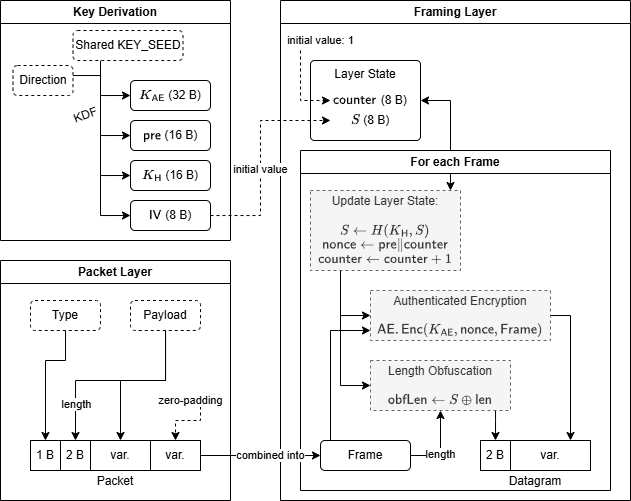
\includegraphics[width=\linewidth]{images/packet-framing.png}
    \caption[
        A visualization of \obfsfour{} framing at the sender.
    ]{
        A visualization of \obfsfour{} framing at the sender, where dashed shaded boxes correspond to subroutines, dashed unshaded boxes denote inputs, $\mathsf{AE}$ denotes the NaCl secretbox authenticated encryption scheme, and $H$ denotes the SipHash-2-4 pseudorandom function. 
    }
    \label{fig:framing}
\end{figure}

To create a packet, a packet type and the payload are required. The packet is then constructed and consists of the following:
\begin{itemize}
    \item A 1-byte packet type (corresponding to ``Payload'' or ``PrngSeed''),
    \item a 2-byte payload length in big endian format,
    \item the payload data itself, and
    \item configurable amounts of zero-padding (not included in the length calculation).
\end{itemize}

This packet is then passed on to a framing layer. While the packet layer ensures that a reliably received data stream can be decoded into separate variable-length messages with associated types, the framing layer's job is to encrypt, authenticate, and obfuscate the data.

For each direction, a counter value $\mathsf{counter}$ is initially set to 1, and a hash state $S$ is initialized to $\mathsf{IV}$.

For each frame (consisting of one or more packets) passed to the framing layer, several things occur:
\begin{enumerate}
    \item A nonce is computed as $ \mathsf{pre} \conc \mathsf{counter}$, and $\mathsf{counter}$ is incremented.
    \item One step of SipHash-2-4 in OFB mode is computed, yielding a fresh 8-byte hash state $S \gets H(K_\mathsf{H}, S)$.
\end{enumerate}

The entire packet is then encrypted using NaCl secretbox (Poly1305/XSalsa20) authenticated encryption with key $K_\mathsf{AE}$, producing a ciphertext; note that the ciphertext is longer than the packet payload, as padding and the secretbox overhead are now included.

The length of the ciphertext is then XORed with the first two bytes of the newly computed state $S$. The final datagram consists of:
\begin{itemize}
    \item A 2-byte obfuscated length field, and
    \item the AE ciphertext.
\end{itemize}

Upon receiving a packet, the receiver updates its $\mathsf{counter}$ and $S$ values, deobfuscated the length field, and decrypts the AE ciphertext. Finally, the data is passed up to the packet layer.

\paragraph{An Informal Security Analysis}

We will now discuss the achieved security guarantees by the above approach, to quickly survey possible improvements in future implementations.

The framing layer outlined above cannot, by design of the underlying Tor pluggable transport implementation, hide the length of transmitted frames from active attackers.
After the initial handshake, the connection is ``wrapped'' in the packet and framing layers, and for as long as the connections stay alive, data is passed back and forth between the local Tor client (in plaintext) and the bridge connection (encoded in packets).
If, at any point, a connection closes or raises an error (e.g. because a tag in the framing layer's AE ciphertext failed to verify), the connection is immediately closed, and a TCP FIN packet is sent by the OS as part of closing the TCP file descriptor.
This allows active attackers to choose any TCP burst after the initial handshake, leave the length field in the first two bytes unmodified, arbitrarily change the third byte (part of the 16 byte NaCl secretbox tag, ensuring a decryption failure later), and then slowly send one byte at a time. As the pluggable transport, after reading a valid length value, will wait for all data to arrive, and then verify the AE ciphertext, the total length of the AE ciphertext can be deduced by observing when the connection is closed.

This contrasts harshly with the handling of errors and invalid MAC values in the handshake procedure: There, a random delay between 1 and 60 seconds from the start of the connection is chosen as a deadline, and if a client causes an error in the handshake or does not send enough data in the first 30 seconds, the connection is closed only at this randomized deadline.

If active attackers attempt to fingerprint the connection by modifying the length value to provoke a closure of the connection (e.g. flipping the most significant bit, ensuring an invalid length), the length value is instead chosen as a random valid length between 16 to 1446 bytes. As the connection then remains blocked until the corresponding amount of AE ciphertext is received before the connection is closed, this attack cannot provoke a closure after a fixed, identifiable amount of data.

The main purpose of the length field obfuscation is therefore not to hide it from active attackers, or protect against manipulation (this is done by the authenticated encryption), but instead to make the protocol harder to identify. To this end, it is not clear to us, why $S$ is not instead chosen as e.g. $S \gets H(K_H, \mathsf{counter})$ to obtain a similarly secure random value to use in the XOR operation. This would remove the need for $\mathsf{IV}, S$ altogether and streamline the construction. Additionally, the \drivel{} PRF $F_1$ could be reused, reducing the number of primitives required in the protocol.

\paragraph{Design Conflicts and Conclusion}

To construct a system capable of flexible traffic shaping, it is necessary to split large messages into smaller ones, sent in sequence, as well as to pad small messages to a larger size, or even send only padding when no message is available.

The existing packet-based system in \obfsfour{} achieves exactly this, while providing authentication and side-stepping attacks from \cite{SP:AlbPatWat09}. Each packet incurs an overhead of 3 bytes plus configurable padding, and each frame (containing one or more packets, depending on the bridge configuration) adds 18 bytes.
The only precondition is a securely shared $\mathsf{KEY\_SEED}$.

It is possible to employ this system (possibly changing the employed schemes to match the security levels) directly in \drivel{}, using e.g. the early secret $ES$ after transmitting $c_S \conc A_C$ without encoding, and later switching to $\mathsf{KEY\_SEED}$ after the handshake is completed.

However, since the framing layer already aims to provide obfuscation, integrity, and confidentiality, the need for $P_C, M_C, \mathsf{MAC}_C, P_S, M_S, \mathsf{MAC}_S$ would disappear. Note that the message transcript is implicitly validated by including the $\mathsf{context}$ value when calculating $\mathsf{KEY\_SEED}$. Furthermore, it would not be necessary to encrypt $\pk_e$ at all.

We believe it to be worthwhile to modify \drivel{} accordingly, allowing almost arbitrary traffic shaping after an initial transmission of only $c_S \conc A_C$.
Conversely, this rather extensive change would require adapting the extensive $\sObfKE$ security proof for \drivel{} presented in \cite{EPRINT:GRSV25}.

This approach is visualized in \cref{fig:modified-drivel-framing}, an adaptation of \cite[Figure~6]{EPRINT:GRSV25}. Let $FL$ denote the framing layer presented above. Then $FL.\mathsf{Rekey}(k)$ indicates that the framing layer is reinitialized using $k$ as the $\mathsf{KEY\_SEED}$ value following the process outlined above.

\begin{figure}
    % \begin{minipage}[t]{\textwidth}
	\hfill
	\pseudocode[codesize=\footnotesize,jot=-1mm]{%
		\textbf{Server key generation/setup} \\
		\nodeid \getsr \bin^{\nodeidlen} \\
		(\pk_S, \sk_S) \getsr \OKEM.\kgen() \\
		\pstate.\macregister \gets \emptyset \\
		\text{return } ((\pk_S, \nodeid), (\sk_S, \nodeid), \pstate)
	}
	\hspace*{0.8cm}
% \end{minipage}

% \vspace{0.5em}

% \hspace*{-0.2in}
\centering
\scalebox{0.9}{%
\begin{tikzpicture}
	% Set the X coordinates of the client, server, and arrows
	\edef\ClientX{0}

	\edef\ArrowLeft{3}
	\edef\ArrowRight{13}
	\edef\ServerX{16.5}
	\edef\ServerLeftTextwidth{10.5cm} % width of server-side text, when left-aligned

	% Set the starting Y coordinate
	\edef\Y{0}

	% Draw header boxes
	\node [rectangle,draw,inner sep=5pt,right] at (\ClientX,\Y) {\textbf{Client}};
	\node [rectangle,draw,inner sep=5pt,left] at (\ServerX,\Y) {\textbf{Server}};
	
	\NextLine[0.4]
	\ClientAction[gray,font=\small]{\hspace{1.5cm}knows $(\pk_S, \nodeid)$}
	\ServerAction[gray,font=\small]{knows $(\sk_S, \nodeid)$\hspace{1.5cm}\null}
	\NextLine[1.1]
	
	\ClientAction{$(\pk_e, \sk_e) \getsr \KEM.\kgen()$} 
	\NextLine
	\ClientAction{$(c_S, K_S) \getsr \OKEM.\encaps(\pk_S)$}
	\NextLine
	\ClientAction{$ES \gets \funComb(\nodeid, K_S)$}
	\NextLine
	\ClientAction{$\mathsf{protoID} \gets \textlit{Drivel}$}
	\NextLine
	\ClientAction{\highlightbox{$\mathsf{context}_1 \gets \mathsf{protoID} \conc \pk_S \conc c_S$}}
	\NextLine
	\ClientAction{\highlightbox{$A_C \gets \funPRF(ES, \mathbf{H}(\mathsf{context}_1) \conc \textlit{:authc})$}}
	\NextLine
	\ClientAction{\highlightbox{$\mathsf{KEY\_SEED}_1 \gets \funPRF(ES, \mathbf{H}(\mathsf{context}_1) \| \textlit{:key\_extract\_1})$}}
	%%%%%%%%%%%%%%%%%%%%%%%%%%%%%%%%%%%%%%%%%%%%%%%%%%%%%%%%%%%%%%%%%%%%%%%%%%%%%%%%%%%%%%%%%%%%%%%%%%%%%%%
	\NextLine[2]
	\ClientToServer{\highlightbox{$\mathsf{msg}_C' = c_S \conc A_C$}}{}
	\NextLine
    %%%%%%%%%%%%%%%%%%%%%%%%%%%%%%%%%%%%%%%%%%%%%%%%%%%%%%%%%%%%%%%%%%%%%%%%%%%%%%%%%%%%%%%%%%%%%%%%%%%%%%%

    % Server verifies A_C and can start with dummy data
	\ServerActionLeft{$K_S \gets \OKEM.\decaps(\sk_S, c_S)$}
	\NextLine
	\ServerActionLeft{$ES \gets \funComb(\nodeid, K_S)$}
	\NextLine
	\ServerActionLeft{$\mathsf{protoID} \gets \textlit{Drivel}$}
	\NextLine
	\ServerActionLeft{\highlightbox{$\mathsf{context}_1 \gets \mathsf{protoID} \conc \pk_S \conc c_S$}}
	\NextLine
	\ServerActionLeft{\highlightbox{if $\funPRF(ES, \mathbf{H}(\mathsf{context}_1) \conc \textlit{:authc}) \neq A_C$: $\texttt{break}$}}
	\NextLine
	\ServerActionLeft{if \highlightbox{$A_C$}$ \in \pstate.\macregister$: $\texttt{break}$}
	\NextLine
	\ServerActionLeft{$\pstate.\macregister \gets \pstate.\macregister \cup $\highlightbox{$\{A_C\}$}}
	\NextLine
	\ServerActionLeft{\highlightbox{$\mathsf{KEY\_SEED}_1 \gets \funPRF(ES, \mathbf{H}(\mathsf{context}_1) \| \textlit{:key\_extract\_1})$}}
    %%%%%%%%%%%%%%%%%%%%%%%%%%%%%%%%%%%%%%%%%%%%%%%%%%%%%%%%%%%%%%%%%%%%%%%%%%%%%%%%%%%%%%%%%%%%%%%%%%%%%%%

    % Rekeying 1
    \NextLine
	\PhaseBreak{}{}
	\NextLine
    \ClientAction{\highlightbox{$FL.\mathsf{Rekey}(\mathsf{KEY\_SEED}_1)$}}
    \ServerAction{\highlightbox{$FL.\mathsf{Rekey}(\mathsf{KEY\_SEED}_1)$}}
    \NextLine[0.5]
	%%%%%%%%%%%%%%%%%%%%%%%%%%%%%%%%%%%%%%%%%%%%%%%%%%%%%%%%%%%%%%%%%%%%%%%%%%%%%%%%%%%%%%%%%%%%%%%%%%%%%%%

    % Start sending arbitrary data
	\ServerToClient[dashed,->]{}{}
	\ServerAction{\highlightbox{send arbitrary data}}
    %%%%%%%%%%%%%%%%%%%%%%%%%%%%%%%%%%%%%%%%%%%%%%%%%%%%%%%%%%%%%%%%%%%%%%%%%%%%%%%%%%%%%%%%%%%%%%%%%%%%%%%
    \NextLine[2]
	\ClientToServer{\highlightbox{$\mathsf{msg}_C'' = \pk_e$}}{}
	\NextLine
	%%%%%%%%%%%%%%%%%%%%%%%%%%%%%%%%%%%%%%%%%%%%%%%%%%%%%%%%%%%%%%%%%%%%%%%%%%%%%%%%%%%%%%%%%%%%%%%%%%%%%%%

    % Server parses rest of message and replies
    \ServerActionLeft{$(c_e, K_e) \getsr \KEM.\encaps(\pk_e)$}
	\NextLine
	\ServerActionLeft{$ES' \gets \funPRF(ES, \textlit{:derive\_key})$ ; $FS \gets \funComb(ES', K_e)$}
	\NextLine
	\ServerActionLeft{\highlightbox{$\mathsf{context}_2 \gets \mathsf{context}_1 \conc \pk_e \conc c_e$}}
	\NextLine
	\ServerActionLeft{$\mathsf{KEY\_SEED}_2 \gets \funPRF(FS, $\highlightbox{$\mathbf{H}(\mathsf{context}_2)$}$ \conc \textlit{:key\_extract\_2})$}
	\NextLine
	\ServerActionLeft{$\mathsf{auth} \gets \funPRF(FS, $\highlightbox{$\mathbf{H}(\mathsf{context}_2)$}$ \conc \textlit{:server\_mac})$}
	%%%%%%%%%%%%%%%%%%%%%%%%%%%%%%%%%%%%%%%%%%%%%%%%%%%%%%%%%%%%%%%%%%%%%%%%%%%%%%%%%%%%%%%%%%%%%%%%%%%%%%%
	\NextLine[1.5]
	\ServerToClient{\highlightbox{$\mathsf{msg}_S = c_e \conc \mathsf{auth}$}}{}
    %%%%%%%%%%%%%%%%%%%%%%%%%%%%%%%%%%%%%%%%%%%%%%%%%%%%%%%%%%%%%%%%%%%%%%%%%%%%%%%%%%%%%%%%%%%%%%%%%%%%%%%

    \NextLine
	\ClientAction{$K_e \gets \KEM.\decaps(\sk_e, c_e)$}
	\NextLine
	\ClientAction{$\mathsf{protoID} \gets \textlit{Drivel}$}
	\NextLine
	\ClientAction{$ES' \gets \funPRF(ES, \textlit{:derive\_key})$ ; $FS \gets \funComb(ES', K_e)$}
	\NextLine
	\ClientAction{\highlightbox{$\mathsf{context}_2 \gets \mathsf{context}_1 \conc \pk_e \conc c_e$}}
	\NextLine
	\ClientAction{$\mathsf{KEY\_SEED}_2 \gets \funPRF(FS, $\highlightbox{$\mathbf{H}(\mathsf{context}_2)$}$ \| \textlit{:key\_extract\_2})$}
	\NextLine
	\ClientAction{if $\funPRF(FS, $\highlightbox{$\mathbf{H}(\mathsf{context}_2)$}$ \conc \textlit{:server\_mac}) \neq \mathsf{auth}$: $\texttt{break}$}
    %%%%%%%%%%%%%%%%%%%%%%%%%%%%%%%%%%%%%%%%%%%%%%%%%%%%%%%%%%%%%%%%%%%%%%%%%%%%%%%%%%%%%%%%%%%%%%%%%%%%%%%

    % Rekeying 2
    \NextLine
	\PhaseBreak{}{}
	\NextLine
    \ClientAction{\highlightbox{$FL.\mathsf{Rekey}(\mathsf{KEY\_SEED}_2)$}}
    \ServerAction{\highlightbox{$FL.\mathsf{Rekey}(\mathsf{KEY\_SEED}_2)$}}
\end{tikzpicture}
}

    \caption[
        The modified \drivel{} protocol, simplified to take advantage of a framing layer.
    ]{
        The modified \drivel{} protocol, simplified to take advantage of a framing layer.
        $\OKEM$ is an OKEM satisfying $\indcca, \sprcca$ security, and ciphertext uniformity.
        $KEM$ is an $\indonecca$-secure KEM.
        $FL$ is a framing layer similar to the one described in \cref{sssec:variant-framing}.
        $F_1$ is a PRF and $F_2$ is a dual PRF.
        $\mathbf{H}$ is a collision-resistant hash function.
        Core differences to the \drivel{} protocol from \cite[Figure~6]{EPRINT:GRSV25} are highlighted in blue boxes.
        Messages are easily parsed due the the packet layer providing boundaries and the fixed-length components.
        A dashed arrow represents the option to send an arbitrary amount of uniformly random bits for the purpose of traffic shaping, e.g. by sending packets consisting only of padding.
        Dotted lines delimit the framing layer phases between $FL.\mathsf{Rekey}$ operations.
    }
    \label{fig:modified-drivel-framing}
\end{figure}

\paragraph{Note to Implementers and Future Work}

Should readers choose to implement or improve upon this proposed variant of \drivel{}, we encourage them to also consider the following items:

\begin{itemize}
    \item Calculating $\mathbf{H}(\mathsf{context}_2)$ can be done efficiently by reusing the hash state after digesting $\mathsf{context}_2$, avoiding the need to hash $\mathsf{context}_1$ twice. The hash outputs can be reused for two invocations of $F_1$ each time.
    
    \item This variant does not have a security proof like \drivel{}, and producing one would require formalizing the guarantees provided by the framing layer.

    \item As this thesis focuses on the key exchange phase, we did not propose improvements to the framing layer. However, previous work in this space exists \cite{Fenske2024} and should be considered to improve the framing layer from \obfsfour{}.

    \item Attention should be paid in particular to preventing modifications to the length fields (e.g. by authenticating them using fixed-length fields), and to handling errors consistently as discussed in the security analysis above and in \cite[Section~3.3]{Fenske2024}.

\end{itemize}

\section{Core Architecture} \label{sec:impl-architecture}
% TODO
% \Cref{sec:impl-architecture} describes how the protocol design was mapped to actual software components, including noteworthy architectural changes and cryptographic interfaces.

\paragraph{Building a KEM and OKEM from the \texttt{internal/x25519ell2} Module}

In the implementation of \obfsfour{}, only one method of key exchange is available: Customized Diffie-Hellman key exchange on the elliptic curve x25519, possibly using the \textsf{Elligator2} encoding on the curve points transmitted over the wire.

Post-quantum key-exchange algorithms are almost universally specified using the syntax of KEMs. In order to compare \drivel{} performance in the traditional setting with its performance using post-quantum KEMs, we have extended the \texttt{internal/x25519ell2} module to implement a KEM and a filter-encode obfuscator performing \textsf{Elligator2}. \Cref{fig:impl-x25519-kem} shows pseudocode illustrating the usage of the module by \obfsfour{} (through its use of the \texttt{common/ntor} module), alongside the construction of our x25519 KEM.

As our goal is simply to show how the KEM construction was extracted from the existing code, we omit the full definition of \obfsfour{} here. Suffice to say, the protocol involves one static keypair $\pk_\mathsf{id}, \sk_\mathsf{id}$ (the public key is part of the bridge information) and two ephemeral keypairs generated during the handshake procedure. The static keypair has no encodings applied to the public key (as it is transmitted out-of-band), while the ephemeral keypairs also have obfuscated public keys. When all required values are available, methods $\mathsf{ServerHandshake}, \mathsf{ClientHandshake}$ are executed to compute shared secrets which in turn are used to authenticate and finalize the handshake.

Readers should note that, although the construction is similar in spirit to the DHKEM construction \cite[Section~4.1]{rfc9180}, this KEM has minor differences in the derivation of its shared secret. Instead, the focus was on staying as close as possible to the construction used in \obfsfour{}, in order to offer a fair comparison between the two pluggable transport constructions when targeting traditional security.

Unlike in the \obfsfour{} protocol, the newly constructed KEM has what initially appear to be slightly different semantics to generate the obfuscated ciphertext $\hat \pk$:
In \obfsfour{} and its method $\mathsf{NewKeypair}$, the value $u$ determined by $\sk$ is passed directly to $\mathsf{uToRepresentative}$ whereas in the KEM, additional serialization ($\mathsf{Bytes}$) and deserialization ($\mathsf{SetBytes}$) takes place before $\mathsf{uToRepresentative}$ is invoked.
We have experimentally verified that this does not change $u$ and that the same $\hat \pk$ values are generated with both approaches, given the same randomness $t$.
Finally, the randomness $t$ is not taken from the hash function output used to set $\sk$, but rather generated securely on-the-fly. It is merely used for padding with two random bits, and to pick the sign of the curve point's y-coordinate at random as suggested in \cite{elligatorExplicitFormulas}.

\begin{figure}
    \begin{pchstack}[boxed, center, space=0.5em]

    \begin{pcvstack}[space=0.05em]
    % obfs4 usage via common/ntor
    \procedure[linenumbering]{Initialization}{
        \pclinecomment{$\pk_\mathsf{id}$ is part of the bridge information:} \\
        (\pk_\mathsf{id},\sk_\mathsf{id}) \getsr \mathsf{NewKeypair}(\mathsf{ell2}=0) \\
        \pclinecomment{upon the start of a new handshake:} \\
        (\pk_c,\sk_c) \getsr \mathsf{NewKeypair}(\mathsf{ell2}=1) \\
        (\pk_s,\sk_s) \getsr \mathsf{NewKeypair}(\mathsf{ell2}=1)
    }

    \procedure[linenumbering]{$\mathsf{NewKeypair}(\mathsf{ell2} \in \bin)$}{
        \pcdo \\
        \t  r \getsr \bin^{256} \\
        \t  d \gets \operatorname{\mathsf{SHA2-512}}(r) \\
        \t  \sk \gets \mathsf{firstBytes}(d,32) \\
        \t  \pcif \mathsf{ell2} = 1 \pcthen \\
        \t  \t  t \gets \mathsf{lastBytes}(d,1) \\
        \t  \t  \pclinecomment{inlined ScalarBaseMult(\sk, t)} \\
        \t  \t  u \gets \mathsf{scalarBaseMultDirty}(\sk) \\
        \t  \t  \pk \gets \mathsf{Bytes}(u) \\
        \t  \t  \hat \pk \gets \mathsf{uToRepresentative}(u, t) \\
        \t  \t  \pcif \pk \neq \bot \pcthen \\
        \t  \t  \t  \pcreturn (\pk, \hat \pk, \sk) \\
        \t  \t  \pcendif \\
        \t  \pcelse \\
        \t  \t  \pk \gets \mathsf{curve25519}.\mathsf{ScalarBaseMult}(\sk) \\
        \t  \t  \pcreturn (\pk, \bot, \sk) \\
        \t  \pcendif \\
        \pcwhile \pctrue
    }
   
    \procedure[lnstart=4,linenumbering]{$\mathsf{ServerHandshake}(\hat \pk_c, (\pk_s, \sk_s), (\pk_\mathsf{id},\sk_\mathsf{id}))$}{
        \pk_c \gets \mathsf{RepresentativeToPublicKey}(\hat \pk_c) \\
        K_1 \gets \mathsf{curve25519}.\mathsf{ScalarMult}(\sk_s, \pk_c) \\
        K_2 \gets \mathsf{curve25519}.\mathsf{ScalarMult}(\sk_\mathsf{id}, \pk_c) \\
        \pcif K_1 = 0 \lor K_2 = 0 \pcthen \pcabort \pcendif
    }
    
    \procedure[lnstart=4,linenumbering]{$\mathsf{ClientHandshake}((\pk_c, \sk_c), \hat \pk_s, \pk_\mathsf{id})$}{
        \pk_s \gets \mathsf{RepresentativeToPublicKey}(\hat \pk_s) \\
        K_1 \gets \mathsf{curve25519}.\mathsf{ScalarMult}(\sk_c, \pk_s) \\
        K_2 \gets \mathsf{curve25519}.\mathsf{ScalarMult}(\sk_c, \pk_\mathsf{id}) \\
        \pcif K_1 = 0 \lor K_2 = 0 \pcthen \pcabort \pcendif
    }
    \end{pcvstack}

    \begin{pcvstack}[space=0.05em]
    % KEM components
    \procedure[linenumbering]{$\KEM.\kgen()$}{
        r \getsr \bin^{256} \\
        d \gets \operatorname{\mathsf{SHA2-512}}(r) \\
        \sk \gets \mathsf{firstBytes}(d,32) \\
        u \gets \mathsf{scalarBaseMultDirty}(\sk) \\
        \pk \gets \mathsf{Bytes}(u) \\
        \pcreturn (\pk, \sk)
    }
   
    \procedure[lnstart=4,linenumbering]{$\KEM.\encaps(\pk)$}{
        \pk_e, \sk_e \getsr \kgen() \\
        K \gets \mathsf{curve25519}.\mathsf{ScalarMult}(\sk_e, \pk) \\
        \pcif K = 0 \pcthen \\
        \t  \pcabort \\
        \pcendif \\
        \pcreturn (c=\pk_e, K)
    }
    
    \procedure[lnstart=9,linenumbering]{$\KEM.\decaps(\sk, c)$}{
        u \gets \mathsf{SetBytes}(c) \\
        K \gets \mathsf{curve25519}.\mathsf{ScalarMult}(\sk, \mathsf{Bytes}(u)) \\
        \pcif K = 0 \pcthen \\
        \t  \pcabort \\
        \pcendif \\
        \pcreturn K
    }

    % FEO components
    \procedure[linenumbering]{$E.\filterpk(\pk)$}{
        \pclinecomment{no restriction on $\pk$ to encapsulate against} \\
        \pcreturn \pctrue
    }
    
    \procedure[lnstart=3,linenumbering]{$E.\encodectxt(c)$}{
        t \getsr \bin^{8} \\
        u \gets \mathsf{SetBytes}(c) \\
        \hat \pk \gets \mathsf{uToRepresentative}(u, t) \\
        \pclinecomment{$\hat \pk$ is $\bot$ for 50\% of all values of $c$} \\
        \pcreturn \hat \pk
    }
    
    \procedure[lnstart=5,linenumbering]{$E.\decodectxt(\hat c)$}{
        \pcreturn \mathsf{RepresentativeToPublicKey}(\hat c)
    }
    \end{pcvstack}

\end{pchstack}
    \caption[
        Pseudocode illustrating the x25519 KEM and filter-encode obfuscator added to the \texttt{internal/x25519ell2} module.
    ]{
        Pseudocode illustrating the x25519 KEM $\KEM$ and a filter-encode obfuscator $E$, both added to the \texttt{internal/x25519ell2} module.
        The left-hand side of the figure shows the usage of the x25519 module by \obfsfour{}, while the right-hand side defines a KEM and obfuscator for use in \drivel{}.
        The aborts identify insecure secrets caused by low-order public keys.
        We use $\mathsf{firstBytes}(x, \ell), \mathsf{lastBytes}(x, \ell)$ to denote selecting the first or last $\ell$ bytes of $x$, respectively.
        $\mathsf{curve25519}$ denotes the submodule of \texttt{golang.org/x/crypto} by the same name, all other functions are from the lyrebird repository's \texttt{internal/x25519ell2} and \texttt{common/ntor} modules.
    }
    \label{fig:impl-x25519-kem}
\end{figure}

\paragraph{Adding Crypto-Agility to the \texttt{internal} Module}

Observing the current need for post-quantum key exchange, combined with the increasing deployment of newly standardized algorithms, it seems prudent to implement at least compile-time flexibility in the utilized key exchange schemes. Being able to exchange cryptographic algorithms is often called ``being crypto-agile''.

To this end, the \drivel{} implementation contains string constants identifying the desired KEM and OKEM. The data structures for the schemes are then loaded at runtime based on these strings.
The schemes are identified by the following naming convention:
\begin{itemize}
    \item The string "x25519" refers to the unobfuscated, newly implemented KEM from \cref{fig:impl-x25519-kem},
    \item all other strings denote \texttt{liboqs} KEMs, and
    \item any KEM with a corresponding filter-encode obfuscator can be used to request an OKEM under the KEM name prefixed with ``FEO-'', e.g. ``FEO-x25519'' would denote $\feo[\KEM, E]$ using the components from \cref{fig:impl-x25519-kem}.
\end{itemize}

TODO: cryptofactory, kem/okem interfaces

\paragraph{Notable Differences between \texttt{transports/drivel} and \texttt{transports/obfs4}}

TODO: Implementation changes

\section{Deployment and Integration Guide} \label{sec:deployment}
% TODO
% \Cref{sec:deployment} provides practical guidance for the deployment and use of the system, with attention to real-world integration barriers.

% * How to deploy (same as lyrebird)
% * How to use (added pk files)
% * Integration barriers: Choosing KEM/OKEM, different SOCKS integration

\section{Challenges and Lessons Learned} \label{sec:challenges-learnings}
% TODO
% Finally, \cref{sec:challenges-learnings} discusses key challenges encountered during development and how they were addressed.

% * Having keys too large to derive HKDF key streams (8b counter not enough), switched to AES-CTR
% * Lack of client arguments to choose KEM/OKEM combination, requiring extra file for public keys
% * Note somewhere that we use the non-rejecting variant of Kemeleon
% * Debugging I-D for Kemeleon:
%    * https://github.com/rozbb/ct-kemeleon/blob/main/src/lib.rs#L69 does not implement SamplePreimage and directly encodes
%    * lists partial preimage equivalence sets https://github.com/jmwample/kemeleon/blob/main/src/kemeleon/ciphertext/precomputed.rs
%      we used these to improve SamplePreimage code. But does not have uniform distribution in https://github.com/jmwample/kemeleon/blob/main/src/kemeleon/ciphertext.rs#L150
% * Needing to hash the same data multiple times for different F_1 calls (luckily our choice of output length requires only one block ever)
\chapter{Experimental Evaluation}\label{ch:results}

\section{Experiment Setup} \label{sec:tbd}

* performance and traffic overhead compared to the original obfs4 protocol
* (efficacy of the protocol against blocking in censored regions)

\section{Measurement Results} \label{sec:tbd}

\section{Conclusions} \label{sec:tbd}

\chapter{Proposed Changes to the Protocol Design}\label{ch:protocol-changes}

For a definition of the \drivel{} protocol, as we implemented it in the course of this thesis, we refer readers to \cref{fig:drivel}, which served as our primary source.
This section dives into a theoretical discussion of proposed improvements to the protocol to better support traffic shaping and improve memory performance and suggests alternatives to \cref{fig:drivel}.
Future implementations may want to take inspiration from the ideas presented here to further improve \drivel{}.

\section{Discussion on Fragmenting Handshake Messages} \label{ssec:fragmentation}

This section analyzes possibilities to allow for more flexibility in shaping \drivel{} traffic. Avoiding fingerprinting based on certain sizes, directionalities and timing of messages between client and bridge is crucial to evade censors.

\textbf{No changes discussed or proposed in this \cref{ssec:fragmentation} were implemented, or practically evaluated as part of this thesis, but this discussion may be valuable to readers to understand possible future directions of the protocol.}

\paragraph{Fragmentation is Needed}
When deploying \drivel{}, it may be desirable to offer even more flexibility for traffic shaping than \obfsfour{}. In particular, \obfsfour{} sends two messages in its handshake, before fragmenting packets using a customizable message size distribution based on a deterministic pseudorandom number generator and a seed determined by the bridge server.

While \drivel{} also requires two messages to complete the handshake, \obfsfour{} messages range from 141 to 8~192 bytes in length, and \drivel{} message sizes depend on the selected KEM and OKEM. Ignoring the padding for the moment, \cref{tab:frag-msg-sizes} gives an overview of the minimum message sizes required for different combinations of KEM and OKEM in \drivel{}.

\begin{table}
    \centering \footnotesize
    \begin{tabular}{@{} L{0.2\textwidth-\tabcolsep} L{0.33\textwidth-2\tabcolsep} | L{0.3\textwidth-\tabcolsep} @{}}
    KEM with\newline Parameter Sets & OKEM with\newline Parameter Sets & Minimum Sizes (bytes)\newline Level 1 / Level 3 / Level 5 \\ \hline
    
    \multirow{4}{*}[-2.6em]{\shortstack[l]{ML-KEM\\ 512 / 768 / 1024}}
    & Classic-McEliece\newline 348864 / 460896 / 6688128\vspace{0.3em} & 928 / 1~372 / 1~808 \\
    & ML-Kemeleon\newline 512 / 768 / 1024\vspace{0.3em} & 1~709 / 2~468 / 3~258 \\
    & FEO-HQC\newline 128 / 192 / 256\vspace{0.3em} & 5~265 / 10~194 / 16~021 \\
    & FrodoKEM\newline 640 / 976 / 1344\vspace{0.3em} & 10~552 / 16~960 / 23~232 \\ \hline

    \multirow{4}{*}[-2.6em]{\shortstack[l]{BIKE\\ L1 / L3 / L5}}
    & Classic-McEliece\newline 348864 / 460896 / 6688128\vspace{0.3em} & 1~669 / 3~271 / 5~362 \\
    & ML-Kemeleon\newline 512 / 768 / 1024\vspace{0.3em} & 2~450 / 4~367 / 6~812 \\
    & FEO-HQC\newline 128 / 192 / 256\vspace{0.3em} & 6~006 / 12~093 / 19~575 \\
    & FrodoKEM\newline 640 / 976 / 1344\vspace{0.3em} & 11~293 / 18~859 / 26~786 \\ \hline

    \multirow{4}{*}[-2.6em]{\shortstack[l]{HQC\\ 128 / 192 / 256}}
    & Classic-McEliece\newline 348864 / 460896 / 6688128\vspace{0.3em} & 2~377 / 4~710 / 7~485 \\
    & ML-Kemeleon\newline 512 / 768 / 1024\vspace{0.3em} & 3~158 / 5~806 / 8~935 \\
    & FEO-HQC\newline 128 / 192 / 256\vspace{0.3em} & 6~714 / 13~532 / 21~698 \\
    & FrodoKEM\newline 640 / 976 / 1344\vspace{0.3em} & 12~001 / 20~298 / 28~909 \\ \hline

    \multirow{4}{*}[-2.6em]{\shortstack[l]{FrodoKEM\\ 640 / 976 / 1344}} 
    & Classic-McEliece\newline 348864 / 460896 / 6688128\vspace{0.3em} & 9~744 / 15~820 / 21~760 \\
    & ML-Kemeleon\newline 512 / 768 / 1024\vspace{0.3em} & 10~525 / 16~916 / 23~210 \\
    & FEO-HQC\newline 128 / 192 / 256\vspace{0.3em} & 14~081 / 24~642 / 35~973 \\
    & FrodoKEM\newline 640 / 976 / 1344\vspace{0.3em} & 19~368 / 31~408 / 43~184
    \end{tabular}
    \caption[
        Minimum sizes in bytes for the first \drivel{} message without padding depending on the choice of KEM and OKEM
    ]{
        Minimum sizes in bytes for the first \drivel{} message without padding depending on the choice of KEM and OKEM. Each cell contains minimum sizes for NIST security levels 1, 3, and 5.
        In the case of Classic McEliece, specific KEM parameter sets were selected to minimize message sizes while maintaining the targeted security level. The KEM parameter sets are identified in the first two columns.
    }
    \label{tab:frag-msg-sizes}
\end{table}

The concern in this section is that censors may observe particular traffic patterns. In particular, a bridge server never sends a reply before receiving the entire first \drivel{} or \obfsfour{} message in order to avoid probing attacks. This leads to quiet periods which may constitute an identifiable feature of the pluggable transport.

As is obvious from the table, sending the entire first \drivel{} message in full before the bridge responds (after verifying the PRF value at the end of message) leads to a large quiet period. Thus, for all but a few KEM/OKEM combinations, this quiet period would quickly be identifiable. At best, using Classic McEliece or ML-Kemeleon as an OKEM while employing ML-KEM or BIKE as a KEM would still yield sizes not exceeding 8~192 bytes, but the quiet periods would nonetheless be easy to distinguish from e.g.~\obfsfour{} traffic.

\paragraph{Desirable Security Properties}
Before discussing the options to mitigate this risk, let us recall one of the advantages \drivel{} has over \obfsfour{}. In \obfsfour{}, censors can retroactively identify handshake packets by verifying the MAC value if the bridge information is leaked, as the MAC it is keyed only with the bridge information. This allows censors to definitively identify clients that had previously connected to a bridge, as well as any future clients connecting to the bridge. This property has been discussed in \cite[Section~6]{CCS:GunSteVei24} and was also recognized earlier by David Fifield in \cite{obfs4-pk-reveal-distinguisher}.

Instead, \drivel{} establishes a shared secret between the client and the bridge in the first message. This shared secret is then used in addition to the bridge information to key the PRF. Censors therefore cannot retroactively identify obfuscated key exchanges with certainty, unless the OKEM private key is leaked. We will refer to this property here as \emph{strong obfuscation} ($\sObf$), as formally defined in \cite{CCS:GunSteVei24}.

For $\drivel$ to maintain its security, it is necessary that:
\begin{itemize}
    \item[a)] the bridge verifies the client's knowledge of the bridge information before sending a reply, and that
    \item[b)] the client's message proving this is indistinguishable from random bits, even given the bridge information and independent proofs from other clients.
\end{itemize}

Violating a) would make the bridge vulnerable to probing attacks by censors that do not know the bridge information. On the other hand, violating b) would trivially break $\sObf$. Both of these outcomes would be undesirable and $\sObfKE$ from \cite{CCS:GunSteVei24} captures both avenues of attack, since the predicate \textsf{Probed} automatically wins the game, and public keys can be revealed when asked to distinguish a simulated transcript from a real transcript in \textsc{ChallExec}, respectively.

Due to the required proof in the client's initial communication alone, it is strictly necessary that the bridge server receives a certain minimum amount of data before it may respond in any way.
To break up the first large \drivel{} message, we could, for example, split it into parts and let the server respond after receiving each of these smaller parts. However, the first such ``fragment'' would need to contain at least a suitable proof that the client knows the bridge information.

\paragraph{An Informal Security Notion}
In order to outline the above requirements a bit more, we can informally define the initial interaction between an adversary and the bridge servers. One goal of the initial exchange, among others, is to arrive at a shared secret, that can aid in subsequent fragmentation, using just the first message from the client to the server.

This effectively means that a first fragment could be viewed as an (O)KEM ciphertext: Some bridge information is generated and distributed (similar to a public key), a message is sent by a client to the bridge and a shared secret is computed from it.
% Conversely, the first fragment may also be viewed as a MAC tag: Bridge information is then assumed to be secret and shared between two parties (similar to a symmetric key), and used to authenticate a communication.

Let us also assume that there is no possibility for bridges to save state about each client, that clients are unwilling to save state for the bridges due to privacy concerns (both options could be implemented e.g. similar to TLS 1.3 session resumption \cite[Section~2.2]{rfc8446}) and that no pre-shared symmetric keys are available (which would trivialize the entire handshake).

For the following discussion, let $P$ be the bridge information.
Let $M$ denote the fixed-length message sent from the client to the bridge, and let $S$ denote the shared secret computed by both client and bridge for the secure transport of subsequent traffic.
% We also define two adversaries $\adv$ and $\bdv$. The bridge information $P$ is only known to $\adv$, and not $\bdv$.
We also define an adversary $\adv$, to which the bridge information $P$ is known.
The goal of $\adv$ is to identify traffic as a client-bridge handshake (breaking strong obfuscation).
% and $\bdv$ attempts to elicit a response from a bridge (breaking probing resistance).

We will now examine what properties (in addition to probing resistance) this exchange should satisfy:
\begin{itemize}
    \item The adversary $\adv$ should not be able to distinguish the first fragment sent over the network from random bits, even given $P$ (e.g. retroactively). This corresponds directly to $\ctxtunif$, if we were to view the exchange as an OKEM.

    \item The adversary $\adv$ should not be able to distinguish a randomly sampled shared secret $S$ from one corresponding to any given message $M$ observed on the network, even if the adversary is allowed further communication with the bridge. Viewing the exchange as a KEM, this corresponds to $\indcca$ security.
    
    % \item The adversary $\bdv$ should not be able to create a message $M$ that, when parsed by the bridge results in a valid shared secret $S$ without access to the bridge information. This would allow bridges to respond, violating probing resistance. Instead, the bridge should reject the message. Here, we can view the exchange as a MAC application using the previously shared bridge information $P$ as a key. The property then corresponds to the standard notion of strongly secure MACs as defined in \cite[Definition~4.3]{katz_lindell}, \cite[Chapter~2]{AC:BelNam00}.
\end{itemize}

Note also that in the case of \drivel{}, without any modifications discussed below, these properties are achieved when choosing $M$ to be the entire first protocol message:
% The first two requirements are covered by the OKEM, and the last property is achieved by authenticating every message with a PRF value.
The OKEM covers both requirements, and probing resistance is also achieved by authenticating every message with a PRF value.

It is hard to imagine a significant potential in message size reduction outside of removing other components of the first \drivel{} message, as we conjecture the following:
Any protocol satisfying the requirements listed above could act as an OKEM.
%(or an inefficient MAC).
The existence of a more efficient protocol would thus imply the existence of a more efficient OKEM, which, due to the large scope of the NIST Standardization \cite{nist-standardization}, seems implausible.
This gives us confidence that both the constructions in \cref{ssec:drivel-mod} below are close to optimal in terms of the size of the first fragment.

\paragraph{Arbitrary Fragmentation}
We have focused on maintaining $\sObf$ security during fragmentation up until now, as this was also a design goal for \drivel{}.
If, however, compromises could be made in regards to $\sObf$ security, the fragmentation would not suffer the constraints outlined above.

Relaxing our requirements, and allowing a censor to retroactively identify bridges given their bridge information, the following fragmentation strategy becomes reasonable: The client sends a first fragment of $x+16$ bytes, consisting only of $x$ bytes of uniformly random data and a 16 byte PRF keyed with the bridge information. Padding may be added between the two blocks. The choice of $x$ does not impact the security, but reduces the chance of bridges rejecting honest connection attempts due to repeated PRF values.

The rejection of repeated PRF values works using ``epoch hours'', i.e. the number of seconds since the Unix epoch divided by 60.
The current epoch hour is used as an input to every PRF calculation, and verifiers only accept PRF values that used an epoch hour not different from their local value by more than 1.
This allows bridges to partially clear the set of already received PRF values (used to prevent replay attacks checks) every hour.
In particular, the value of $x$ must be such that the chance of collisions in those $x$ bytes must be kept small within a given epoch hour.

As an example, \cite{tor-metrics} reports around 112~000 users across all pluggable transports and around 1~900 bridges, so assuming an even distribution of users across bridges, this would mean an average of 60 active users per bridge, each making at most 60 handshakes per epoch hour. Using those numbers, choosing $x=6$ already yields a collision probability $\leq 3 \cdot 10^{-8}$ by the birthday bound (with $2^{48}$ possible values and only $2^{11.8}$ samples per epoch hour).

This approach is very similar in spirit to the first message in \obfsfour{} (in that it does not use a shared secret in the calculation of the PRF value) and allows for much more flexibility in traffic shaping through padding. The key difference from \obfsfour{} is the removal of one of the PRF values and the aggressive reduction in message size by replacing the obfuscated client public key with randomized data.

If implementations are willing to accept some additional complexity, these $x$ bytes of uniformly random data might also be replaced with the start of any key exchange message that would be sent after this initial message (e.g. the first $x$ bytes of $\mathsf{epk}_e$ in the case of \drivel{}). This would achieve the same effect of proving that the client knows the bridge information as soon as possible, as long as collisions in the first $x$ bytes are sufficiently unlikely.

Sending even less data in a first fragment seems implausible, as the randomized data is necessary to prevent replay attacks while avoiding false positives, and the PRF value proves knowledge of the bridge information. Using less than $x$ or 16 bytes, respectively, for either component would lower the security level or increase the collision probability between users, forcing handshake retries.

\section{Proposed Modifications to the Drivel Protocol} \label{ssec:drivel-mod}

No changes discussed or proposed in this \cref{ssec:drivel-mod} were implemented or practically evaluated as part of this thesis, but this discussion may be valuable to readers to understand possible future directions of the protocol.

This thesis employs only the unmodified variant of $\drivel{}$ presented in \cref{fig:drivel}.

The following two subsections offer different approaches to implement fragmentation of handshake messages in \drivel{}. \Cref{sssec:variant-minimal} tries to make only small changes to \drivel{}, as proposed in \cref{fig:drivel}, while \cref{sssec:variant-framing} tries to reuse existing mechanisms in \obfsfour{} and extend them from the data transfer to the handshake phase.

\subsection{Variant 1: A Minimal Fragmentation} \label{sssec:variant-minimal}

One way to achieve the security properties described in \cref{ssec:fragmentation} in a space-efficient manner would be to send one OKEM ciphertext plus a 16 byte PRF value as the first fragment. The PRF would be keyed by a combination of the shared secret and the bridge information (as in \drivel{}).

Recall from \cref{fig:drivel} that the first \drivel{} message is constructed as $\mathsf{epk}_e \conc c_S \conc P_C \conc M_C \conc \mathsf{MAC}_C$, where $\mathsf{epk}_e$ is the encrypted KEM public key, $c_S$ is the OKEM ciphertext of interest, $M_C$ helps delimit the message, and $\mathsf{MAC}_C$ authenticates all preceding data.

In this fragmentation approach, we propose a minimal change to this message, such that encrypted public keys $\mathsf{epk}_e$ are sent later, and an additional PRF value (the ``authenticator'') is sent directly following the OKEM ciphertext. Reusing the same variables, parenthesizing the first fragment for clarity, and introducing $A_C \gets F_1(ES, c_S \conc \text{``:authc''})$ as an authenticator, this would lead to the following first protocol message:

\[
    \left( c_S \conc A_C \right) \conc \mathsf{epk}_e \conc P_C \conc M_C \conc \mathsf{MAC}_C .
\]

Using this modified first message, the bridge may now start sending data earlier than in unmodified \drivel{}. Although it cannot send its second message before receiving $\mathsf{epk}_e$, it can send dummy data that the client will ignore.

The adapted protocol specification is visualized in \cref{fig:modified-drivel-minimal}, an adaptation of \cref{fig:drivel}. Dashed lines denote the option to send dummy data for the purpose of traffic shaping.

\begin{figure}
    % \begin{minipage}[t]{\textwidth}
	\hfill
	\pseudocode[codesize=\footnotesize,jot=-1mm]{%
		\textbf{Server key generation/setup} \\
		\nodeid \getsr \bin^{\nodeidlen} \\
		(\pk_S, \sk_S) \getsr \OKEM.\kgen() \\
		\pstate.\macregister \gets \emptyset \\
		\text{return } ((\pk_S, \nodeid), (\sk_S, \nodeid), \pstate)
	}
	\hspace*{0.8cm}
% \end{minipage}

% \vspace{0.5em}

% \hspace*{-0.2in}
\centering
\scalebox{0.77}{%
\begin{tikzpicture}
	% Set the X coordinates of the client, server, and arrows
	\edef\ClientX{0}

	\edef\ArrowLeft{3}
	\edef\ArrowRight{13}
	\edef\ServerX{16.5}
	\edef\ServerLeftTextwidth{10.5cm} % width of server-side text, when left-aligned

	% Set the starting Y coordinate
	\edef\Y{0}

	% Draw header boxes
	\node [rectangle,draw,inner sep=5pt,right] at (\ClientX,\Y) {\textbf{Client}};
	\node [rectangle,draw,inner sep=5pt,left] at (\ServerX,\Y) {\textbf{Server}};
	
	\NextLine[0.4]
	\ClientAction[gray,font=\small]{\hspace{1.5cm}knows $(\pk_S, \nodeid)$}
	\ServerAction[gray,font=\small]{knows $(\sk_S, \nodeid)$\hspace{1.5cm}\null}
	\NextLine[1.1]
	
	\ClientAction{$(\pk_e, \sk_e) \getsr \KEM.\kgen()$} 
	\NextLine
	\ClientAction{$P_C \getsr \mathcal{D}_{\mathsf{pad}_C}$}
	\NextLine
	\ClientAction{$(c_S, K_S) \getsr \OKEM.\encaps(\pk_S)$}
	\NextLine
	\ClientAction{$ES \gets \funComb(\nodeid, K_S)$}
	\NextLine
	\ClientAction{$EK_1 \gets \funPRF(ES, \textlit{:enckey1}, \keylen_1)$}
	\NextLine
	\ClientAction{$EK_2 \gets \funPRF(ES, \textlit{:enckey2}, \keylen_2)$}
	\NextLine
	\ClientAction{$\mathsf{epk}_e \gets \funEnc(EK_1, \pk_e)$}
	\NextLine
	\ClientAction{\highlightbox{$A_C \gets \funPRF(ES, c_S \conc \textlit{:authc})$}}
    \NextLine
	\ClientAction{\highlightbox{$A_S \gets \funPRF(ES, \textlit{:auths})$}}
	\NextLine
	\ClientAction{$M_C \gets \funPRF(ES, \mathsf{epk}_e \conc \textlit{:mc})$}
	\NextLine
	\ClientAction{$\mathsf{MAC}_C \gets \funPRF(ES,$\highlightbox{$c_S \conc A_C \conc \mathsf{epk}_e$}$\conc P_C \conc M_C \conc \textlit{:mac\_c})$}
	%%%%%%%%%%%%%%%%%%%%%%%%%%%%%%%%%%%%%%%%%%%%%%%%%%%%%%%%%%%%%%%%%%%%%%%%%%%%%%%%%%%%%%%%%%%%%%%%%%%%%%%
	\NextLine[2]
	\ClientToServer{\highlightbox{$\mathsf{msg}_C' = c_S \conc A_C$}}{}
	\NextLine
    %%%%%%%%%%%%%%%%%%%%%%%%%%%%%%%%%%%%%%%%%%%%%%%%%%%%%%%%%%%%%%%%%%%%%%%%%%%%%%%%%%%%%%%%%%%%%%%%%%%%%%%

    % Server verifies A_C and can start with dummy data
    \ServerActionLeft{$c_S \gets \mathsf{msg}_C'[1..\obfctxtlen]$ ; \highlightbox{$A_C \gets \mathsf{msg}_C'[\obfctxtlen+1..\obfctxtlen+\funPRFoutlen]$}}
	\NextLine
	\ServerActionLeft{$K_S \gets \OKEM.\decaps(\sk_S, c_S)$}
	\NextLine
	\ServerActionLeft{$ES \gets \funComb(\nodeid, K_S)$}
	\NextLine
	\ServerActionLeft{$EK_1 \gets \funPRF(ES, \textlit{:enckey1}, \keylen_1)$}
	\NextLine
	\ServerActionLeft{$EK_2 \gets \funPRF(ES, \textlit{:enckey2}, \keylen_2)$}
	\NextLine
	\ServerActionLeft{\highlightbox{if $\funPRF(ES, c_S \conc \textlit{:authc}) \neq A_C$: $\texttt{break}$}}
	\NextLine
	\ServerActionLeft{if \highlightbox{$A_C$}$ \in \pstate.\macregister$: $\texttt{break}$}
	\NextLine
	\ServerActionLeft{$\pstate.\macregister \gets \pstate.\macregister \cup $\highlightbox{$\{A_C\}$}}
    \NextLine
	\ServerActionLeft{\highlightbox{$A_S \gets \funPRF(ES, \textlit{:auths})$}}
    %%%%%%%%%%%%%%%%%%%%%%%%%%%%%%%%%%%%%%%%%%%%%%%%%%%%%%%%%%%%%%%%%%%%%%%%%%%%%%%%%%%%%%%%%%%%%%%%%%%%%%%
    \NextLine[0.5]
	\ServerToClient[dashed,->]{}{}
	%%%%%%%%%%%%%%%%%%%%%%%%%%%%%%%%%%%%%%%%%%%%%%%%%%%%%%%%%%%%%%%%%%%%%%%%%%%%%%%%%%%%%%%%%%%%%%%%%%%%%%%

    % Client waits for A_S
	\ServerAction{\highlightbox{send arbitrary data}}
    \ClientAction{\highlightbox{discard until $A_S$}}
    %%%%%%%%%%%%%%%%%%%%%%%%%%%%%%%%%%%%%%%%%%%%%%%%%%%%%%%%%%%%%%%%%%%%%%%%%%%%%%%%%%%%%%%%%%%%%%%%%%%%%%%
    \NextLine[1.2]
	\ClientToServer{$\mathsf{msg}_C'' = $\highlightbox{$\mathsf{epk}_e \conc P_C$}$ \conc M_C \conc \mathsf{MAC}_C$}{}
	\NextLine
	%%%%%%%%%%%%%%%%%%%%%%%%%%%%%%%%%%%%%%%%%%%%%%%%%%%%%%%%%%%%%%%%%%%%%%%%%%%%%%%%%%%%%%%%%%%%%%%%%%%%%%%

    % Server parses rest of message and replies
    \ServerActionLeft{$\mathsf{epk}_e \gets \mathsf{msg}_C''[1..\pklen]$}
	\NextLine
	\ServerActionLeft{$M_C \gets \funPRF(ES, \mathsf{epk}_e \conc \textlit{:mc})$}
	\NextLine
	\ServerActionLeft{parse $(\mathsf{epk}_e \conc P_C \conc M_C \conc \mathsf{MAC}_C) \gets \mathsf{msg}_C''$ using $M_C$; else $\texttt{break}$}
	\NextLine
	\ServerActionLeft{if $\funPRF(ES,$\highlightbox{$c_S \conc A_C \conc \mathsf{epk}_e$}$\conc P_C \conc M_C \conc \textlit{:mac\_c}) \neq \mathsf{MAC}_C$: $\texttt{break}$}
	\NextLine
	\ServerActionLeft{$\pk_e \gets \funDec(EK_1, \mathsf{epk}_e)$}
	\NextLine
	\ServerActionLeft{$(c_e, K_e) \getsr \KEM.\encaps(\pk_e)$}
	\NextLine
	\ServerActionLeft{$\mathsf{ect}_e \gets \funEnc(EK_2, c_e)$}
	\NextLine
	\ServerActionLeft{$\mathsf{protoID} \gets \textlit{Drivel}$}
	\NextLine
	\ServerActionLeft{$ES' \gets \funPRF(ES, \textlit{:derive\_key})$ ; $FS \gets \funComb(ES', K_e)$}
	\NextLine
	\ServerActionLeft{$\mathsf{context} \gets \pk_S \conc c_S \conc \pk_e \conc c_e \conc \mathsf{protoID}$}
	\NextLine
	\ServerActionLeft{$\mathsf{KEY\_SEED} \gets \funPRF(FS, \mathsf{context} \conc \textlit{:key\_extract})$}
	\NextLine
	\ServerActionLeft{$\mathsf{auth} \gets \funPRF(FS, \mathsf{context} \conc \textlit{:server\_mac})$}
	\NextLine
	\ServerActionLeft{$P_S \getsr \mathcal{D}_{\mathsf{pad}_S}$}
	\NextLine
	\ServerActionLeft{$M_S \gets \funPRF(ES, \mathsf{ect}_e \conc \textlit{:ms})$}
	\NextLine
	\ServerActionLeft{$\mathsf{MAC}_S \gets \funPRF(ES,$\highlightbox{$A_S$}$\conc \mathsf{ect}_e \conc \mathsf{auth} \conc P_S \conc M_S \conc \textlit{:mac\_s})$}
	
	%%%%%%%%%%%%%%%%%%%%%%%%%%%%%%%%%%%%%%%%%%%%%%%%%%%%%%%%%%%%%%%%%%%%%%%%%%%%%%%%%%%%%%%%%%%%%%%%%%%%%%%
	\NextLine[1.5]
	\ServerToClient{$\mathsf{msg}_S =$\highlightbox{$A_S$}$\conc \mathsf{ect}_e \conc \mathsf{auth} \conc P_S \conc M_S \conc \mathsf{MAC}_S$}{}
	\NextLine
	%%%%%%%%%%%%%%%%%%%%%%%%%%%%%%%%%%%%%%%%%%%%%%%%%%%%%%%%%%%%%%%%%%%%%%%%%%%%%%%%%%%%%%%%%%%%%%%%%%%%%%%
	
	\ClientAction{$\mathsf{ect}_e \gets \mathsf{msg}_S[1..\ctxtlen]$}
	\NextLine
	\ClientAction{$M_S \gets \funPRF(ES, \mathsf{ect}_e \conc \textlit{:ms})$}
	\NextLine
	\ClientAction{parse $(\mathsf{ect}_e \conc \mathsf{auth} \conc P_S \conc M_S \conc \mathsf{MAC}_S) \gets \mathsf{msg}_S$ using $M_S$; else $\texttt{break}$}
	\NextLine
	\ClientAction{if $\funPRF(ES,$\highlightbox{$A_S$}$\conc \mathsf{ect}_e \conc \mathsf{auth} \conc P_S \conc M_S \conc \textlit{:mac\_s}) \neq \mathsf{MAC}_S$: $\texttt{break}$}
	\NextLine
	\ClientAction{$c_e \gets \funDec(EK_2, \mathsf{ect}_e)$}
	\NextLine
	\ClientAction{$K_e \gets \KEM.\decaps(\sk_e, c_e)$}
	\NextLine
	\ClientAction{$\mathsf{protoID} \gets \textlit{Drivel}$}
	\NextLine
	\ClientAction{$ES' \gets \funPRF(ES, \textlit{:derive\_key})$ ; $FS \gets \funComb(ES', K_e)$}
	\NextLine
	\ClientAction{$\mathsf{context} \gets \pk_S \conc c_S \conc \pk_e \conc c_e \conc \mathsf{protoID}$}
	\NextLine
	\ClientAction{$\mathsf{KEY\_SEED} \gets \funPRF(FS, \mathsf{context} \| \textlit{:key\_extract}) $}
	\NextLine
	\ClientAction{if $\funPRF(FS, \mathsf{context} \conc \textlit{:server\_mac}) \neq \mathsf{auth}$: $\texttt{break}$}
\end{tikzpicture}
}

    \caption[
        The modified \drivel{} protocol, with minimal changes to support fragmentation.
    ]{
        The modified \drivel{} protocol, with minimal changes to support fragmentation.
        $\OKEM$ is an OKEM satisfying $\indcca, \sprcca$ security, and ciphertext uniformity.
        $KEM$ is an $\indonecca$-secure KEM.
        $SE$ is a length-preserving, one-time ciphertext indistinguishable, symmetric encryption scheme.
        $F_1$ is a PRF and $F_2$ is a dual PRF.
        Core differences to the \drivel{} protocol from \cref{fig:drivel} are highlighted in blue boxes.
        A dashed arrow represents the option to send an arbitrary amount of uniformly random bits for the purpose of traffic shaping.
    }
    \label{fig:modified-drivel-minimal}
\end{figure}

Implementers should note that the newly introduced $A_C$ must be saved to protect against replay attacks. This replaces the existing replay protection in \obfsfour{} which uses $\mathsf{MAC}_C$. The same mechanism can be reused.

There is no need to check for repeats between $\mathsf{MAC}_C$ values in this variant. The goal of these checks is to prevent the server from answering on replayed messages, in order to resist active probing.
However, replayed messages by definition also contain the same value for $A_C$ and would be rejected even earlier.

\Cref{tab:frag-min-needed} shows the minimum size of a first fragment using this approach for different OKEMs. Note that this is simply the size of OKEM ciphertexts plus 16 bytes for the PRF value.

\begin{table}
    \centering \small
    \begin{tabular}{@{} L{0.1\textwidth-\tabcolsep} | R{0.3\textwidth-2\tabcolsep} R{0.2\textwidth-2\tabcolsep} R{0.2\textwidth-2\tabcolsep} R{0.2\textwidth-\tabcolsep} @{}}
        & Classic-McEliece\newline \footnotesize 348864 / 460896 / 6688128
        & ML-Kemeleon\newline 512 / 768 / 1024
        & FEO-HQC\newline 128 / 192 / 256
        & FrodoKEM\newline 640 / 976 / 1344
        \\ \hline
    Level 1 & 112 & 893 & 4~449 & 9~736 \\
    Level 3 & 172 & 1~268 & 8~994 & 15~760 \\
    Level 5 & 224 & 1~674 & 14~437 & 21~648
    \end{tabular}
    \caption[
        Minimum sizes in bytes of a first fragment before a bridge may respond depending on the choice of OKEM.
    ]{
        Minimum sizes in bytes of a first fragment before a bridge may respond depending on the choice of OKEM. Rows denote NIST security levels. Parameter sets were selected to minimize message sizes while maintaining the targeted security level. The KEM parameter sets are identified in the row and column headers.
    }
    \label{tab:frag-min-needed}
\end{table}

It follows that using Classic McEliece or ML-Kemeleon as OKEMs allows for the most freedom in choosing message sizes. Using HQC quickly produces large ciphertexts for higher security levels.

Once this first fragment has been received by the server, later fragmentation does not suffer from the same size constraints, as the use of the shared secret then effectively proves that the client knows the bridge information and that the bridge holds the OKEM private key. Exchanging almost arbitrarily small fragments becomes feasible by simply authenticating them using the shared secret and a PRF.

\subsection{Variant 2: Reusing \obfsfour{} Framing} \label{sssec:variant-framing}

\paragraph{Existing Fragmentation Mechanisms in obfs4}
The lyrebird repository's \obfsfour{} implementation features a packet-based system capable of transferring different types of messages during the data transfer phase. This system could be reused to implement more flexible fragmentation after the initial fragment $c_S \conc A_C$ is transmitted, but its construction duplicates part of the \drivel{} protocol.

At the time of writing, this packet-based system can be outlined as follows. Given a securely established shared secret $\mathsf{KEY\_SEED}$, both client and bridge derive two sets of the following values from it:
\begin{itemize}
    \item A 32-byte authenticated encryption (AE) key $K_\mathsf{AE}$,
    \item a 16-byte nonce prefix $\mathsf{pre}$,
    \item a 16-byte hash key $K_\mathsf{H}$, and
    \item an 8-byte hash IV $\mathsf{IV}$.
\end{itemize}

Each set of $K_\mathsf{AE}, \mathsf{pre}, K_\mathsf{H}, \mathsf{IV}$ corresponds to either the direction client-to-bridge, or bridge-to-client. Both directions work in the same way presented below and visualized in \cref{fig:framing}.

\begin{figure}
    \centering
    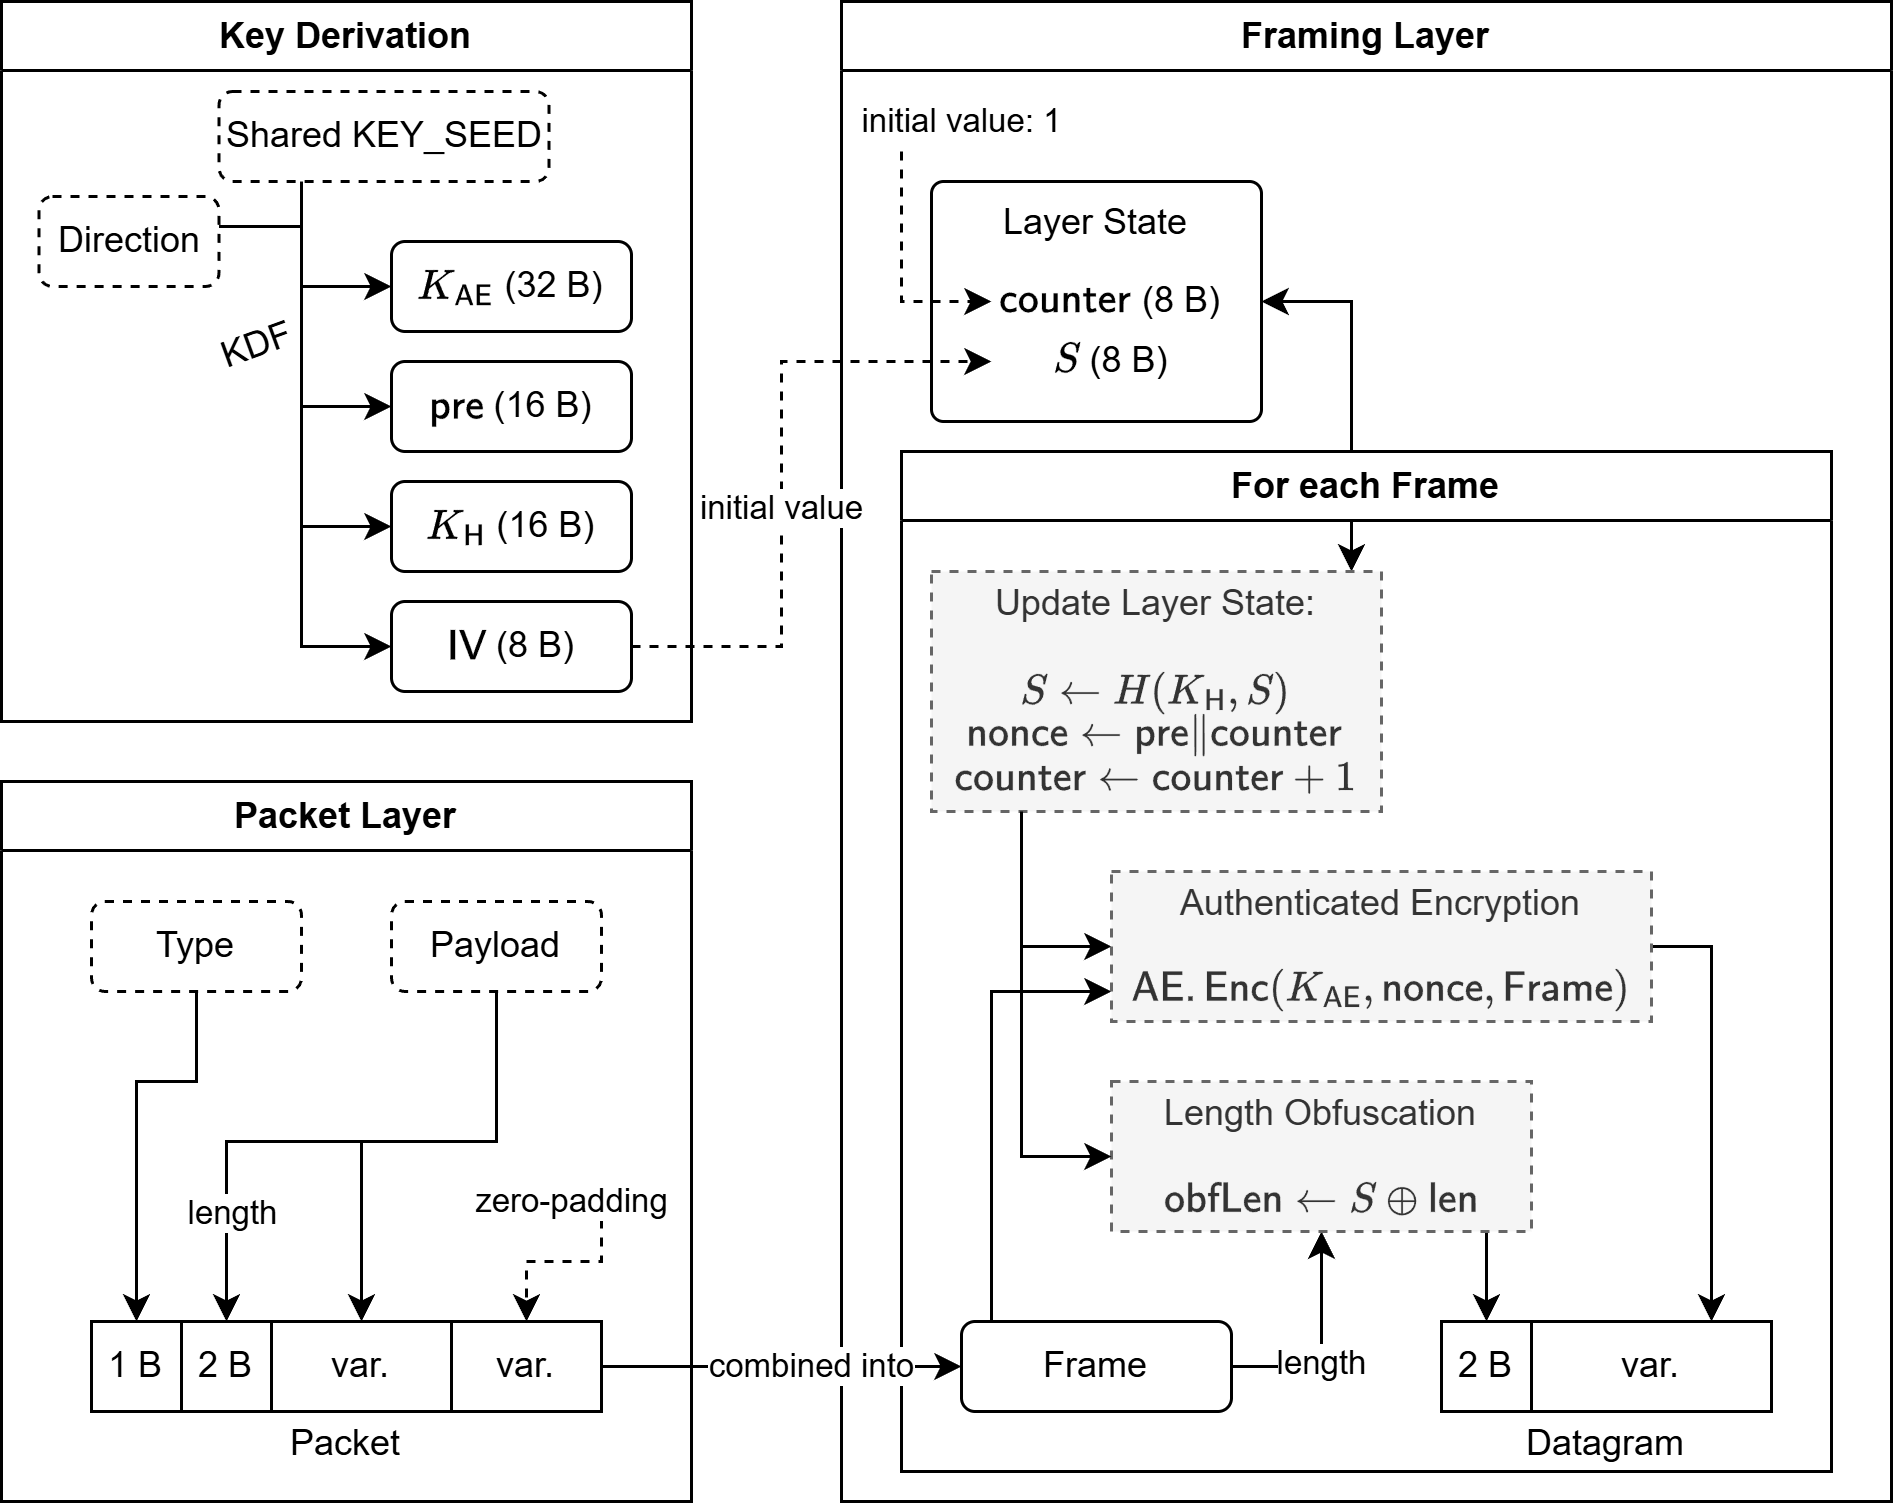
\includegraphics[width=\linewidth]{images/packet-framing.drawio.png}
    \caption[
        A visualization of \obfsfour{} framing at the sender.
    ]{
        A visualization of \obfsfour{} framing at the sender, where dashed shaded boxes correspond to subroutines, dashed unshaded boxes denote inputs, $\mathsf{AE}$ denotes the NaCl secretbox authenticated encryption scheme, and $H$ denotes the SipHash-2-4 pseudorandom function.
    }
    \label{fig:framing}
\end{figure}

To create a packet, a packet type and the payload are required. The packet is then constructed and consists of the following:
\begin{itemize}
    \item A 1-byte packet type (corresponding to ``Payload'' or ``PrngSeed''),
    \item a 2-byte payload length in big endian format,
    \item the payload data itself, and
    \item configurable amounts of zero-padding (not included in the length calculation).
\end{itemize}

This packet is then passed on to a framing layer. While the packet layer ensures that a reliably received data stream can be decoded into separate variable-length messages with associated types, the framing layer's job is to encrypt, authenticate, and obfuscate the data.

For each direction, a counter value $\mathsf{counter}$ is initially set to 1, and a hash state $S$ is initialized to $\mathsf{IV}$.

For each frame (consisting of one or more packets) passed to the framing layer, several things occur:
\begin{enumerate}
    \item A nonce is computed as $ \mathsf{pre} \conc \mathsf{counter}$, and $\mathsf{counter}$ is incremented.
    \item One step of SipHash-2-4 in OFB mode is computed, yielding a fresh 8-byte hash state $S \gets H(K_\mathsf{H}, S)$.
\end{enumerate}

The entire packet is then encrypted using NaCl secretbox (Poly1305/XSalsa20) authenticated encryption with key $K_\mathsf{AE}$, producing a ciphertext; note that the ciphertext is longer than the packet payload, as padding and the secretbox overhead are now included.

The length of the ciphertext is then XORed with the first two bytes of the newly computed state $S$. The final datagram consists of:
\begin{itemize}
    \item A 2-byte obfuscated length field, and
    \item the AE ciphertext.
\end{itemize}

Upon receiving a packet, the receiver updates its $\mathsf{counter}$ and $S$ values, de-obfuscates the length field, and decrypts the AE ciphertext. Finally, the data is passed up to the packet layer.

\paragraph{An Informal Security Analysis}

We will now discuss the achieved security guarantees by the above approach, to quickly survey possible improvements in future implementations.

The framing layer outlined above cannot, by design of the underlying Tor pluggable transport implementation, hide the length of transmitted frames from active attackers.
After the initial handshake, the connection is ``wrapped'' in the packet and framing layers, and for as long as the connections stay alive, data is passed back and forth between the local Tor client (in plaintext) and the bridge connection (encoded in packets).
If, at any point, a connection closes or raises an error (e.g. because a tag in the framing layer's AE ciphertext failed to verify), the connection is immediately closed, and a TCP FIN packet is sent by the OS as part of closing the TCP file descriptor.
This allows active attackers to choose any TCP burst after the initial handshake, leave the length field in the first two bytes unmodified, arbitrarily change the third byte (part of the 16 byte NaCl secretbox tag, ensuring a decryption failure later), and then slowly send one byte at a time. As the pluggable transport, after reading a valid length value, will wait for all data to arrive, and then verify the AE ciphertext, the total length of the AE ciphertext can be deduced by observing when the connection is closed.

This contrasts harshly with the handling of errors and invalid MAC values in the handshake procedure: There, a random delay between 1 and 60 seconds from the start of the connection is chosen as a deadline, and if a client causes an error in the handshake or does not send enough data in the first 30 seconds, the connection is closed only at this randomized deadline.

If active attackers attempt to fingerprint the connection by modifying the length value to provoke a closure of the connection (e.g. flipping the most significant bit, ensuring an invalid length), the length value is instead chosen as a random valid length between 16 to 1446 bytes. As the connection then remains blocked until the corresponding amount of AE ciphertext is received before the connection is closed, this attack cannot provoke a closure after a fixed, identifiable amount of data. The concept of ``secure closures'' of channels in general is discussed in more detail in \cite{CCS:FenJoh24}.

The main purpose of the length field obfuscation is therefore not to hide it from active attackers, or protect against manipulation (this is done by the authenticated encryption), but instead to make the protocol harder to identify. To this end, it is not clear to us, why $S$ is not instead chosen as e.g.~$S \gets H(K_H, \mathsf{counter})$ to obtain a similarly secure random value to use in the XOR operation. This would remove the need for $\mathsf{IV}$ and $S$ altogether and streamline the construction. Additionally, the \drivel{} PRF $F_1$ could be reused, reducing the number of primitives required in the protocol.

\paragraph{Design Conflicts and Conclusion}

To construct a system capable of flexible traffic shaping, it is necessary to split large messages into smaller ones, sent in sequence, as well as to pad small messages to a larger size, or even send only padding when no message is available.

The existing packet-based system in \obfsfour{} achieves exactly this, while providing authentication and side-stepping attacks from \cite{SP:AlbPatWat09}. Each packet incurs an overhead of 3 bytes plus configurable padding, and each frame (containing one or more packets, depending on the bridge configuration) adds 18 bytes.
The only precondition is a securely shared $\mathsf{KEY\_SEED}$.

It is possible to employ this system directly in \drivel{} (possibly changing the employed schemes in the framing layer to match KEM and OKEM security levels).
For example, we could first transmit $c_S \conc A_C$ without using the framing layer, and then initialize the framing layer using a key derived from the early secret $ES$. Later, we could re-initialize the framing layer using yet another key after the handshake is completed.

However, since the framing layer already aims to provide obfuscation, integrity, and confidentiality, the need for $P_C, M_C, \mathsf{MAC}_C, P_S, M_S$, and $\mathsf{MAC}_S$ would disappear. Note that the message transcript is implicitly validated by including the $\mathsf{context}$ value when calculating $\mathsf{KEY\_SEED}$. Furthermore, it would not be necessary to encrypt $\pk_e$ at all.

We believe it to be worthwhile to modify \drivel{} accordingly, allowing almost arbitrary traffic shaping after an initial transmission of only $c_S \conc A_C$.
Conversely, this rather extensive change would require adapting the extensive $\sObfKE$ security proof for \drivel{} presented in \cite{EPRINT:GRSV25}.

This approach is visualized in \cref{fig:modified-drivel-framing}, an adaptation of \cref{fig:drivel}. Let $FL$ denote the framing layer presented above. Then $FL.\mathsf{Rekey}(k)$ indicates that the framing layer is reinitialized using $k$ as the $\mathsf{KEY\_SEED}$ value following the process outlined above.

In addition, we took the opportunity to propose a simplification of the calculation of PRF values in order to optimize memory performance:
As $F_1$ is implemented as \textsf{HDKF-Expand}, its state after digesting part of its input cannot be reused for further calls to $F_1$ (due to e.g. the string constants used for domain separation) and its entire input must be re-hashed when requesting multiple output blocks.
Both shortcomings can be circumvented by instead pre-hashing long inputs without appending a string constant. This hash state could also be reused when more inputs are desired in the later stages of the protocol.

To this end, we introduce a hash function $\mathbf{H}$ and replace the inputs to $F_1$ appropriately. This approach is similar in spirit to e.g. the calculation of the transcript hash in TLS 1.3 by keeping a running hash value \cite[Section~4.4.1]{rfc8446}.

\begin{figure}
    % \begin{minipage}[t]{\textwidth}
	\hfill
	\pseudocode[codesize=\footnotesize,jot=-1mm]{%
		\textbf{Server key generation/setup} \\
		\nodeid \getsr \bin^{\nodeidlen} \\
		(\pk_S, \sk_S) \getsr \OKEM.\kgen() \\
		\pstate.\macregister \gets \emptyset \\
		\text{return } ((\pk_S, \nodeid), (\sk_S, \nodeid), \pstate)
	}
	\hspace*{0.8cm}
% \end{minipage}

% \vspace{0.5em}

% \hspace*{-0.2in}
\centering
\scalebox{0.9}{%
\begin{tikzpicture}
	% Set the X coordinates of the client, server, and arrows
	\edef\ClientX{0}

	\edef\ArrowLeft{3}
	\edef\ArrowRight{13}
	\edef\ServerX{16.5}
	\edef\ServerLeftTextwidth{10.5cm} % width of server-side text, when left-aligned

	% Set the starting Y coordinate
	\edef\Y{0}

	% Draw header boxes
	\node [rectangle,draw,inner sep=5pt,right] at (\ClientX,\Y) {\textbf{Client}};
	\node [rectangle,draw,inner sep=5pt,left] at (\ServerX,\Y) {\textbf{Server}};
	
	\NextLine[0.4]
	\ClientAction[gray,font=\small]{\hspace{1.5cm}knows $(\pk_S, \nodeid)$}
	\ServerAction[gray,font=\small]{knows $(\sk_S, \nodeid)$\hspace{1.5cm}\null}
	\NextLine[1.1]
	
	\ClientAction{$(\pk_e, \sk_e) \getsr \KEM.\kgen()$} 
	\NextLine
	\ClientAction{$(c_S, K_S) \getsr \OKEM.\encaps(\pk_S)$}
	\NextLine
	\ClientAction{$ES \gets \funComb(\nodeid, K_S)$}
	\NextLine
	\ClientAction{$\mathsf{protoID} \gets \textlit{Drivel}$}
	\NextLine
	\ClientAction{\highlightbox{$\mathsf{context}_1 \gets \mathsf{protoID} \conc \pk_S \conc c_S$}}
	\NextLine
	\ClientAction{\highlightbox{$A_C \gets \funPRF(ES, \mathbf{H}(\mathsf{context}_1) \conc \textlit{:authc})$}}
	\NextLine
	\ClientAction{\highlightbox{$\mathsf{KEY\_SEED}_1 \gets \funPRF(ES, \mathbf{H}(\mathsf{context}_1) \| \textlit{:key\_extract\_1})$}}
	%%%%%%%%%%%%%%%%%%%%%%%%%%%%%%%%%%%%%%%%%%%%%%%%%%%%%%%%%%%%%%%%%%%%%%%%%%%%%%%%%%%%%%%%%%%%%%%%%%%%%%%
	\NextLine[2]
	\ClientToServer{\highlightbox{$\mathsf{msg}_C' = c_S \conc A_C$}}{}
	\NextLine
    %%%%%%%%%%%%%%%%%%%%%%%%%%%%%%%%%%%%%%%%%%%%%%%%%%%%%%%%%%%%%%%%%%%%%%%%%%%%%%%%%%%%%%%%%%%%%%%%%%%%%%%

    % Server verifies A_C and can start with dummy data
	\ServerActionLeft{$K_S \gets \OKEM.\decaps(\sk_S, c_S)$}
	\NextLine
	\ServerActionLeft{$ES \gets \funComb(\nodeid, K_S)$}
	\NextLine
	\ServerActionLeft{$\mathsf{protoID} \gets \textlit{Drivel}$}
	\NextLine
	\ServerActionLeft{\highlightbox{$\mathsf{context}_1 \gets \mathsf{protoID} \conc \pk_S \conc c_S$}}
	\NextLine
	\ServerActionLeft{\highlightbox{if $\funPRF(ES, \mathbf{H}(\mathsf{context}_1) \conc \textlit{:authc}) \neq A_C$: $\texttt{break}$}}
	\NextLine
	\ServerActionLeft{if \highlightbox{$A_C$}$ \in \pstate.\macregister$: $\texttt{break}$}
	\NextLine
	\ServerActionLeft{$\pstate.\macregister \gets \pstate.\macregister \cup $\highlightbox{$\{A_C\}$}}
	\NextLine
	\ServerActionLeft{\highlightbox{$\mathsf{KEY\_SEED}_1 \gets \funPRF(ES, \mathbf{H}(\mathsf{context}_1) \| \textlit{:key\_extract\_1})$}}
    %%%%%%%%%%%%%%%%%%%%%%%%%%%%%%%%%%%%%%%%%%%%%%%%%%%%%%%%%%%%%%%%%%%%%%%%%%%%%%%%%%%%%%%%%%%%%%%%%%%%%%%

    % Rekeying 1
    \NextLine
	\PhaseBreak{}{}
	\NextLine
    \ClientAction{\highlightbox{$FL.\mathsf{Rekey}(\mathsf{KEY\_SEED}_1)$}}
    \ServerAction{\highlightbox{$FL.\mathsf{Rekey}(\mathsf{KEY\_SEED}_1)$}}
    \NextLine[0.5]
	%%%%%%%%%%%%%%%%%%%%%%%%%%%%%%%%%%%%%%%%%%%%%%%%%%%%%%%%%%%%%%%%%%%%%%%%%%%%%%%%%%%%%%%%%%%%%%%%%%%%%%%

    % Start sending arbitrary data
	\ServerToClient[dashed,->]{}{}
	\ServerAction{\highlightbox{send arbitrary data}}
    %%%%%%%%%%%%%%%%%%%%%%%%%%%%%%%%%%%%%%%%%%%%%%%%%%%%%%%%%%%%%%%%%%%%%%%%%%%%%%%%%%%%%%%%%%%%%%%%%%%%%%%
    \NextLine[2]
	\ClientToServer{\highlightbox{$\mathsf{msg}_C'' = \pk_e$}}{}
	\NextLine
	%%%%%%%%%%%%%%%%%%%%%%%%%%%%%%%%%%%%%%%%%%%%%%%%%%%%%%%%%%%%%%%%%%%%%%%%%%%%%%%%%%%%%%%%%%%%%%%%%%%%%%%

    % Server parses rest of message and replies
    \ServerActionLeft{$(c_e, K_e) \getsr \KEM.\encaps(\pk_e)$}
	\NextLine
	\ServerActionLeft{$ES' \gets \funPRF(ES, \textlit{:derive\_key})$ ; $FS \gets \funComb(ES', K_e)$}
	\NextLine
	\ServerActionLeft{\highlightbox{$\mathsf{context}_2 \gets \mathsf{context}_1 \conc \pk_e \conc c_e$}}
	\NextLine
	\ServerActionLeft{$\mathsf{KEY\_SEED}_2 \gets \funPRF(FS, $\highlightbox{$\mathbf{H}(\mathsf{context}_2)$}$ \conc \textlit{:key\_extract\_2})$}
	\NextLine
	\ServerActionLeft{$\mathsf{auth} \gets \funPRF(FS, $\highlightbox{$\mathbf{H}(\mathsf{context}_2)$}$ \conc \textlit{:server\_mac})$}
	%%%%%%%%%%%%%%%%%%%%%%%%%%%%%%%%%%%%%%%%%%%%%%%%%%%%%%%%%%%%%%%%%%%%%%%%%%%%%%%%%%%%%%%%%%%%%%%%%%%%%%%
	\NextLine[1.5]
	\ServerToClient{\highlightbox{$\mathsf{msg}_S = c_e \conc \mathsf{auth}$}}{}
    %%%%%%%%%%%%%%%%%%%%%%%%%%%%%%%%%%%%%%%%%%%%%%%%%%%%%%%%%%%%%%%%%%%%%%%%%%%%%%%%%%%%%%%%%%%%%%%%%%%%%%%

    \NextLine
	\ClientAction{$K_e \gets \KEM.\decaps(\sk_e, c_e)$}
	\NextLine
	\ClientAction{$\mathsf{protoID} \gets \textlit{Drivel}$}
	\NextLine
	\ClientAction{$ES' \gets \funPRF(ES, \textlit{:derive\_key})$ ; $FS \gets \funComb(ES', K_e)$}
	\NextLine
	\ClientAction{\highlightbox{$\mathsf{context}_2 \gets \mathsf{context}_1 \conc \pk_e \conc c_e$}}
	\NextLine
	\ClientAction{$\mathsf{KEY\_SEED}_2 \gets \funPRF(FS, $\highlightbox{$\mathbf{H}(\mathsf{context}_2)$}$ \| \textlit{:key\_extract\_2})$}
	\NextLine
	\ClientAction{if $\funPRF(FS, $\highlightbox{$\mathbf{H}(\mathsf{context}_2)$}$ \conc \textlit{:server\_mac}) \neq \mathsf{auth}$: $\texttt{break}$}
    %%%%%%%%%%%%%%%%%%%%%%%%%%%%%%%%%%%%%%%%%%%%%%%%%%%%%%%%%%%%%%%%%%%%%%%%%%%%%%%%%%%%%%%%%%%%%%%%%%%%%%%

    % Rekeying 2
    \NextLine
	\PhaseBreak{}{}
	\NextLine
    \ClientAction{\highlightbox{$FL.\mathsf{Rekey}(\mathsf{KEY\_SEED}_2)$}}
    \ServerAction{\highlightbox{$FL.\mathsf{Rekey}(\mathsf{KEY\_SEED}_2)$}}
\end{tikzpicture}
}

    \caption[
        The modified \drivel{} protocol, simplified to take advantage of a framing layer.
    ]{
        The modified \drivel{} protocol, simplified to take advantage of a framing layer.
        $\OKEM$ is an OKEM satisfying $\indcca, \sprcca$ security, and ciphertext uniformity.
        $KEM$ is an $\indonecca$-secure KEM.
        $FL$ is a framing layer similar to the one described in \cref{sssec:variant-framing}.
        $F_1$ is a PRF and $F_2$ is a dual PRF.
        $\mathbf{H}$ is a collision-resistant hash function.
        Core differences to the \drivel{} protocol from \cref{fig:drivel} are highlighted in blue boxes.
        Messages are easily parsed due the packet layer providing boundaries and the fixed-length components.
        A dashed arrow represents the option to send an arbitrary amount of uniformly random bits for the purpose of traffic shaping, e.g. by sending packets consisting only of padding.
        Dotted lines delimit the framing layer phases between $FL.\mathsf{Rekey}$ operations.
    }
    \label{fig:modified-drivel-framing}
\end{figure}

\paragraph{Note to Implementers and Future Work}

Should readers choose to implement or improve upon this proposed variant of \drivel{}, we encourage them to also consider the following items:

\begin{itemize}
    \item Calculating $\mathbf{H}(\mathsf{context}_2)$ can be done efficiently by reusing the hash state after digesting $\mathsf{context}_1$, avoiding the need to hash $\mathsf{context}_1$ twice. The hash outputs can be reused for two invocations of $F_1$ each time.
    
    \item This variant does not have a security proof like \drivel{}, and producing one would require formalizing the guarantees provided by the framing layer.

    \item As this thesis focuses on the key exchange phase, we did not propose improvements to the framing layer. However, previous work in this space exists \cite{CCS:FenJoh24} and should be considered to improve the framing layer from \obfsfour{}.

    \item Attention should be paid in particular to preventing modifications to the length fields (e.g. by authenticating them using fixed-length fields), and to handling errors consistently as discussed in the security analysis above and in \cite[Section~3.3]{CCS:FenJoh24}.

\end{itemize}



% \appendix
% \chapter{Appendix}\label{ch:appendix}

An appendix would include any additional information about your work that you were not able to include within the body of your paper (like large datasets and figures) that would help readers better understand your results.

---

NOT INCLUDED IN OUTPUT!

\backmatter

\bibliographystyle{plain}
\bibliography{cryptobib/abbrev3,cryptobib/crypto,refs}

%\includepdf[pages={-}]{declaration-originality-signed.pdf}

\end{document}
